% ============================================================
%  informe.tex — Informe Técnico: Análisis de Redes Complejas
%  Módulo 1217 · Redes Complejas · Universidad de Cuenca
%  Proyecto Integrador — Fases 1 a 5
% ============================================================

\documentclass[12pt, a4paper]{article}

% ============================================================
% Codificación y lenguaje
% ============================================================
\usepackage[T1]{fontenc}
\usepackage[utf8]{inputenc}
\usepackage[activeacute]{babel}

% ============================================================
% Fuente — Palatino
% ============================================================
\usepackage{mathpazo}
\usepackage[scaled=0.92]{helvet}
\usepackage{microtype}

% ============================================================
% Geometría de página
% ============================================================
\usepackage[
    a4paper,
    left   = 2.6cm,
    right  = 2.6cm,
    top    = 3.0cm,
    bottom = 3.0cm
]{geometry}

% ============================================================
% Matemáticas
% ============================================================
\usepackage{amsmath}
\usepackage{amssymb}
\usepackage{bm}

% ============================================================
% Gráficos y figuras
% ============================================================
\usepackage{graphicx}
\usepackage{float}
\usepackage{subcaption}

% ============================================================
% Colores
% ============================================================
\usepackage{xcolor}
\definecolor{azulsec}{RGB}{26, 88, 140}
\definecolor{grisfondo}{RGB}{245, 245, 245}
\definecolor{borde}{RGB}{70, 70, 70}
\definecolor{tabhead}{RGB}{30, 70, 115}
\definecolor{tabfila}{RGB}{235, 241, 248}
\definecolor{naranja}{RGB}{230, 150, 0}
\definecolor{naranjaFondo}{RGB}{255, 243, 210}
\definecolor{verdeFondo}{RGB}{230, 245, 235}
\definecolor{verde}{RGB}{40, 130, 60}

% ============================================================
% Tablas
% ============================================================
\usepackage{booktabs}
\usepackage{colortbl}
\usepackage{array}
\usepackage{tabularx}
\usepackage{multirow}
\usepackage{makecell}
\renewcommand{\arraystretch}{1.35}

\newcolumntype{C}[1]{>{\centering\arraybackslash}p{#1}}
\newcolumntype{L}[1]{>{\raggedright\arraybackslash}p{#1}}
\newcolumntype{R}[1]{>{\raggedleft\arraybackslash}p{#1}}

\newcommand{\encabezado}[1]{%
    \cellcolor{tabhead}\textcolor{white}{\textbf{#1}}}

% ============================================================
% Captions
% ============================================================
\usepackage{caption}
\captionsetup{font=small, labelfont=bf, labelsep=period,
              justification=justified, singlelinecheck=false}
\captionsetup[figure]{name=Fig., justification=centering}
\captionsetup[table]{name=Tabla, position=above, justification=centering}

% ============================================================
% Formato de secciones
% ============================================================
\usepackage{titlesec}
\titleformat{\section}
    {\color{azulsec}\large\bfseries}{\thesection.}{0.5em}{}
    [\color{azulsec}\vspace{2pt}\rule{\linewidth}{0.7pt}]
\titleformat{\subsection}
    {\color{azulsec}\normalsize\bfseries}{\thesubsection}{0.5em}{}
\titleformat{\subsubsection}
    {\color{azulsec}\normalsize\bfseries\itshape}{\thesubsubsection}{0.5em}{}
\titleformat{name=\section, numberless}
    {\color{azulsec}\large\bfseries}{}{0em}{}
    [\color{azulsec}\vspace{2pt}\rule{\linewidth}{0.7pt}]
\titlespacing{\section}    {0pt}{10pt}{4pt}
\titlespacing{\subsection} {0pt}{6pt}{2pt}
\titlespacing{\subsubsection}{0pt}{5pt}{2pt}

% ============================================================
% Entornos de cuadros
% ============================================================
\usepackage[framemethod=default]{mdframed}

\newenvironment{resumen}{%
    \begin{mdframed}[backgroundcolor=grisfondo, linecolor=borde,
        linewidth=4pt, leftline=true, rightline=false,
        topline=false, bottomline=false,
        innerleftmargin=10pt, innerrightmargin=10pt,
        innertopmargin=8pt, innerbottommargin=8pt,
        leftmargin=0pt, rightmargin=0pt,
        skipabove=10pt, skipbelow=10pt]
    \small
}{\end{mdframed}}

\newenvironment{aviso}{%
    \begin{mdframed}[backgroundcolor=naranjaFondo, linecolor=naranja,
        linewidth=1pt, innerleftmargin=8pt, innerrightmargin=8pt,
        innertopmargin=5pt, innerbottommargin=5pt,
        skipabove=6pt, skipbelow=6pt]
    \small
}{\end{mdframed}}

\newenvironment{hallazgo}{%
    \begin{mdframed}[backgroundcolor=verdeFondo, linecolor=verde,
        linewidth=2pt, leftline=true, rightline=false,
        topline=false, bottomline=false,
        innerleftmargin=10pt, innerrightmargin=10pt,
        innertopmargin=6pt, innerbottommargin=6pt,
        skipabove=6pt, skipbelow=6pt]
    \small
}{\end{mdframed}}

% ============================================================
% Código
% ============================================================
\usepackage{listings}
\usepackage{upquote}
\lstset{
    basicstyle=\small\ttfamily,
    keywordstyle=\color{azulsec}\bfseries,
    commentstyle=\color{gray}\itshape,
    stringstyle=\color{teal},
    backgroundcolor=\color{grisfondo},
    frame=single, framerule=0.4pt, rulecolor=\color{gray!40},
    breaklines=true, showstringspaces=false,
    numbers=left, numberstyle=\tiny\color{gray},
    numbersep=5pt, tabsize=4, captionpos=b
}
\newcommand{\code}[1]{\texttt{\small #1}}

% ============================================================
% Listas y párrafos
% ============================================================
\usepackage{enumitem}
\setlist[itemize]{leftmargin=1.5em, itemsep=2pt, topsep=4pt}
\setlist[enumerate]{leftmargin=1.5em, itemsep=2pt, topsep=4pt}
\setlength{\parindent}{0pt}
\setlength{\parskip}{4pt}

% ============================================================
% Encabezado y pie
% ============================================================
\usepackage{tocloft}
\setlength{\cftbeforesecskip}{1.5pt}
\setlength{\cftbeforesubsecskip}{0pt}
\renewcommand{\cftsecfont}{\footnotesize}
\renewcommand{\cftsubsecfont}{\footnotesize\itshape}
\renewcommand{\cftsecpagefont}{\footnotesize}
\renewcommand{\cftsubsecpagefont}{\footnotesize}
\renewcommand{\cftdotsep}{1}
\usepackage{fancyhdr}
\pagestyle{fancy}
\fancyhf{}
\renewcommand{\headrulewidth}{0.4pt}
\fancyhead[L]{\small\color{gray} Redes Complejas --- UCuenca 2026}
\fancyhead[R]{\small\color{gray} Proyecto Integrador}
\fancyfoot[C]{\small\thepage}

% ============================================================
% Hipervínculos
% ============================================================
\usepackage{hyperref}
\hypersetup{
    colorlinks=true, linkcolor=azulsec, citecolor=azulsec,
    urlcolor=azulsec,
    pdftitle={Análisis de Redes Complejas — Red UCuenca},
    pdfauthor={Universidad de Cuenca},
    pdfsubject={Redes Complejas}, pdfkeywords={redes complejas, UCuenca}
}

% ============================================================
% Comandos auxiliares
% ============================================================
\newcommand{\autorsep}{\quad\textperiodcentered\quad}
\newcommand{\vect}[1]{\boldsymbol{#1}}
\newcommand{\prom}[1]{\langle #1 \rangle}
\newcommand{\norm}[1]{\left\| #1 \right\|}
\newcommand{\fc}{f_{\mathrm{c}}}

% ============================================================
%  INICIO DEL DOCUMENTO
% ============================================================
\begin{document}
\thispagestyle{empty}

% ------------------------------------------------------------
%  1. PORTADA
% ------------------------------------------------------------
\begin{center}
    \vspace*{1cm}
    {\small Universidad de Cuenca \autorsep Facultad de Ingeniería}\\[0.4em]
    {\small Módulo 1217 --- Redes Complejas}\\[2em]

    {\LARGE\bfseries\color{azulsec}
        Análisis de Redes Complejas aplicado\\[0.3em]
        a la Infraestructura de Red\\[0.3em]
        de la Universidad de Cuenca%
    }\\[1.2em]

    {\large Proyecto Integrador --- Fases 1 a 5}\\[2em]

    \small
\begin{tabular}{c}
        Henry Maldonado\\
        {\small \href{mailto:henrry.maldonado@ucuenca.edu.ec}{henrry.maldonado@ucuenca.edu.ec}}\\[0.8em]
        Jean Carlo Aucapi\~{n}a\\
        {\small \href{mailto:jean.aucapina@ucuenca.edu.ec}{jean.aucapina@ucuenca.edu.ec}}\\
    \end{tabular}\\[2em]

    {\small Dr. Fabián Astudillo-Salinas \autorsep Docente}\\[0.5em]
    {\small Agosto de 2026}\\[1.5em]

    {\small Repositorio:
        \url{https://github.com/} % completar enlace
    }

    \vspace{2cm}
    \color{azulsec}\rule{0.6\linewidth}{1pt}
\end{center}

\newpage
\setcounter{page}{1}

% ------------------------------------------------------------
%  2. RESUMEN EJECUTIVO
% ------------------------------------------------------------
\begin{center}
    {\large\bfseries\color{azulsec} Resumen ejecutivo}
\end{center}
\begin{resumen}
\textbf{Problema.} La red de telecomunicaciones de la Universidad de Cuenca
interconecta 177 dispositivos activos en seis campus mediante 209 enlaces. Su
topología fue construida manualmente a partir de diagramas de red internos.
El objetivo del proyecto es caracterizarla formalmente como grafo, identificar
sus puntos críticos y proponer mejoras concretas de diseño.

\medskip
\textbf{Método.} Se aplicaron herramientas de la teoría de redes complejas en
cinco fases: (1) caracterización estructural y contraste con modelos nulos,
(2) recorridos y detección de comunidades, (3) optimización de caminos, flujos
y localización de instalaciones, (4) análisis de robustez mediante percolación,
cascadas y epidemias, y (5) propuesta de rediseño con cuantificación de mejoras.
Todo el análisis se implementó en Python~3 con NetworkX.

\medskip
\textbf{Tres hallazgos principales.}
\begin{enumerate}
    \item \textbf{Red frágil ante ataques dirigidos.} El umbral de colapso bajo
    ataque por grado es $\fc \approx 0.011$ (basta eliminar $\approx 2$ nodos
    para que la eficiencia global caiga al 50\%), mientras que ante fallos
    aleatorios la red es robusta ($\fc = 0.75$). La razón es su topología de
    ley de potencia ($\alpha = 2.41$, $x_{\min}=3$): los hubs concentran el
    tráfico y son únicos puntos de paso para extensas zonas de la red (47
    puntos de articulación, 141 puentes).

    \item \textbf{Campus Paraíso aislado en capacidad de flujo.} El flujo
    máximo desde CPAR-C10 hacia Internet es solo 318~Mbps ---frente a
    43\,000~Mbps del Campus Central--- porque un único router de 1\,000~Mbps
    actúa como cuello de botella. El nodo INTERNET-MPLS ocupa el primer lugar
    del Índice de Criticidad Compuesto (ICC~=~0.918) por ser simultáneamente
    punto de articulación, nodo del corte mínimo y el segundo generador de
    cascadas más peligroso.

    \item \textbf{La red exhibe estructura de comunidades geográficas.} La
    partición de Louvain ($Q = 0.73$) agrupa los nodos exactamente por campus,
    confirmando que el diseño jerárquico de la infraestructura limita la
    mezcla inter-campus. Esto es conveniente para contener fallos, pero implica
    que la eliminación de un router de campus desconecta inmediatamente toda su
    comunidad.
\end{enumerate}

\medskip
\textbf{Recomendación final.} Construir cinco enlaces de redundancia
priorizando: (1)~un segundo circuito MPLS para Campus Paraíso
(CPAR-C10~$\to$~INTERNET-MPLS, 1\,000~Mbps), (2)~un enlace de 10\,Gbps entre
los cores Central y Paraíso (DATCC-2A-C3~$\leftrightarrow$~CPAR-C10),
y~(3)~un segundo uplink para Campus Yanuncay. La intervención eleva la
eficiencia global en un 11.9\% y multiplica por~19 el flujo hacia Campus
Paraíso, con un costo estimado dominado por la contratación de un segundo
circuito MPLS.
\end{resumen}

\newpage
\tableofcontents
\newpage

% ============================================================
%  3. INTRODUCCIÓN
% ============================================================
\section{Introducción}

La infraestructura de red de una institución universitaria es un sistema crítico
del que dependen servicios académicos, administrativos y de investigación. La
red de la Universidad de Cuenca interconecta seis campus distribuidos en la
ciudad de Cuenca, Ecuador, a través de una jerarquía de dispositivos activos
---switches de acceso, de agregación y de core, routers de campus y enlaces
MPLS--- cuya topología fue documentada en un informe técnico interno de la
Dirección de Tecnologías de Información (DTI).

Este proyecto aplica las herramientas de la \textbf{teoría de redes complejas}
para ir más allá de la descripción técnica y responder preguntas estructurales
que el informe técnico original no aborda:

\begin{itemize}
    \item ¿Qué tan robusta es la red ante fallos aleatorios versus ataques
          dirigidos?
    \item ¿Cuáles son los nodos cuya falla genera el mayor daño en cascada?
    \item ¿Con qué inversión mínima (cinco enlaces) se maximiza la
          resiliencia?
    \item ¿Exhibe la red propiedades de redes libres de escala o de mundo
          pequeño que expliquen su comportamiento ante perturbaciones?
\end{itemize}

El grafo fue construido a partir de los diagramas de red y verificado mediante
un pipeline automatizado que comprueba 177~nodos, 209~aristas y la consistencia
de capas y roles de enlace. El análisis completo ---con código reproducible---
se estructura en cinco fases que se describen en las secciones siguientes.

\textbf{Caso de estudio.} La red UCuenca cuenta con tres capas jerárquicas:
\textit{acceso} (132 nodos, switches de borde), \textit{agregación}
(27~nodos, concentradores de campus) y \textit{core} (5~nodos, switches de
interconexión inter-campus). Los campus conectados son: Central, Paraíso,
Balzay, Yanuncay, Hospital y Centro Histórico. El backbone es MPLS con enlaces
WAN de 1\,000 a 20\,000~Mbps.

% ============================================================
%  3b. NOTACIÓN MATEMÁTICA
% ============================================================
\section*{Notación}

A lo largo del informe se usa la notación estándar de teoría de grafos:
$G=(V,E)$ grafo no dirigido, $n=|V|$ nodos, $m=|E|$ aristas, $k_v$ grado del
nodo $v$, $d(u,v)$ distancia geodésica, $A$ matriz de adyacencia,
$\sigma_{st}$ número de caminos más cortos entre $s$ y $t$.

Las métricas derivadas más usadas son:
\[
  \rho = \frac{2m}{n(n-1)}, \quad
  \prom{k} = \frac{2m}{n}, \quad
  E = \frac{1}{n(n-1)}\sum_{i\neq j}\frac{1}{d(i,j)}, \quad
  B_v = \sum_{s\neq v\neq t}\frac{\sigma_{st}(v)}{\sigma_{st}}
\]
donde $\rho$ es la densidad, $\prom{k}$ el grado medio, $E$ la eficiencia
global y $B_v$ el betweenness (intermediación) del nodo $v$.

% ============================================================
%  4. CARACTERIZACIÓN ESTRUCTURAL — FASE 1
% ============================================================
\section{Caracterización estructural (Fase~1)}

\subsection{Métricas básicas de la red}

La red se modela como un grafo no dirigido $G=(V,E)$ donde $V$ es el conjunto
de \textbf{vértices} (dispositivos de red: switches, routers, firewalls) y $E$
el conjunto de \textbf{aristas} (enlaces físicos o lógicos entre equipos).
Se definen las siguientes métricas estructurales fundamentales:

\begin{align*}
  n &= |V|, \quad m = |E|
    && \text{(número de nodos y aristas)} \\[3pt]
  \rho &= \frac{2m}{n(n-1)}
    && \text{(densidad: fracción de pares conectados sobre el total posible)} \\[3pt]
  \langle k \rangle &= \frac{2m}{n}
    && \text{(grado medio: enlaces promedio por nodo)} \\[3pt]
  \bar{d} &= \frac{1}{n(n-1)}\sum_{u \neq v} d(u,v)
    && \text{(distancia media geodésica)} \\[3pt]
  E_0 &= \frac{1}{n(n-1)}\sum_{u \neq v} \frac{1}{d(u,v)}
    && \text{(eficiencia global: inverso de la distancia media)}
\end{align*}

Un grafo $G$ es \textbf{conexo} si existe camino entre todo par de nodos.
El número de \textbf{componentes conexas} es la cantidad de subgrafos maximales conexos.

La Tabla~\ref{tab:metricas_basicas} resume las métricas estructurales
calculadas en la Fase~1 y las compara con las expectativas del informe técnico
interno de la DTI.

\begin{table}[H]
\centering
\caption{Métricas básicas de la red UCuenca.}
\label{tab:metricas_basicas}
\small
\begin{tabular}{L{4.5cm} C{2.8cm} C{2.8cm} L{3.8cm}}
    \toprule
    \encabezado{Métrica} &
    \encabezado{Valor calculado} &
    \encabezado{Informe DTI} &
    \encabezado{Observación} \\
    \midrule
    \rowcolor{tabfila}
    Nodos ($n$)                & 177       & 177       & Coincide exactamente \\
    Aristas ($m$)              & 209       & 209       & Coincide exactamente \\
    \rowcolor{tabfila}
    Densidad                   & 0.0134    & ---       & Red muy dispersa \\
    Componentes conexas        & 1         & 1         & Grafo conexo \\
    \rowcolor{tabfila}
    Grado medio $\prom{k}$     & 2.362     & ---       & Baja conectividad media \\
    Grado máximo               & 17        & ---       & DATCC-2A-C3 \\
    \rowcolor{tabfila}
    Distancia media            & 5.830     & ---       & 5--6 saltos típicos \\
    Eficiencia global $E_0$    & 0.2082    & ---       & --- \\
    \rowcolor{tabfila}
    Puntos de articulación     & 47        & ---       & 26.6\% de los nodos \\
    Puentes (aristas críticas) & 141       & ---       & 67.5\% de las aristas \\
    \bottomrule
\end{tabular}
\end{table}

La densidad extremadamente baja ($\rho=0.0134$, apenas el 1.3\% de los
$\binom{177}{2}=15\,576$ enlaces posibles) es esperable en infraestructura
jerárquica: cada equipo solo enlaza a sus vecinos inmediatos en
core\,$\to$\,agregación\,$\to$\,acceso. El grafo es conexo (una sola componente)
pero eso no garantiza robustez si ese camino pasa por un único enlace crítico.
El dato más preocupante es que el 67.5\% de las aristas son puentes.

La Tabla~\ref{tab:verificacion_dti} contrasta las afirmaciones del informe
técnico de la DTI con la evidencia extraída directamente de los datos para
cada campus: se indica qué afirmaciones son correctas y cuáles son
imprecisas o inexactas.

\begin{table}[H]
\centering
\caption{Verificación de afirmaciones del informe técnico DTI frente a los datos.}
\label{tab:verificacion_dti}
\small
\begin{tabular}{L{2cm} L{4.5cm} L{4.5cm} C{2cm}}
    \toprule
    \encabezado{Campus} &
    \encabezado{Afirmación DTI} &
    \encabezado{Evidencia en datos} &
    \encabezado{Conclusión} \\
    \midrule
    \rowcolor{tabfila}
    Central & ``Enlaces simples agg--core'' &
    13/14 switches de agg conectados a DATCC-2A-C2 \textbf{y} DATCC-2A-C3 &
    \textbf{No} — subestima redundancia \\
    Paraíso & ``Redundancia completa'' &
    Solo existe un switch de core (CPAR-C10); el ``doble enlace'' es LAG
    hacia el \textit{mismo} equipo (banda mayor, no redundancia) &
    \textbf{No} — falsa redundancia \\
    \rowcolor{tabfila}
    Balzay  & Redundancia parcial &
    9 ciclos DFS confirmados &
    \checkmark\ Correcto \\
    Yanuncay & Router único & Sin ciclos DFS & \checkmark\ Correcto \\
    \bottomrule
\end{tabular}
\end{table}

\subsection{Distribución de grado y ley de potencia}

La distribución de grado $P(k)$ da la fracción de nodos con exactamente $k$
vecinos. Una red libre de escala sigue una ley de potencia:
\[
  P(k) \propto k^{-\alpha}, \qquad \alpha \in (2,3)
\]
El exponente $\alpha$ se estima por máxima verosimilitud (MLE):
\[
  \hat{\alpha} = 1 + n\left[\sum_{i=1}^{n}\ln\frac{k_i}{x_{\min}-\tfrac{1}{2}}\right]^{-1}
\]
donde $x_{\min}$ es el grado mínimo de la cola que sigue la ley de potencia,
determinado minimizando la distancia Kolmogorov-Smirnov (KS) entre la
distribución empírica y el ajuste teórico.

La Figura~\ref{fig:grado} muestra la distribución de grado en escala log-log.
La cola pesada sugiere una red libre de escala, lo que fue verificado mediante
estimación de máxima verosimilitud (MLE) con la prueba de Kolmogorov-Smirnov.

\begin{figure}[H]
    \centering
    \begin{subfigure}[b]{\linewidth}
        \centering
        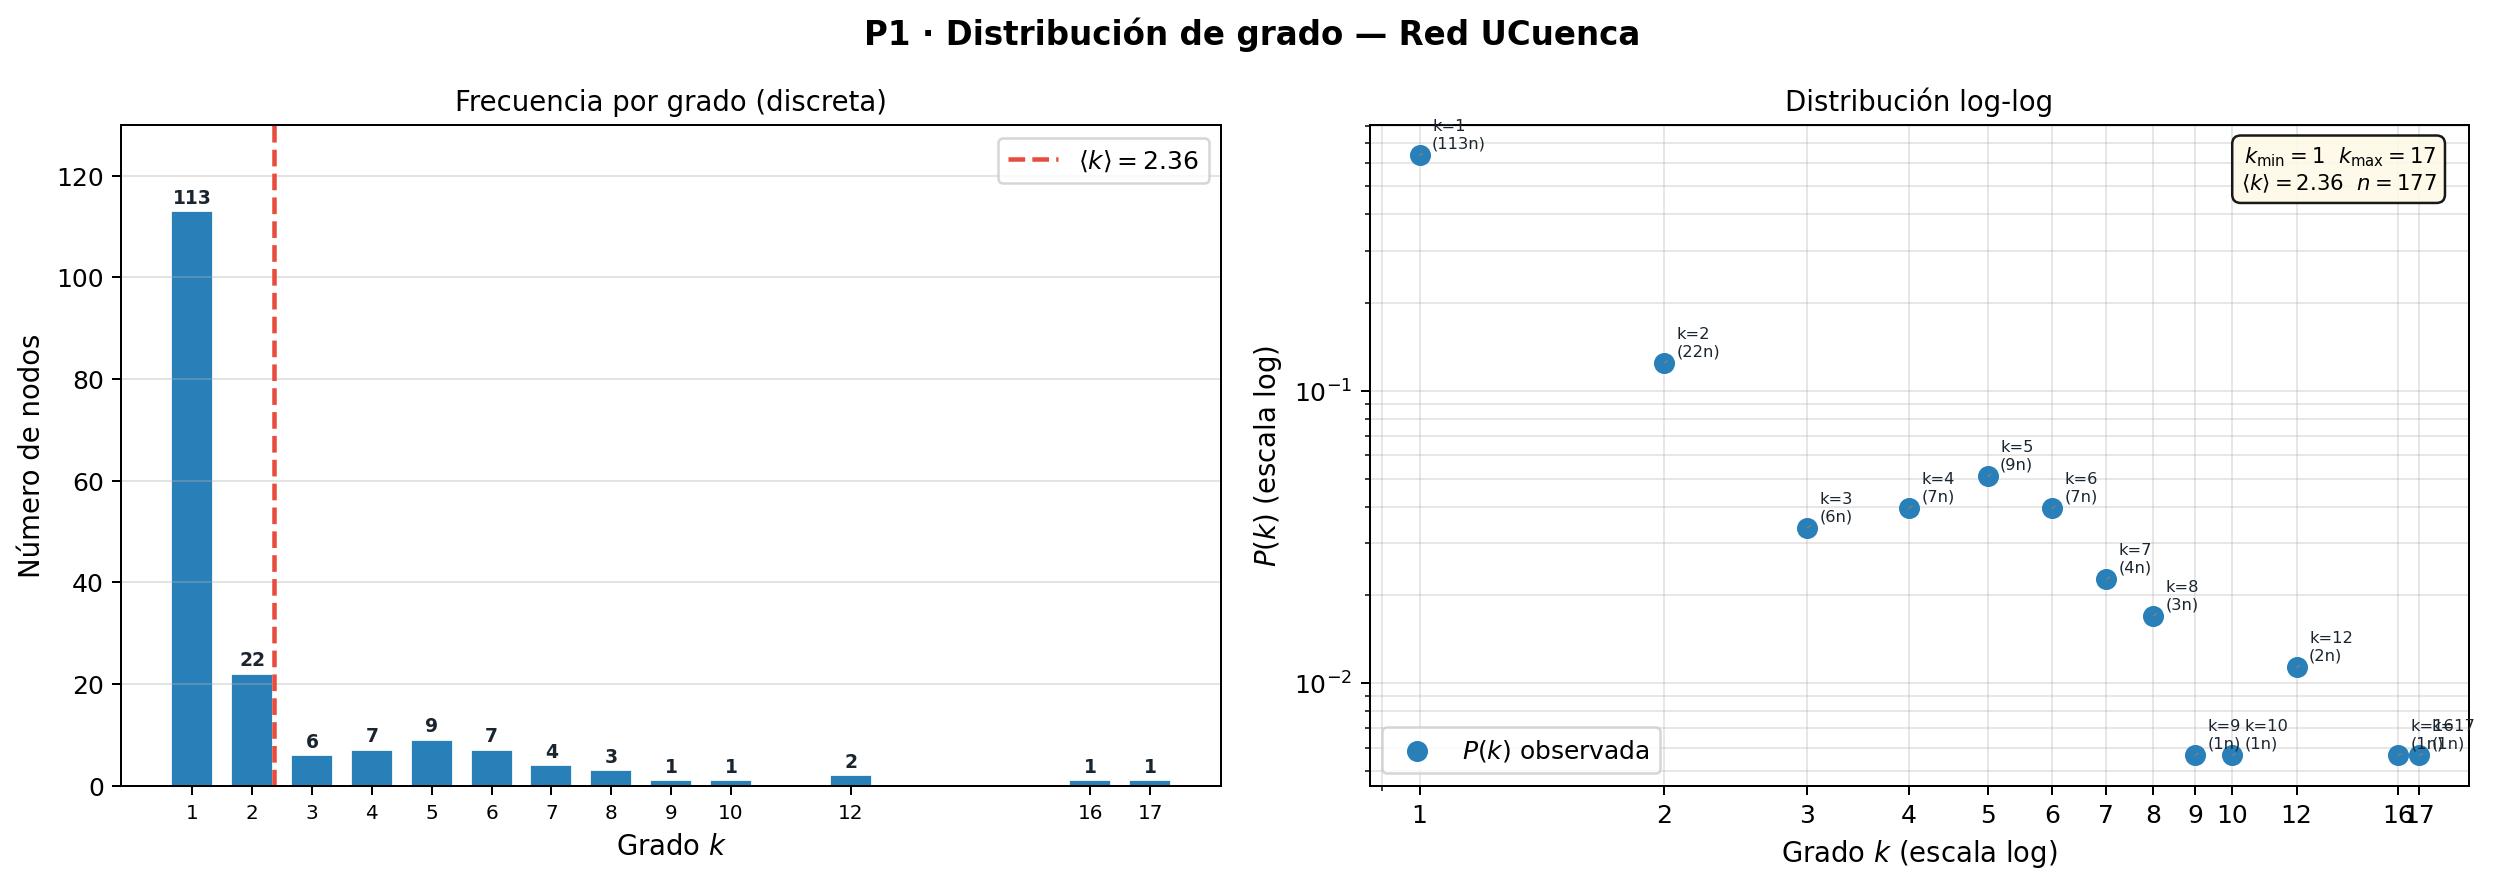
\includegraphics[width=\linewidth]{images/p1_distribucion_grado.png}
        \caption{Distribución de grado $P(k)$ en escala log-log.}
        \label{fig:distribucion_grado}
    \end{subfigure}
    \vspace{0.8cm}  
    \begin{subfigure}[b]{\linewidth}
        \centering
        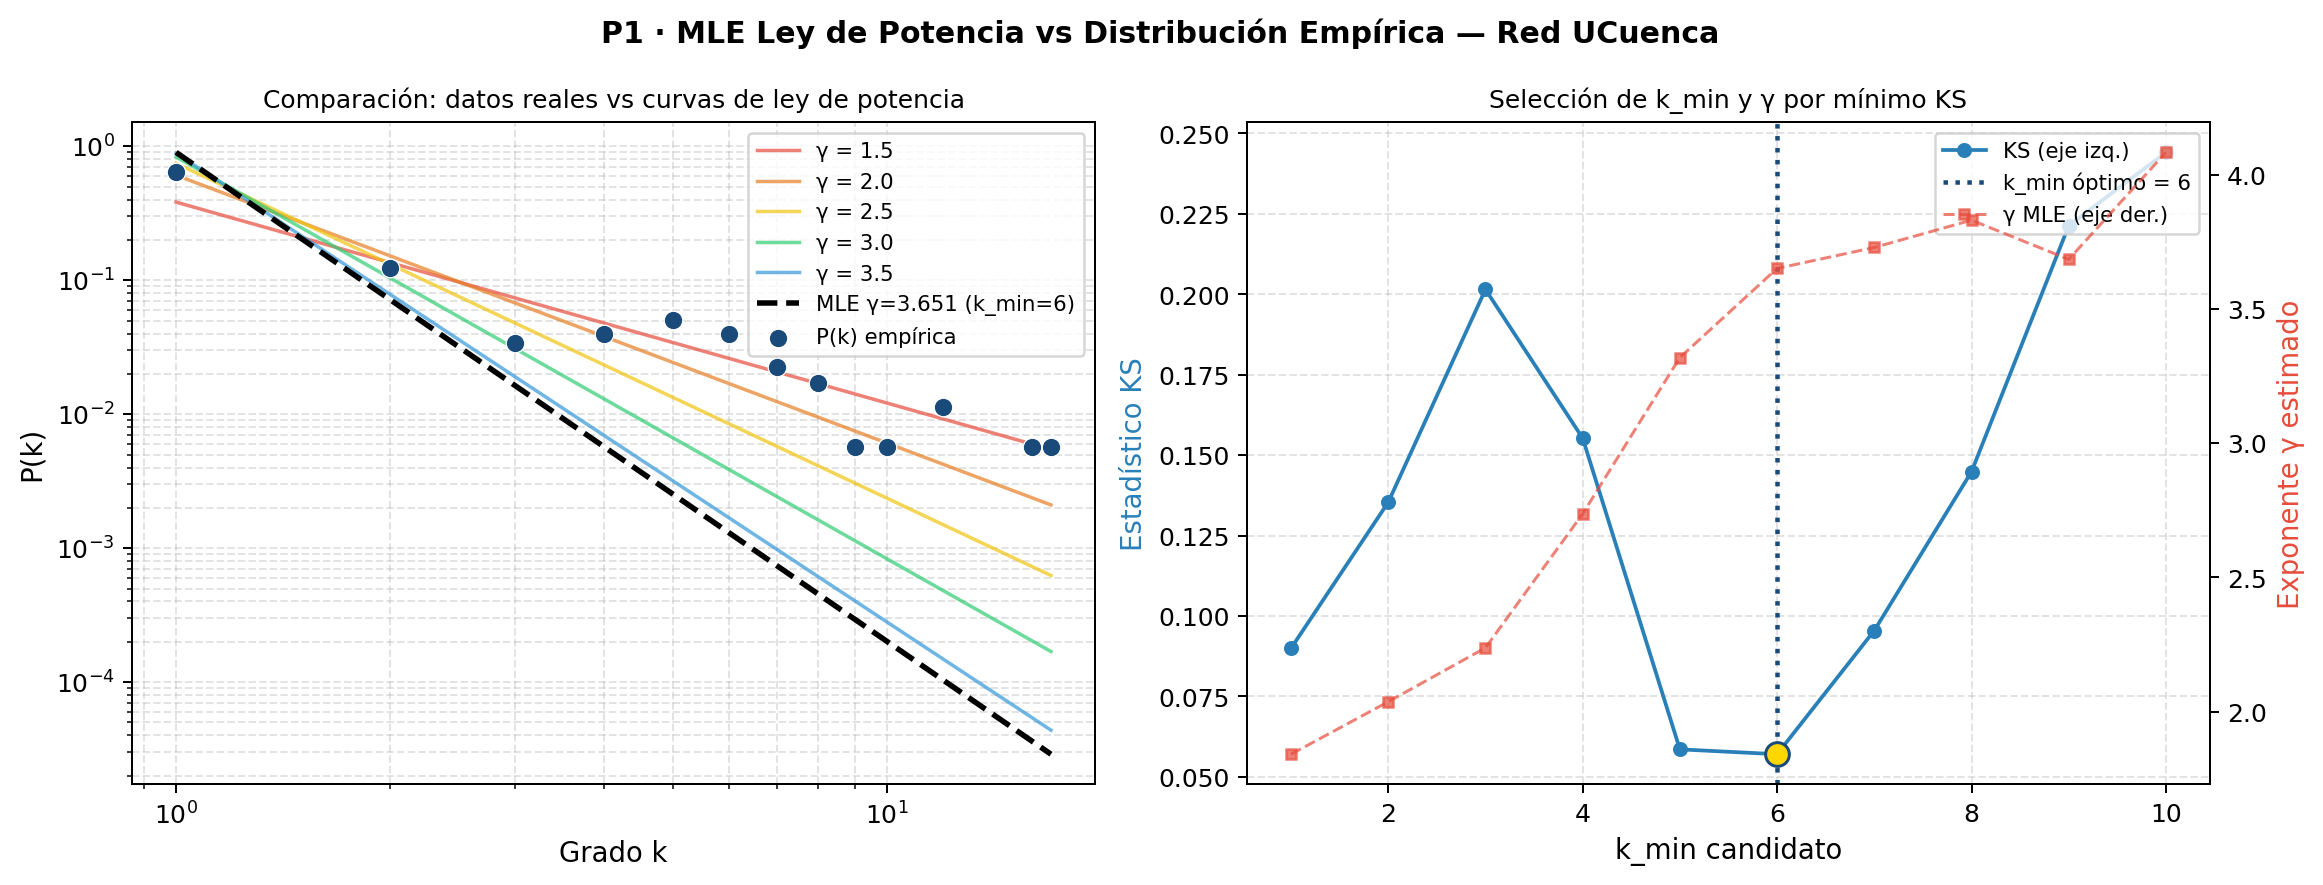
\includegraphics[width=\linewidth]{images/p1_mle_ley_potencia.png}
        \caption{Ajuste MLE: $\alpha = 2.41 \pm 0.18$, $x_{\min}=3$.}
        \label{fig:mle}
    \end{subfigure}
    \caption{Distribución de grado y ajuste de ley de potencia
             (método MLE, Clauset et al., 2009).}
    \label{fig:grado}
\end{figure}

El exponente $\alpha = 2.41$ ($1 < \alpha < 3$) es consistente con una
distribución de ley de potencia. Sin embargo, la cola de la distribución
comprende solo 20 de los 177 nodos ($k \geq x_{\min} = 3$), lo que limita
el poder estadístico del ajuste: el \textit{p}-value del bootstrap de
Clauset et al.\ (2009) es 0.754, lo que no permite rechazar la hipótesis
de ley de potencia pero tampoco la confirma con rigor dado el tamaño reducido
de la cola. En cualquier caso, la heterogeneidad de grado observada produce la
\textit{paradoja de la robustez}: la red es muy resistente a fallos aleatorios
pero frágil ante ataques dirigidos a los hubs.

\subsection{Centralidades y puntos críticos estructurales}

Las cuatro métricas de centralidad utilizadas se definen formalmente:
\begin{align*}
  C_B(v) &= \sum_{s \neq v \neq t} \frac{\sigma_{st}(v)}{\sigma_{st}}
             && \text{(betweenness: fracción de caminos cortos que pasan por } v\text{)} \\[4pt]
  C_C(v) &= \frac{n-1}{\sum_{u \neq v} d(u,v)}
             && \text{(closeness: inverso de la distancia media a todos los nodos)} \\[4pt]
  C_E(v) &= \frac{1}{\lambda_1}\sum_{u \in \mathcal{N}(v)} C_E(u)
             && \text{(eigenvector: proporcional a la centralidad de los vecinos)} \\[4pt]
  C_D(v) &= k_v
             && \text{(grado: número de vecinos directos)}
\end{align*}
Un \textbf{punto de articulación} es un nodo $v$ cuya eliminación aumenta el
número de componentes conexas del grafo. Un \textbf{puente} es una arista
con la misma propiedad. Ambos se detectan en $O(n+m)$ mediante DFS con
tiempos de descubrimiento y de retroceso (algoritmo de Tarjan).

\begin{figure}[H]
    \centering
    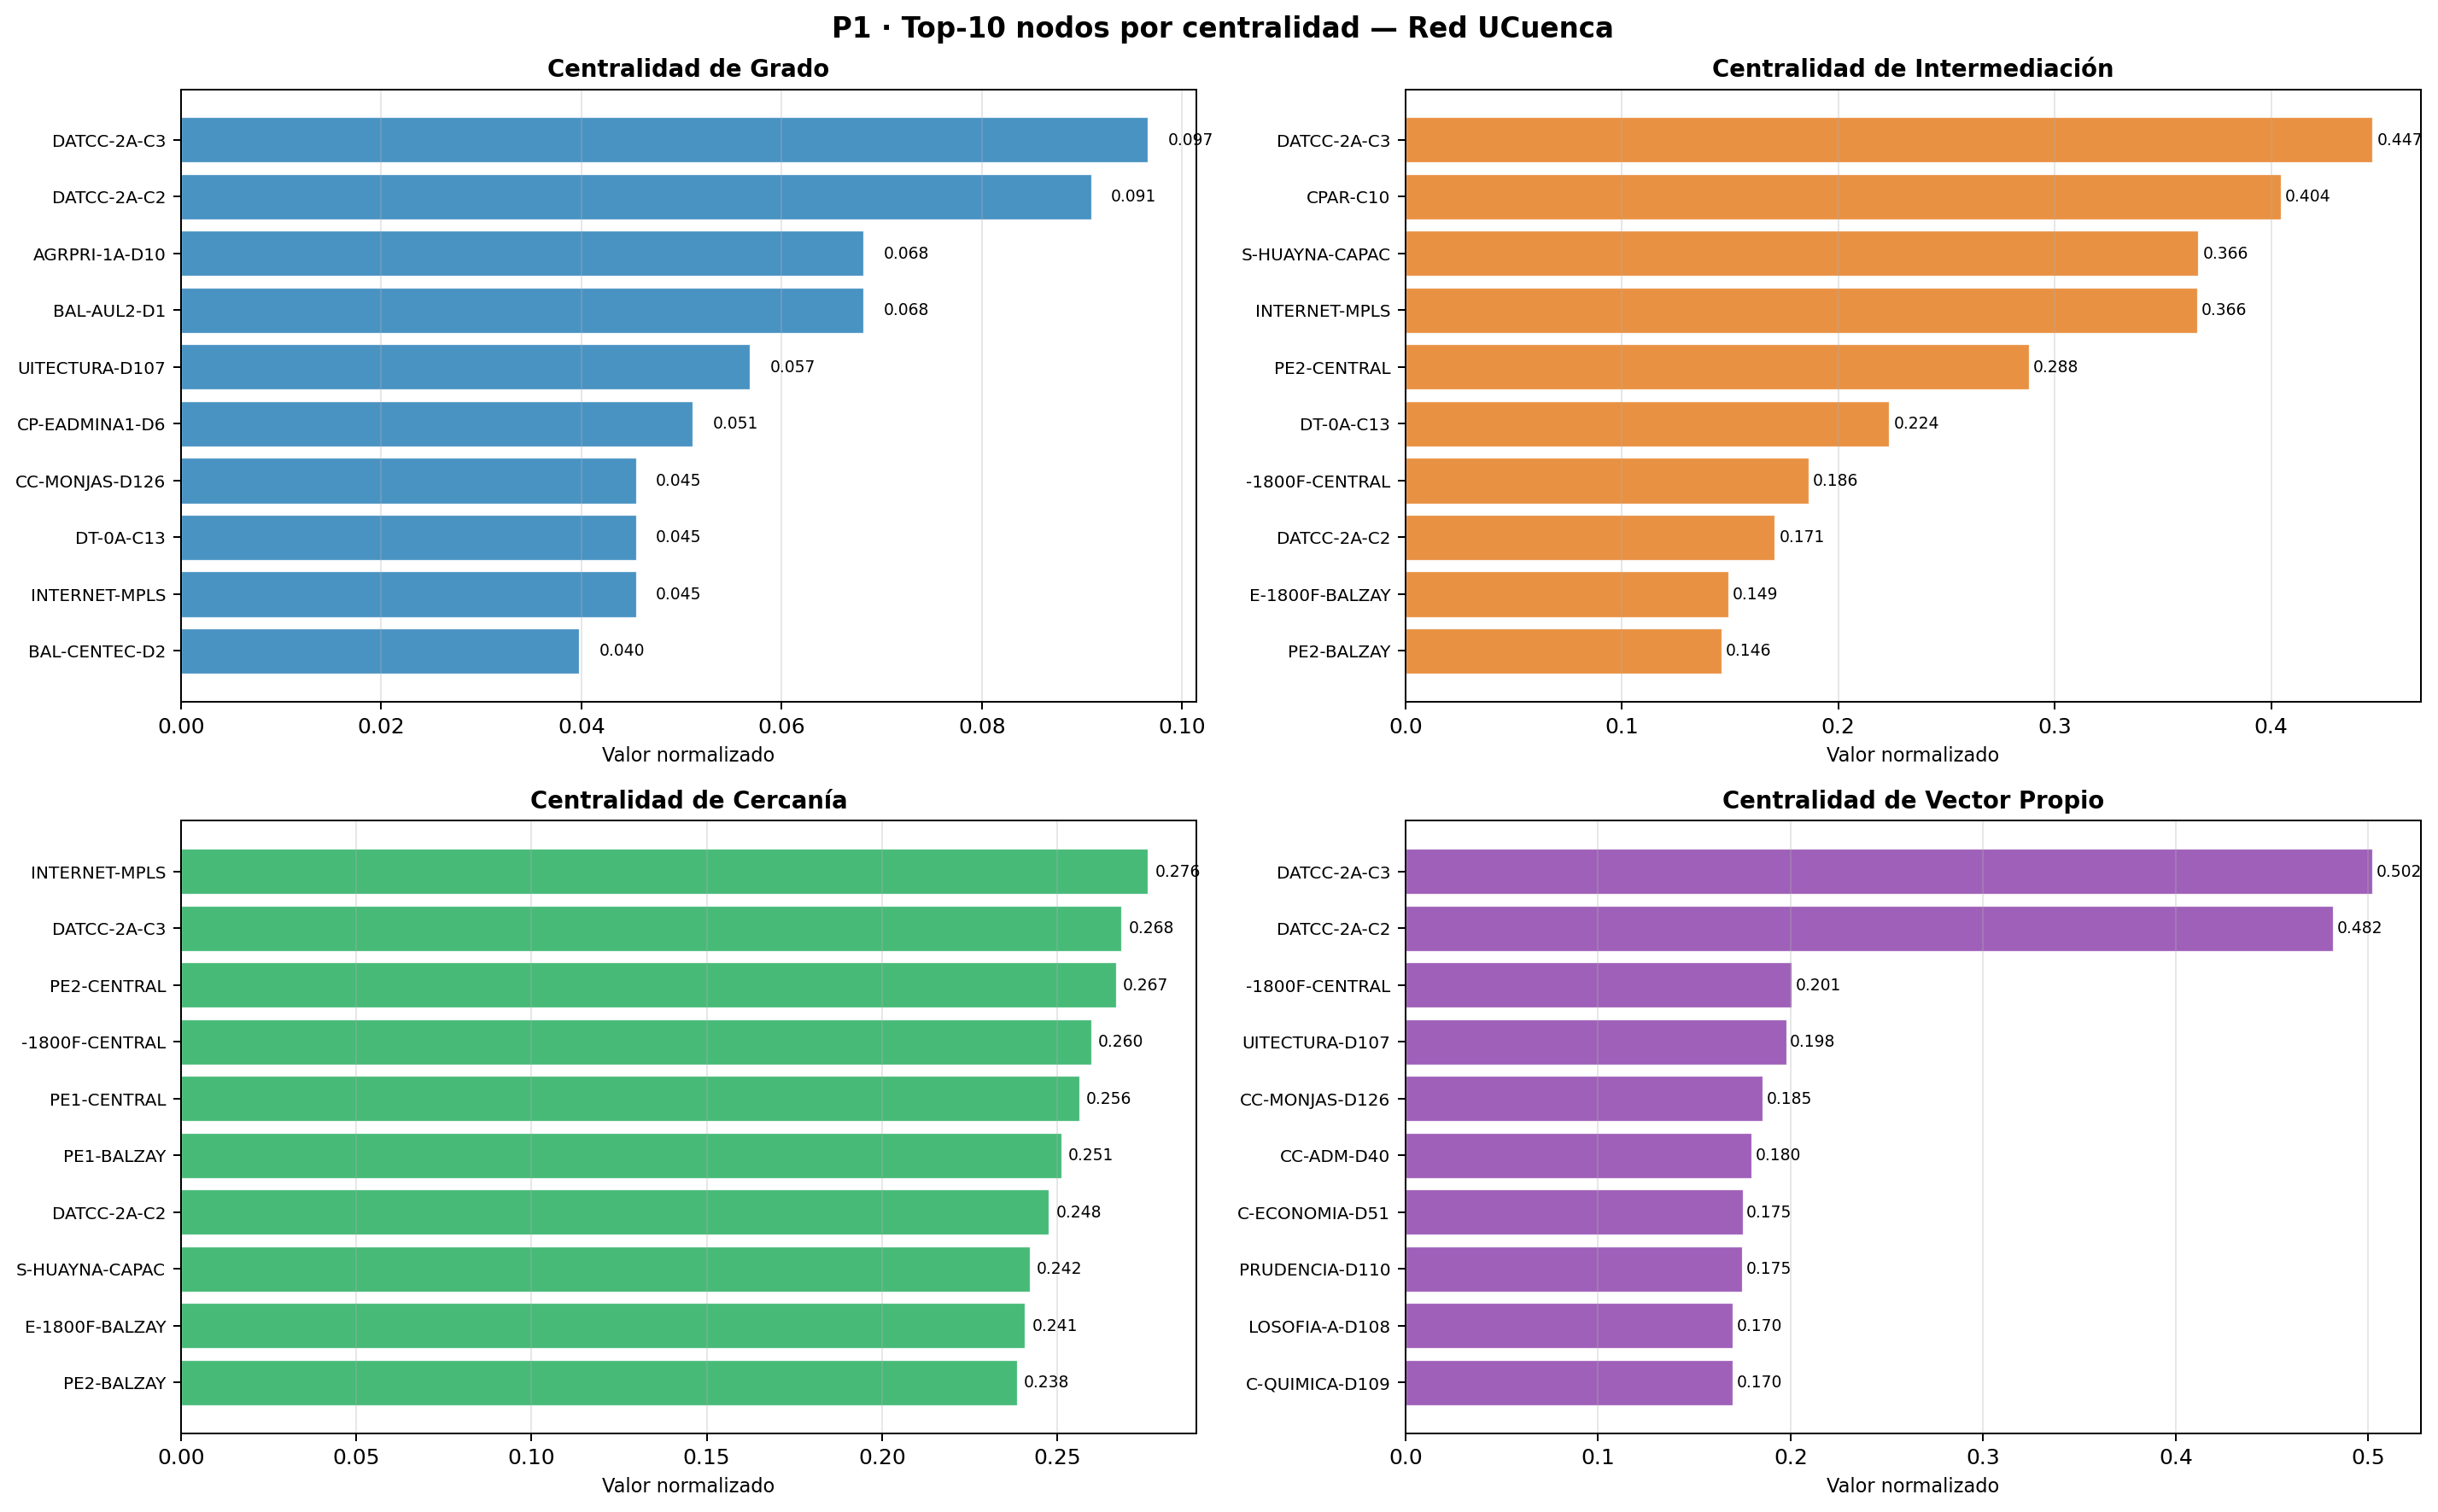
\includegraphics[width=\linewidth]{images/p1_centralidades_top10.png}
    \caption{Top-10 nodos por betweenness, closeness, grado y eigenvector.}
    \label{fig:centralidades}
\end{figure}

\begin{figure}[H]
    \centering
    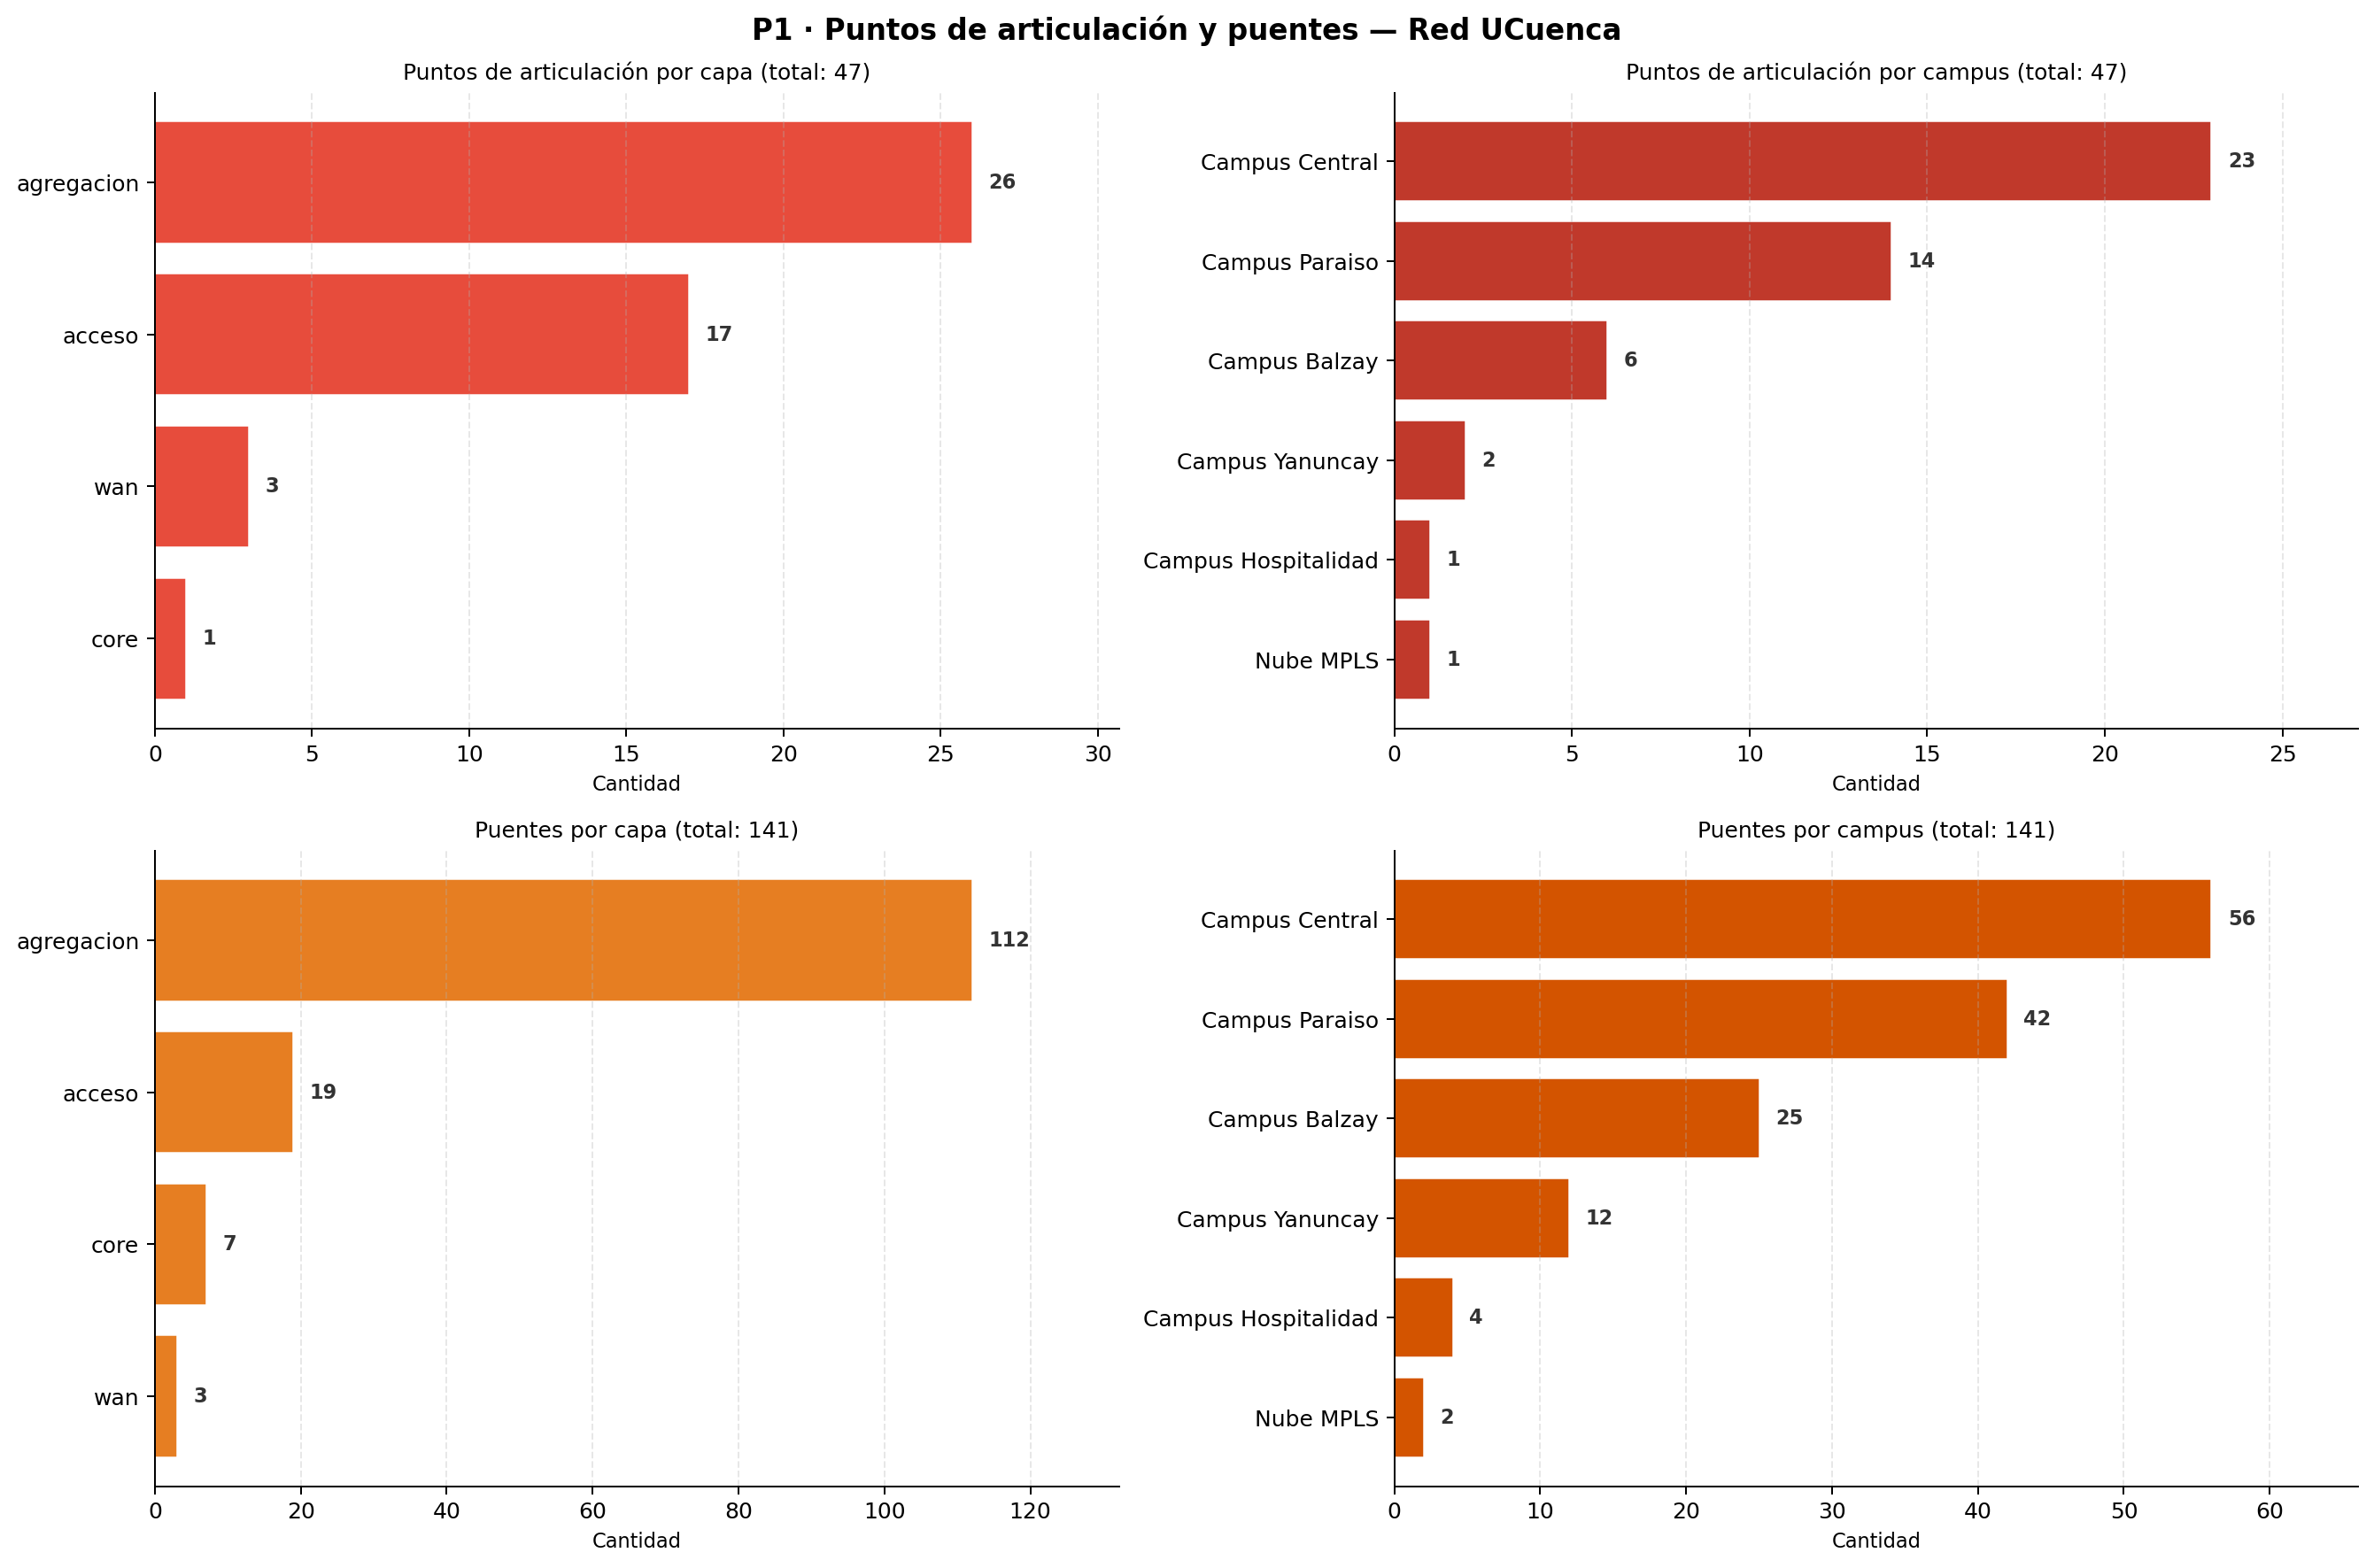
\includegraphics[width=0.9\linewidth]{images/p1_articulacion_puentes.png}
    \caption{Distribución de puntos de articulación y puentes por campus y capa.}
    \label{fig:articulacion}
\end{figure}

La Figura~\ref{fig:betweenness_viz} complementa el análisis mostrando la
red completa con los nodos escalados y coloreados según su betweenness,
lo que permite identificar visualmente los equipos que concentran el mayor
flujo de caminos cortos.

\begin{figure}[H]
    \centering
    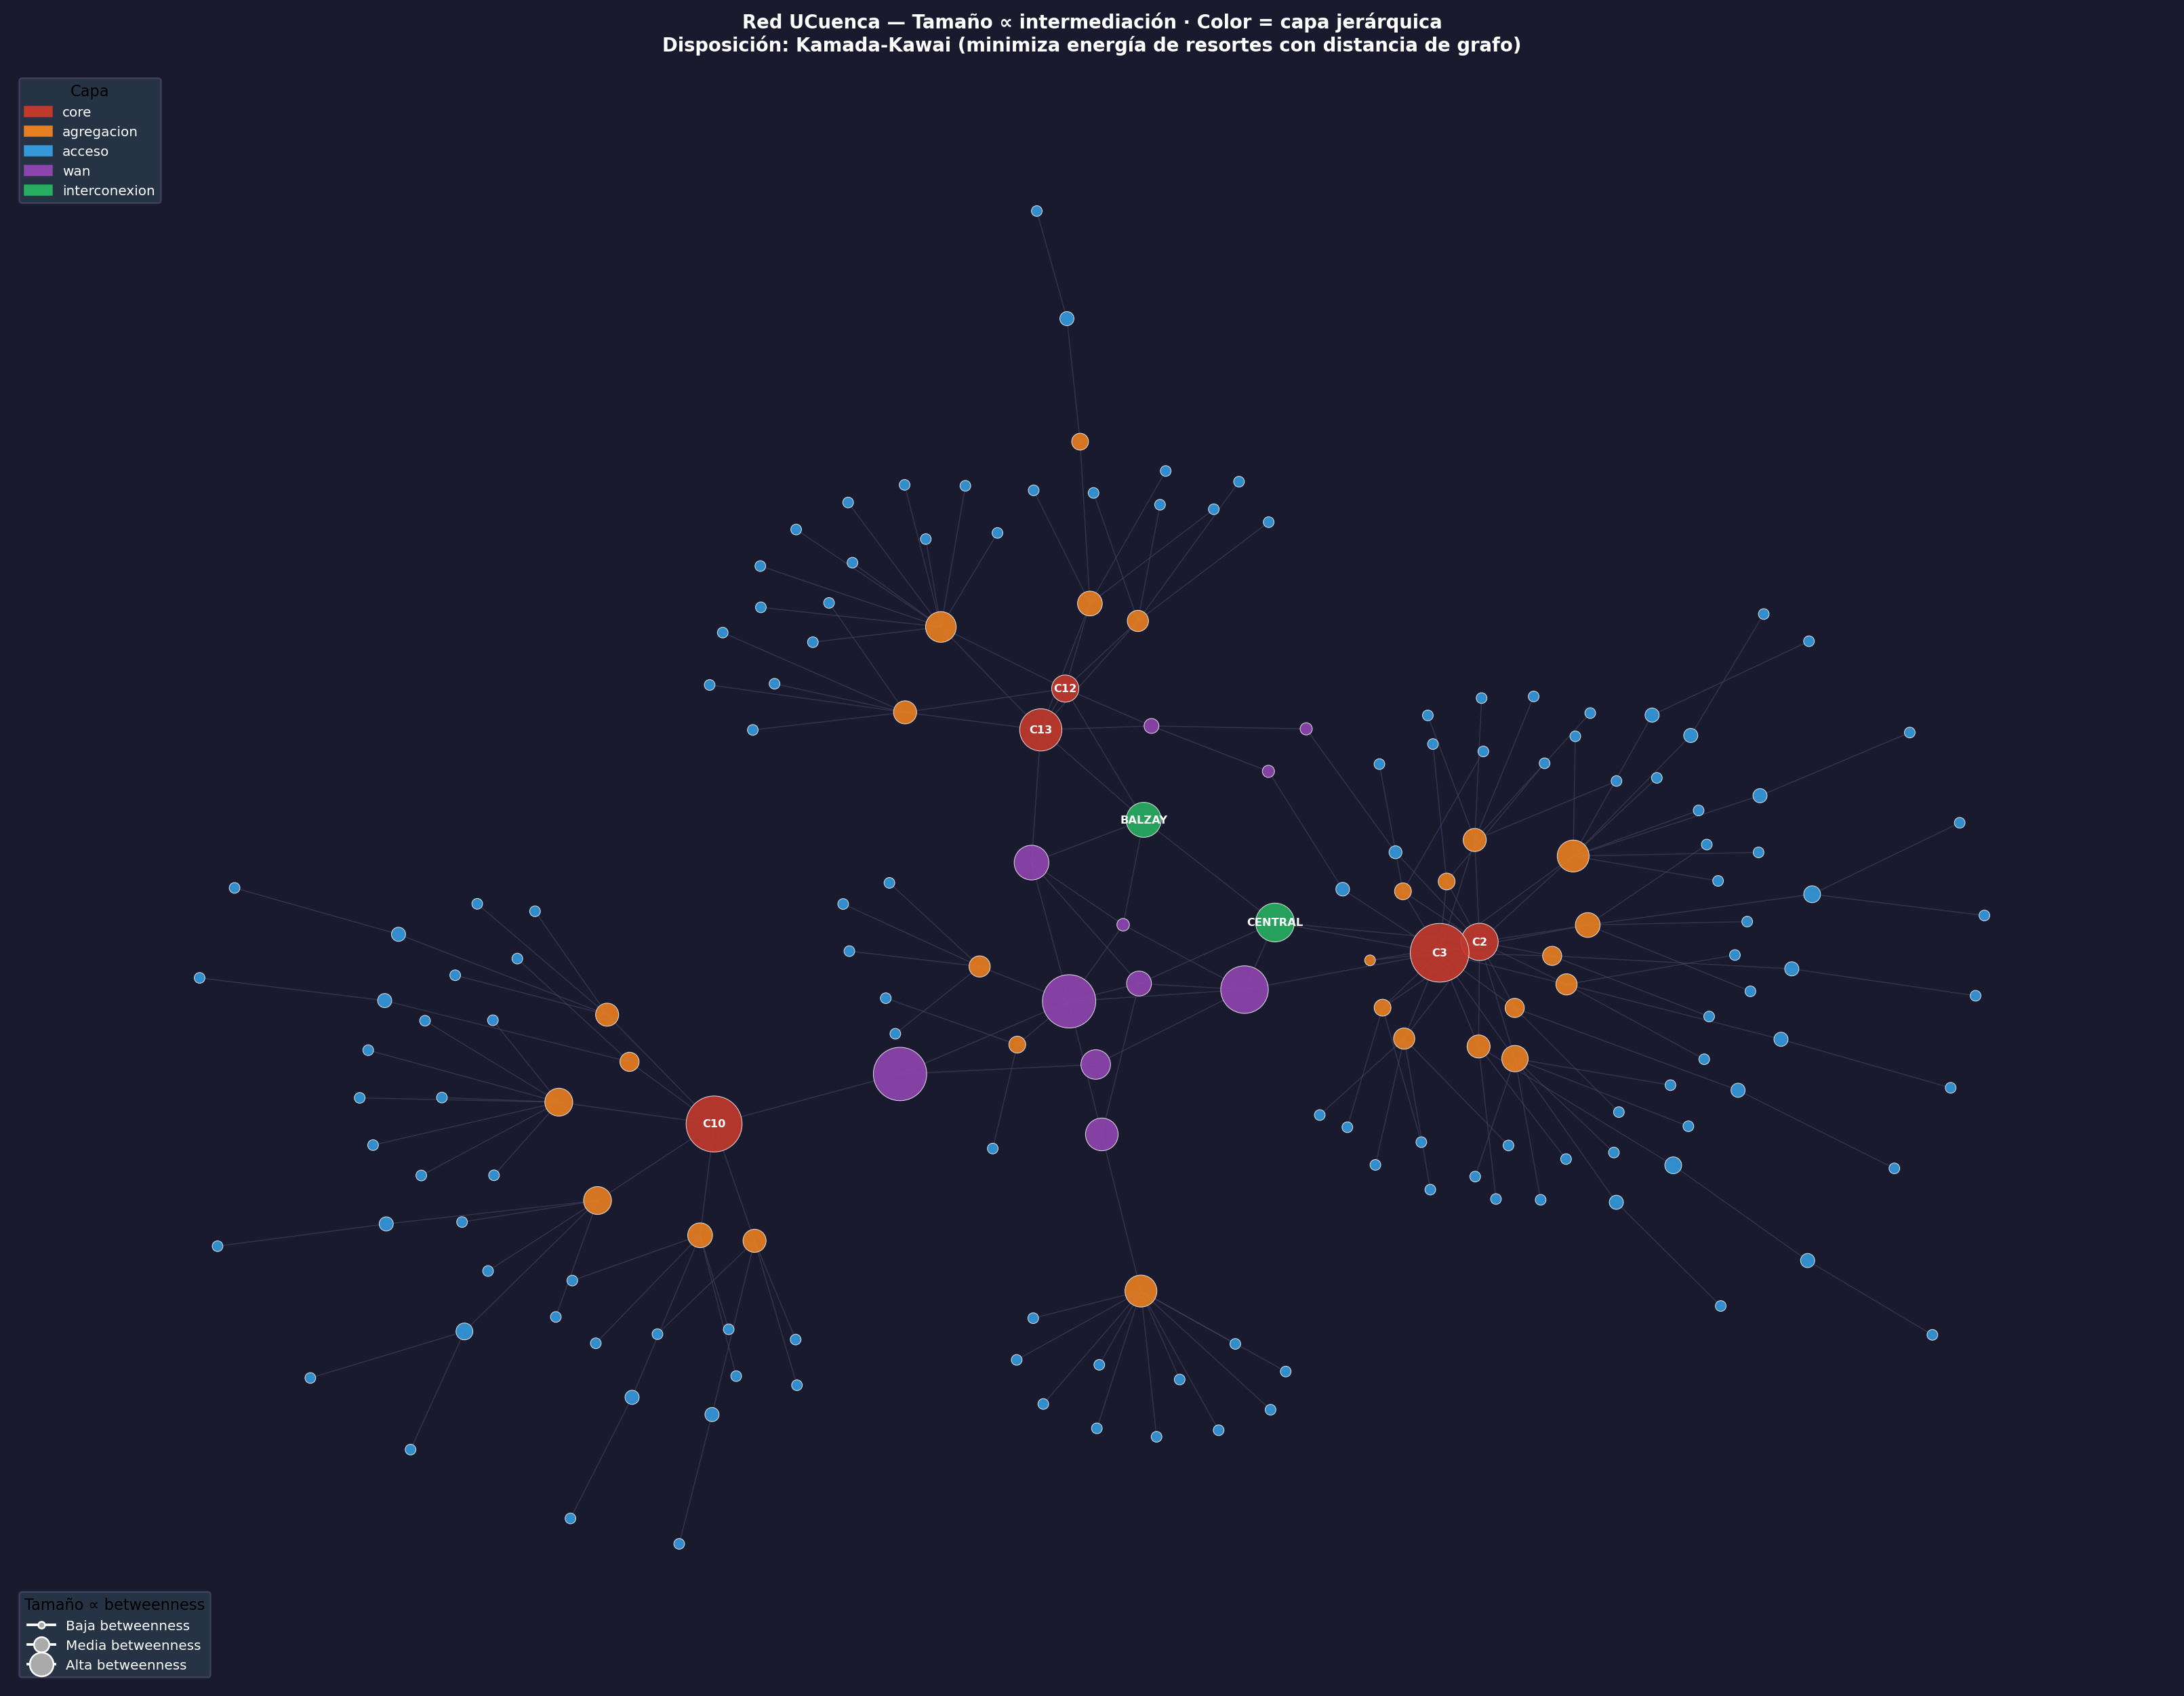
\includegraphics[width=0.7\linewidth]{images/p2_visualizacion_betweenness.png}
    \caption{Red UCuenca con nodos escalados y coloreados por betweenness.
             Los nodos de mayor tamaño y color más intenso son los principales
             intermediarios de la red.}
    \label{fig:betweenness_viz}
\end{figure}

La Figura~\ref{fig:centralidades} presenta el ranking de los 10 nodos más
centrales según betweenness, closeness, grado y eigenvector.
\texttt{DATCC-2A-C3} (core, Campus Central) encabeza las cuatro métricas:
grado 17, betweenness 0.447, closeness 0.268 y eigenvector 0.502.
La Figura~\ref{fig:articulacion} desglosa los puntos de articulación y puentes
por campus y por capa (core, agregación, acceso): el Campus Central concentra
23 de los 47 puntos de articulación, lo que refleja su rol de concentrador
institucional.

\subsection{Modelos nulos y comparación estructural}

Se comparan tres modelos nulos con la red real:
\begin{itemize}
  \item \textbf{Erdős-Rényi (ER):} cada par de nodos se conecta con
        probabilidad $p = 2m/[n(n-1)]$; grados siguen una Poisson.
  \item \textbf{Modelo de Configuración (CM):} preserva la secuencia de
        grados real $\{k_v\}$ pero asigna enlaces al azar (reconexión de
        \textit{stubs}). Referencia directa: mismos grados, sin estructura.
  \item \textbf{Barabási-Albert (BA):} crece con adjunción preferencial
        $\Pi(k) \propto k$; produce $P(k) \sim k^{-3}$ y es el modelo
        canónico de redes libre de escala.
\end{itemize}

\begin{figure}[H]
    \centering
    \begin{subfigure}[b]{0.8\linewidth}
        \centering
        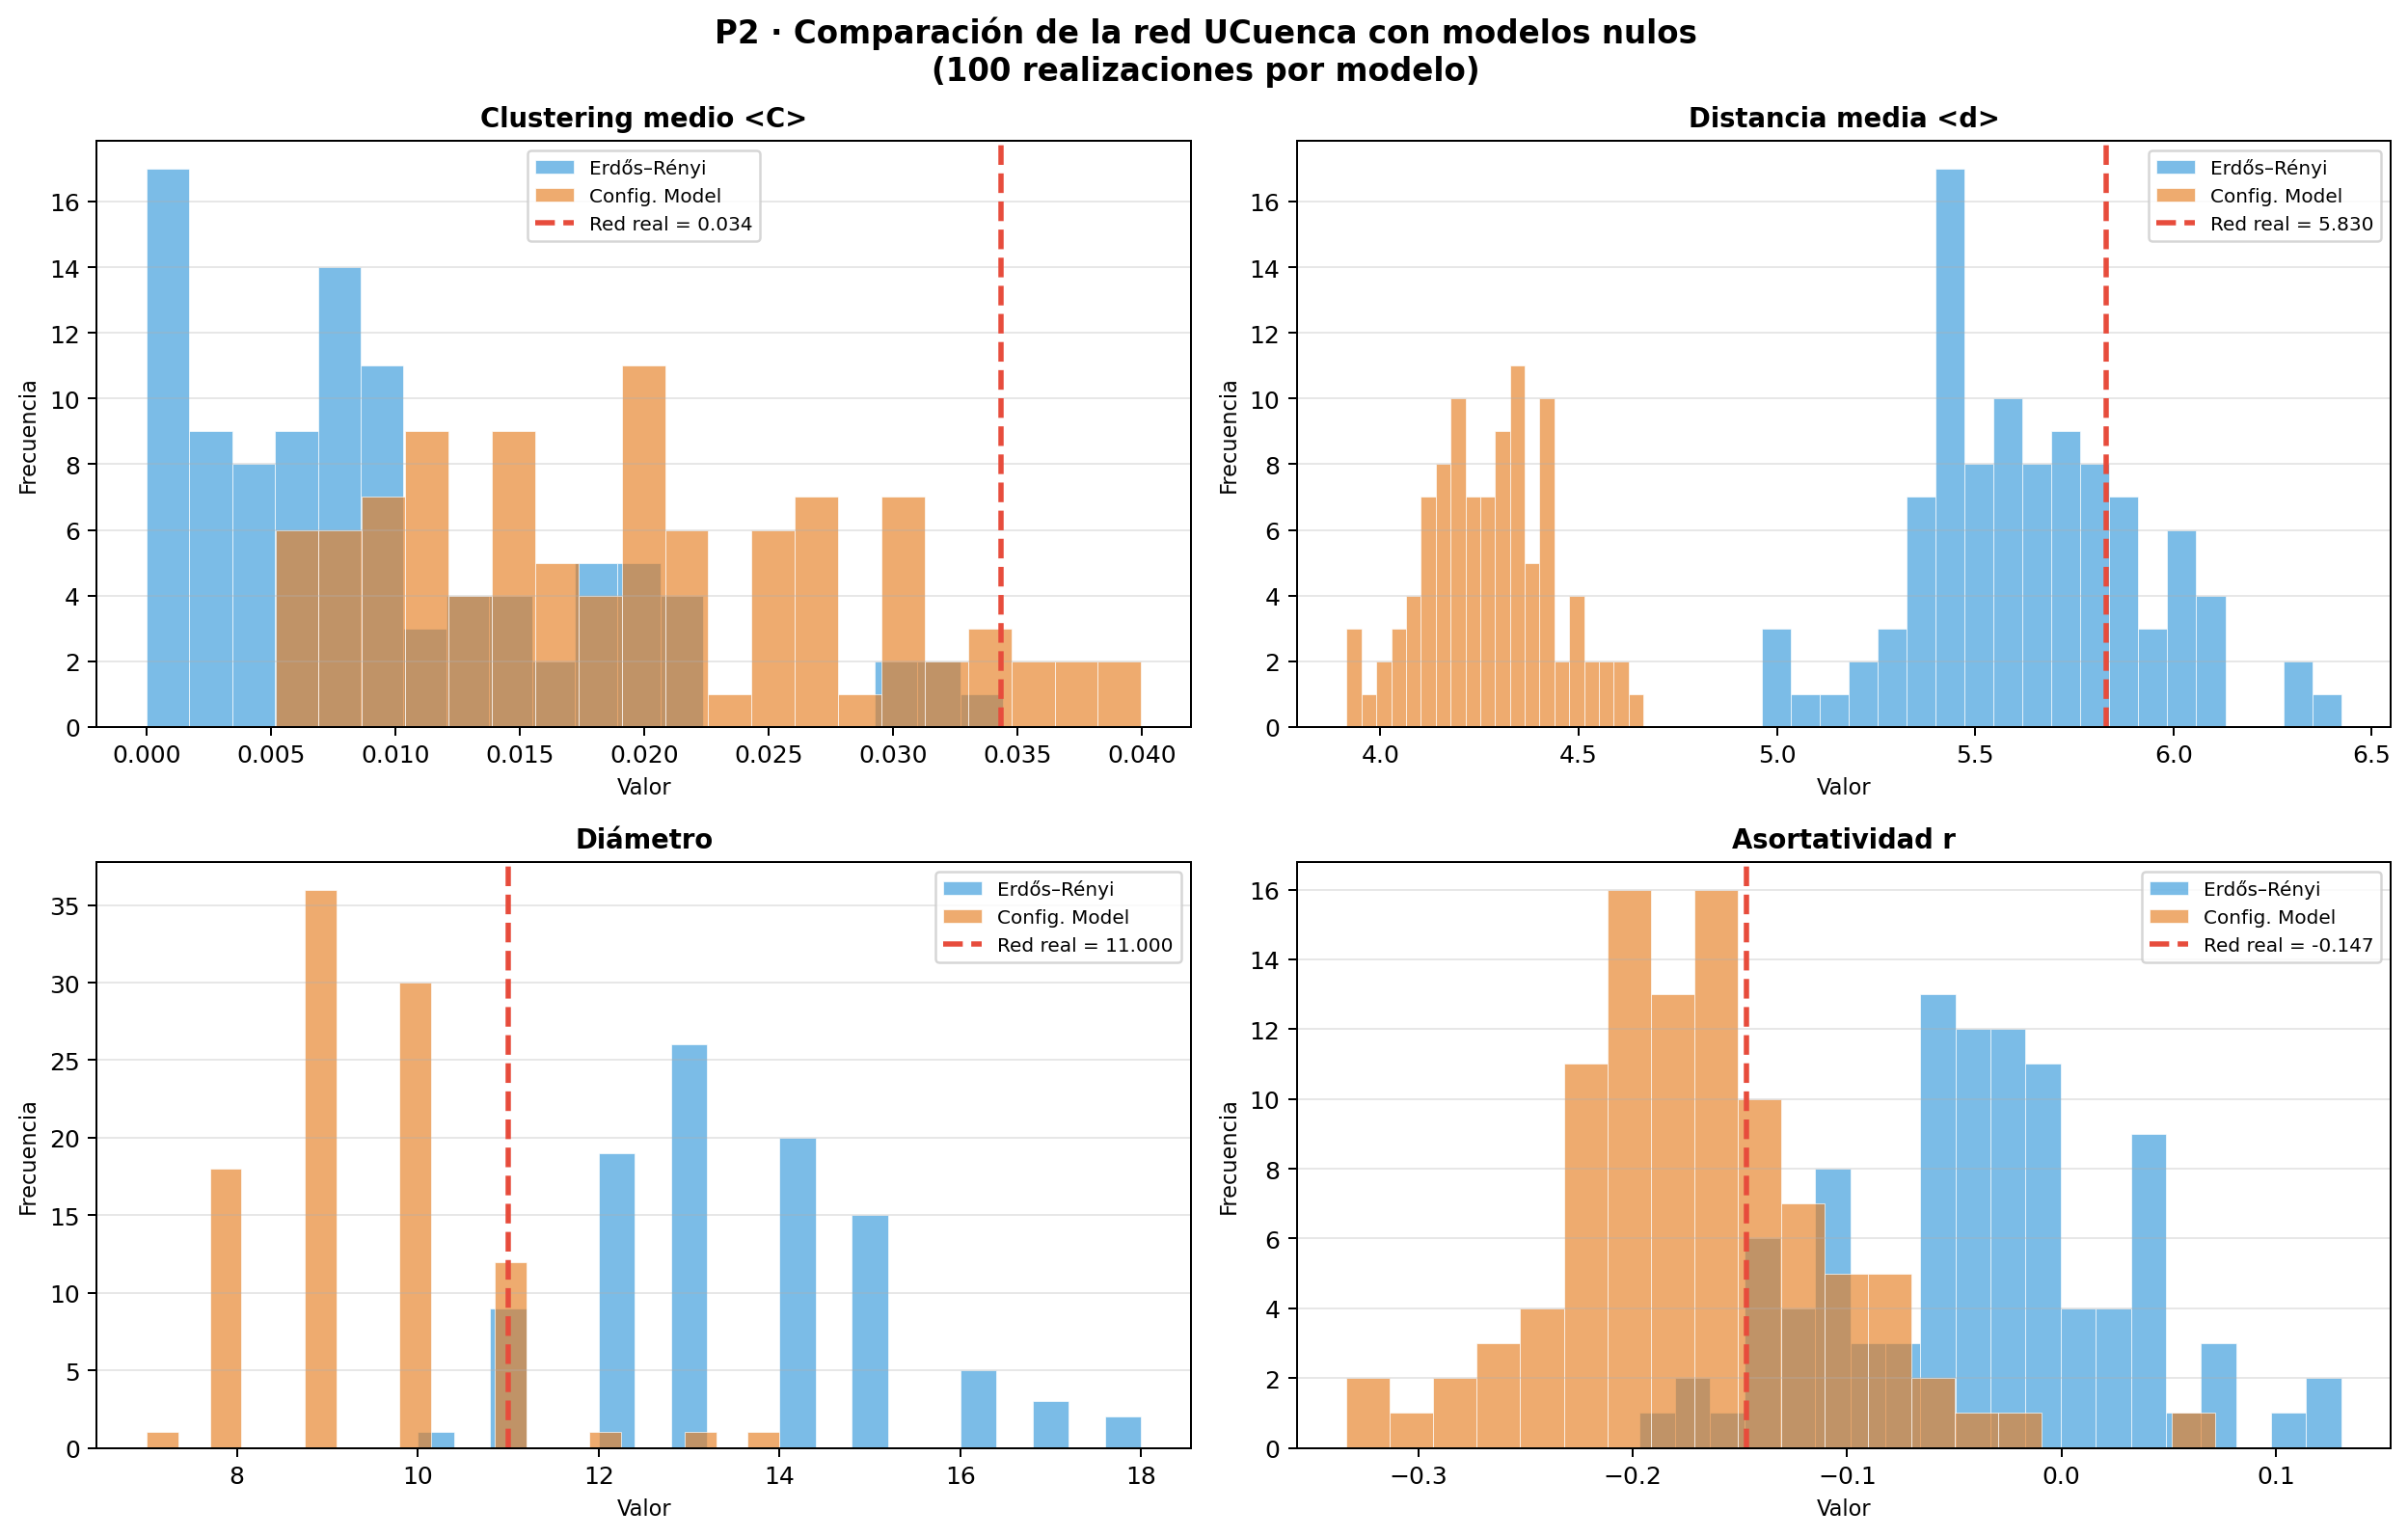
\includegraphics[width=\linewidth]{images/p2_comparacion_modelos.png}
        \caption{Comparación de métricas: UCuenca vs.\ ER, CM y BA.}
        \label{fig:comparacion_modelos}
    \end{subfigure}
    \vspace{0.5cm}
    \begin{subfigure}[b]{0.8\linewidth}
        \centering
        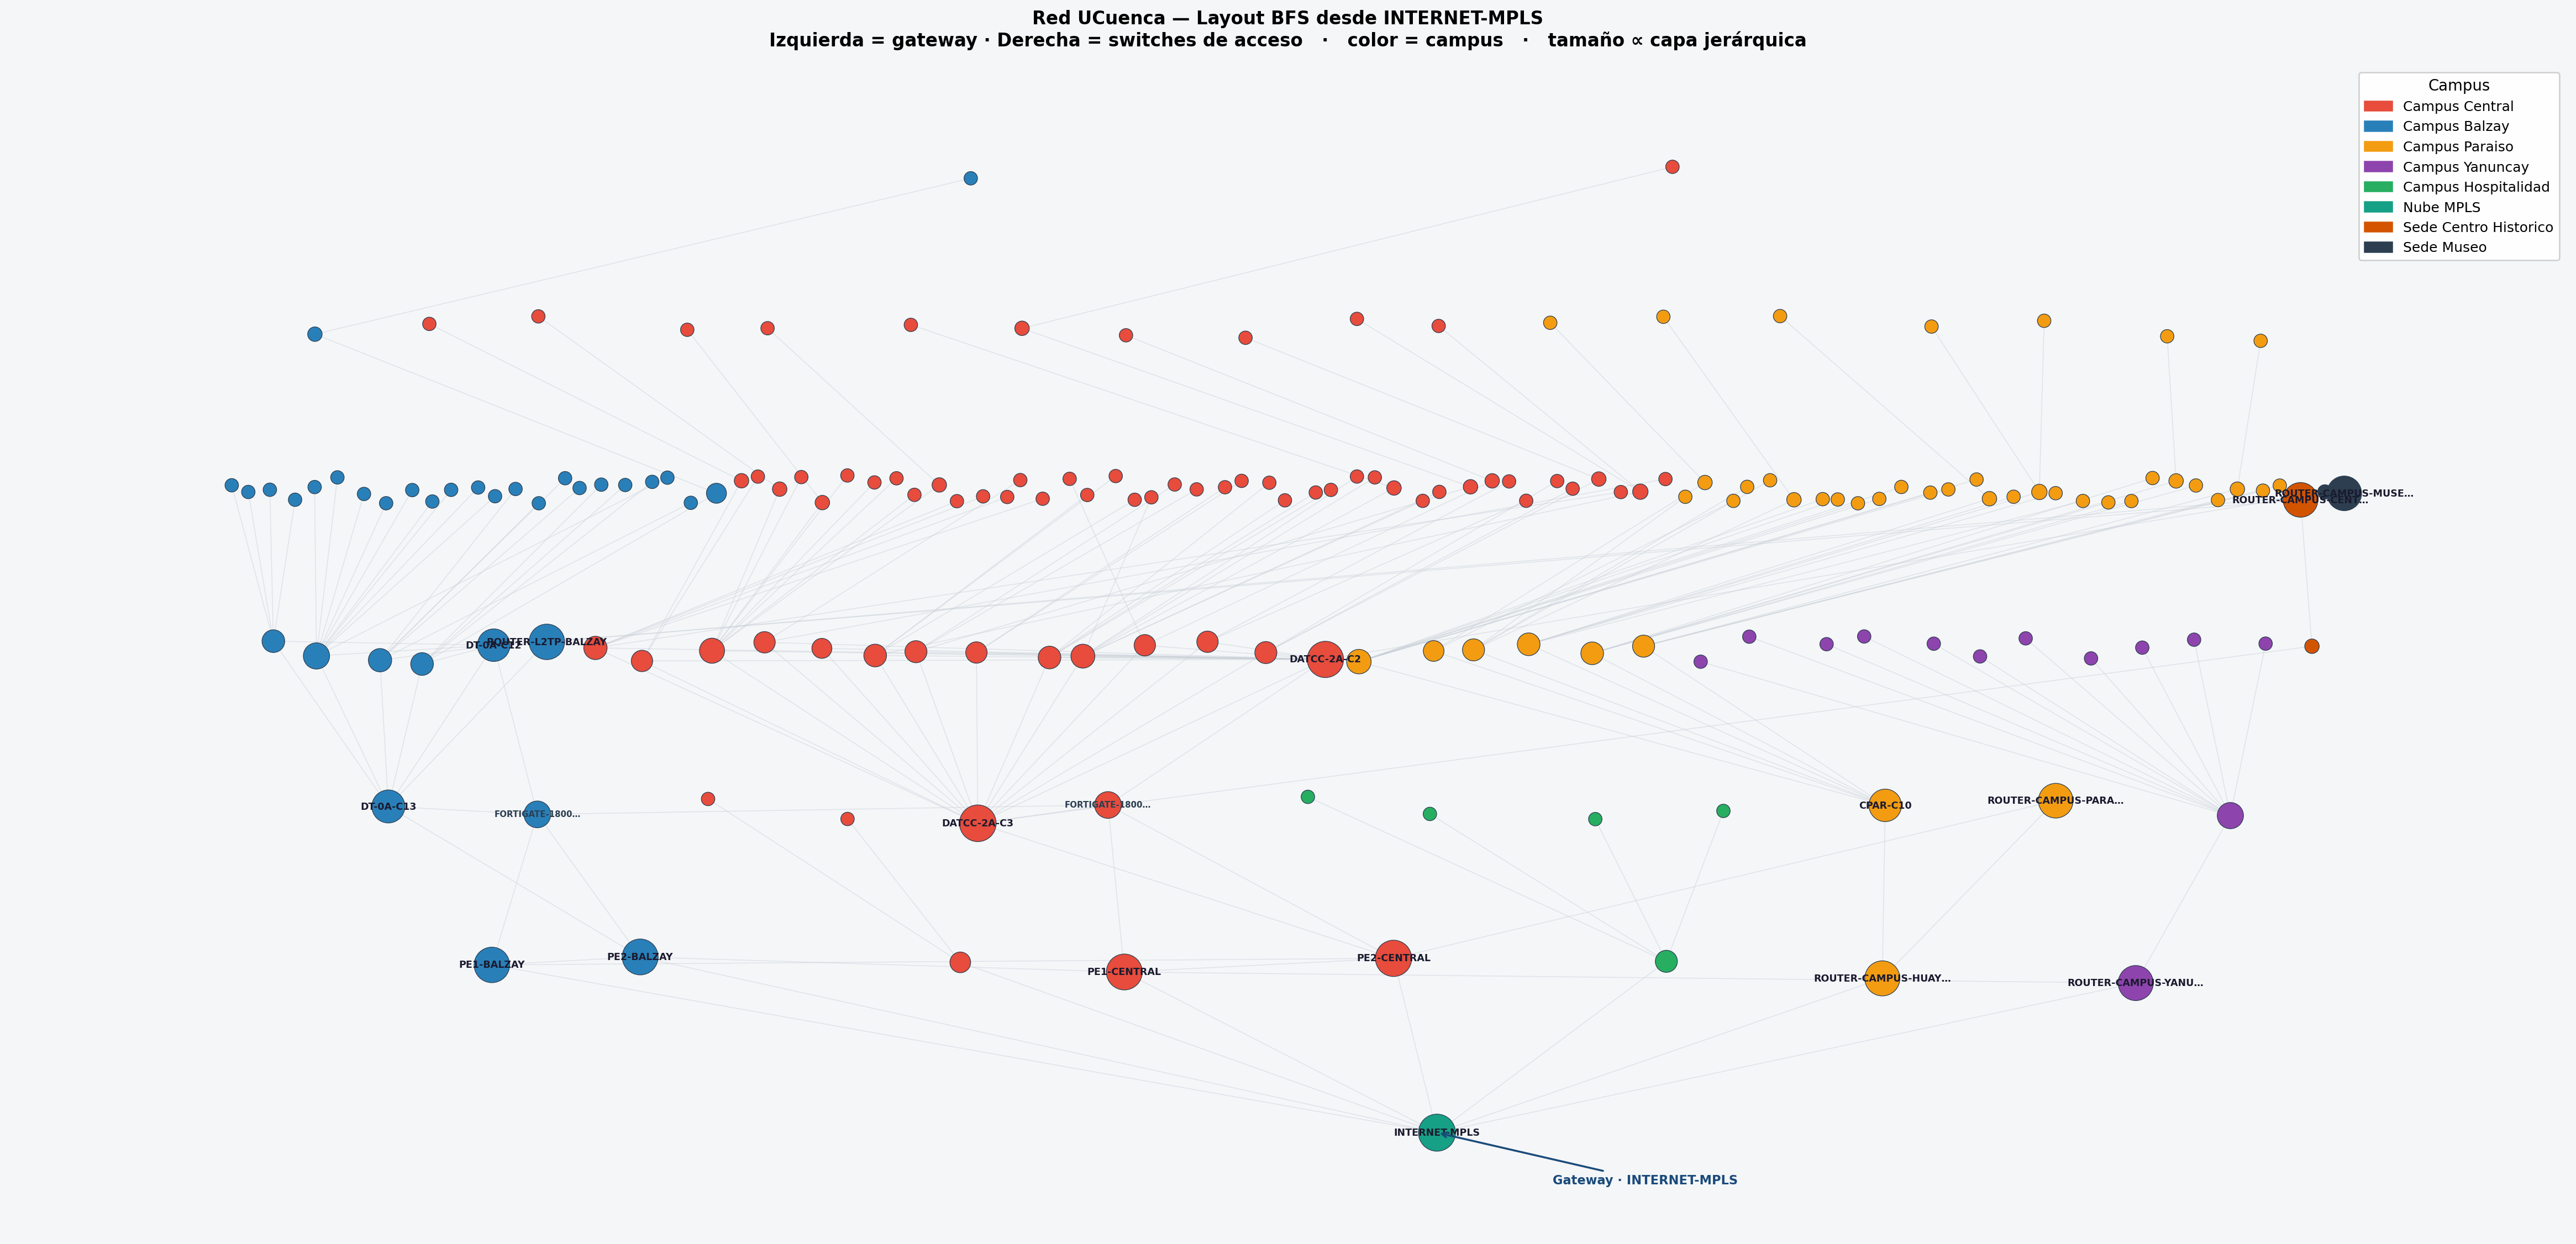
\includegraphics[width=\linewidth]{images/p2_visualizacion_campus.png}
        \caption{Visualización de la red coloreada por campus.}
        \label{fig:visualizacion}
    \end{subfigure}
    \caption{Contraste con modelos nulos y visualización topológica.}
    \label{fig:modelos}
\end{figure}

La Figura~\ref{fig:barabasi} muestra un grafo Barabási-Albert generado
con los mismos parámetros que UCuenca ($n=177$, $m \approx 209$),
ilustrando la topología \textit{hub-and-spoke} característica del modelo
de adjunción preferencial: pocos nodos de grado muy alto conectados a
muchos nodos de grado bajo.

\begin{figure}[H]
    \centering
    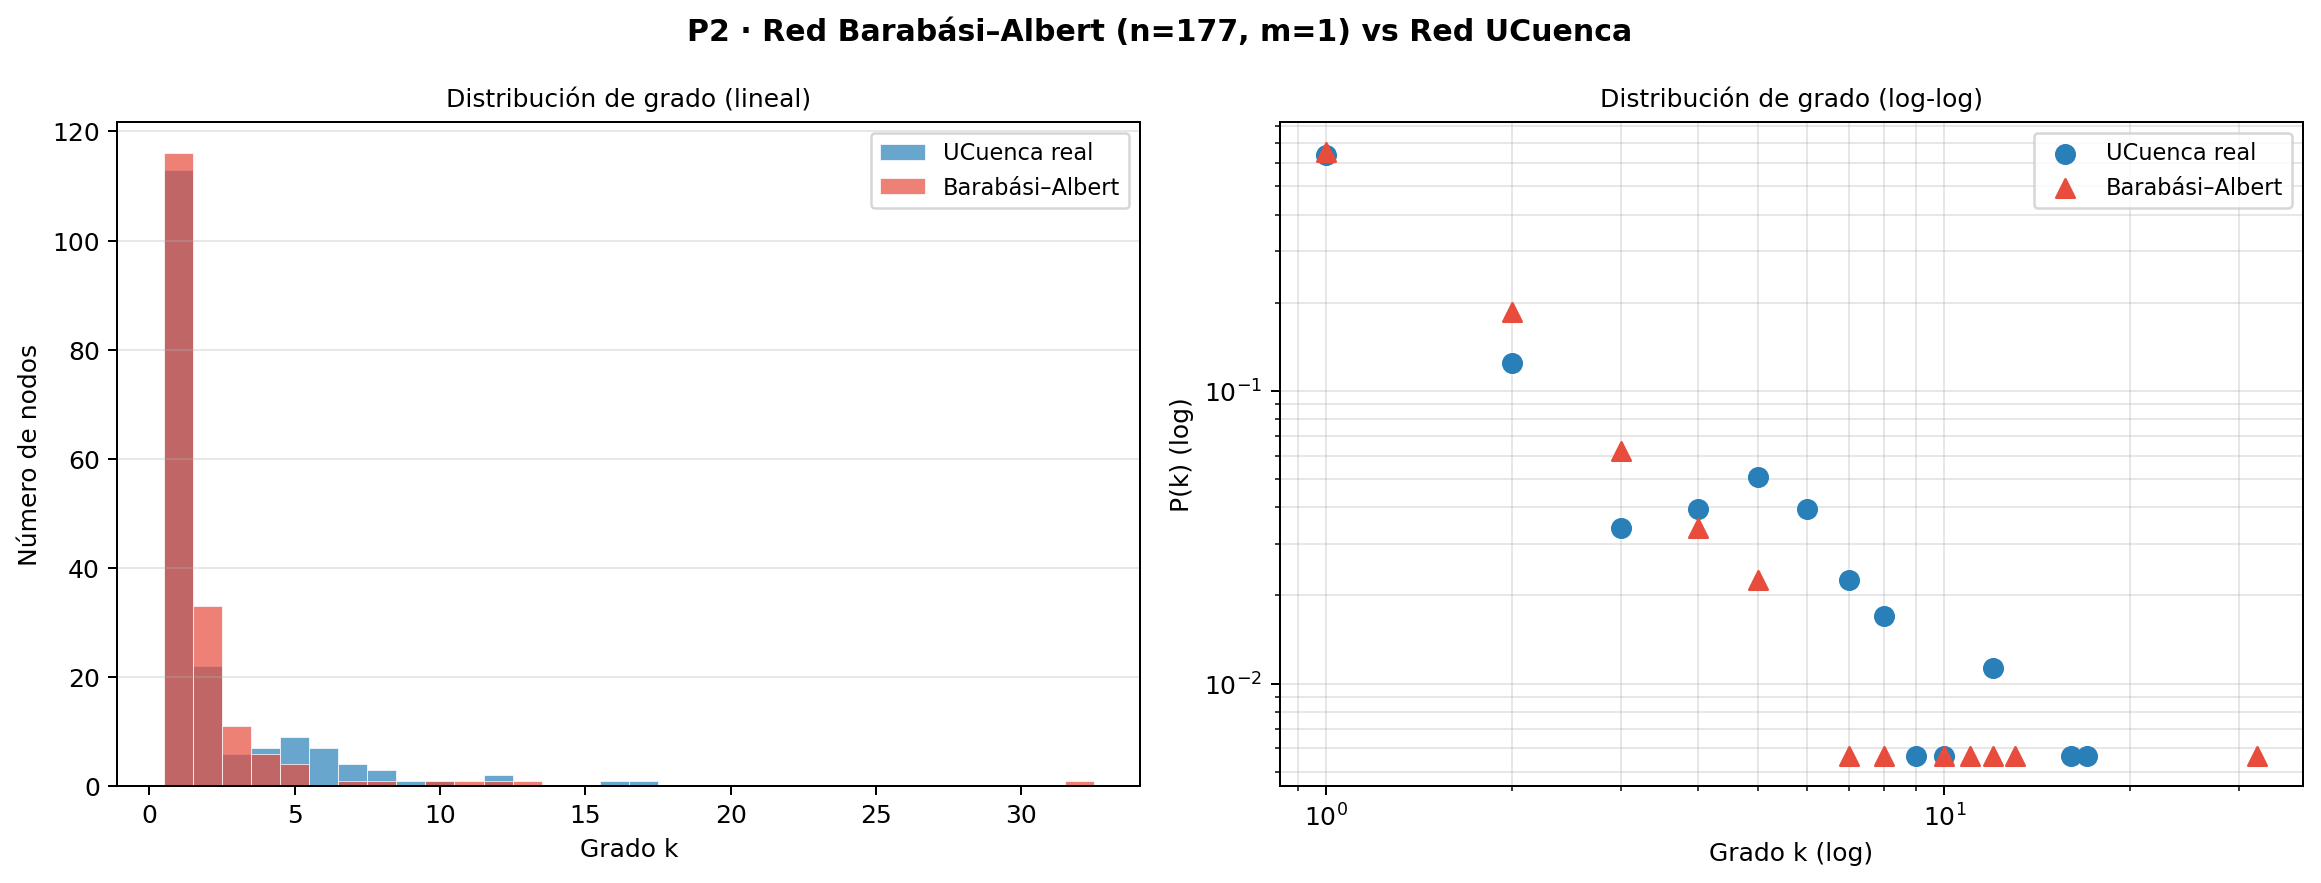
\includegraphics[width=0.75\linewidth]{images/p2_barabasi_albert.png}
    \caption{Grafo Barabási-Albert sintético ($n=177$) para comparación
             visual con la topología real de UCuenca.}
    \label{fig:barabasi}
\end{figure}

La Figura~\ref{fig:modelos}a compara visualmente las métricas de UCuenca
(distancia media, clustering, eficiencia global y asortatividad) frente a
los tres modelos nulos; la Figura~\ref{fig:modelos}b muestra la topología
real coloreada por campus, donde se aprecia la estructura jerárquica
core–agregación–acceso y el aislamiento geográfico entre sedes.
La Tabla~\ref{tab:modelos_nulos} resume la comparación con tres modelos nulos.

\begin{table}[H]
\centering
\caption{Comparación de la red UCuenca con modelos nulos ($n=177$, $m=209$).}
\label{tab:modelos_nulos}
\small
\begin{tabular}{L{3.5cm} C{2.2cm} C{2.2cm} C{2.2cm} C{2.2cm}}
    \toprule
    \encabezado{Métrica} &
    \encabezado{UCuenca} &
    \encabezado{ER} &
    \encabezado{Conf. Model} &
    \encabezado{BA} \\
    \midrule
    \rowcolor{tabfila}
    Distancia media     & 5.83  & 5.21  & 5.95  & 4.86 \\
    Clust. global       & 0.019 & 0.013 & 0.014 & 0.032 \\
    \rowcolor{tabfila}
    $P(k)$ forma        & Ley potencia & Poisson & Real & Pot. ($\gamma=3$) \\
    Asortatividad       & $-$0.15 & $\approx 0$ & $-$0.17 & $-$0.09 \\
    \rowcolor{tabfila}
    Eficiencia global   & 0.208 & 0.233 & 0.192 & 0.265 \\
    \bottomrule
\end{tabular}
\end{table}

La red UCuenca es \textbf{menos eficiente} que el modelo ER (0.208 vs.\
0.233) aunque preserva la secuencia de grados real. Esto evidencia que la
topología específica ---las conexiones concretas entre nodos--- es
\textit{subóptima} respecto a una configuración aleatoria con los mismos
grados. La asortatividad negativa ($-0.15$) indica que los hubs tienden a
conectarse con nodos de bajo grado (estructura estrella/árbol), típica de
redes de infraestructura diseñadas.

% ============================================================
%  5. RECORRIDOS Y COMUNIDADES — FASE 2
% ============================================================
\section{Recorridos y comunidades (Fase~2)}

\subsection{Análisis de k-core y estructura de ciclos}

El \textbf{$k$-core} de un grafo es el subgrafo maximal en que todo nodo
tiene grado $\geq k$ \textit{dentro del subgrafo}. Formalmente, el
$k$-core se obtiene eliminando iterativamente los nodos de grado menor que
$k$ hasta que no queda ninguno. La \textbf{descomposición $k$-core} asigna
a cada nodo su \textit{coreness} $c(v) = \max\{k : v \in k\text{-core}\}$.

El \textbf{número ciclomático} $\mu$ de un grafo conexo cuenta las aristas
independientes de ciclo (dimensión del espacio de ciclos):
\[
  \mu = m - n + 1
\]
Una arista $e$ es \textbf{puente} si y solo si no pertenece a ningún ciclo,
es decir, $c = 0$ contribuciones al espacio de ciclos. Por tanto,
$\mu$ equivale al número de aristas de retroceso en cualquier DFS del grafo.

\begin{figure}[H]
    \centering
    \begin{subfigure}[b]{\linewidth}
        \centering
        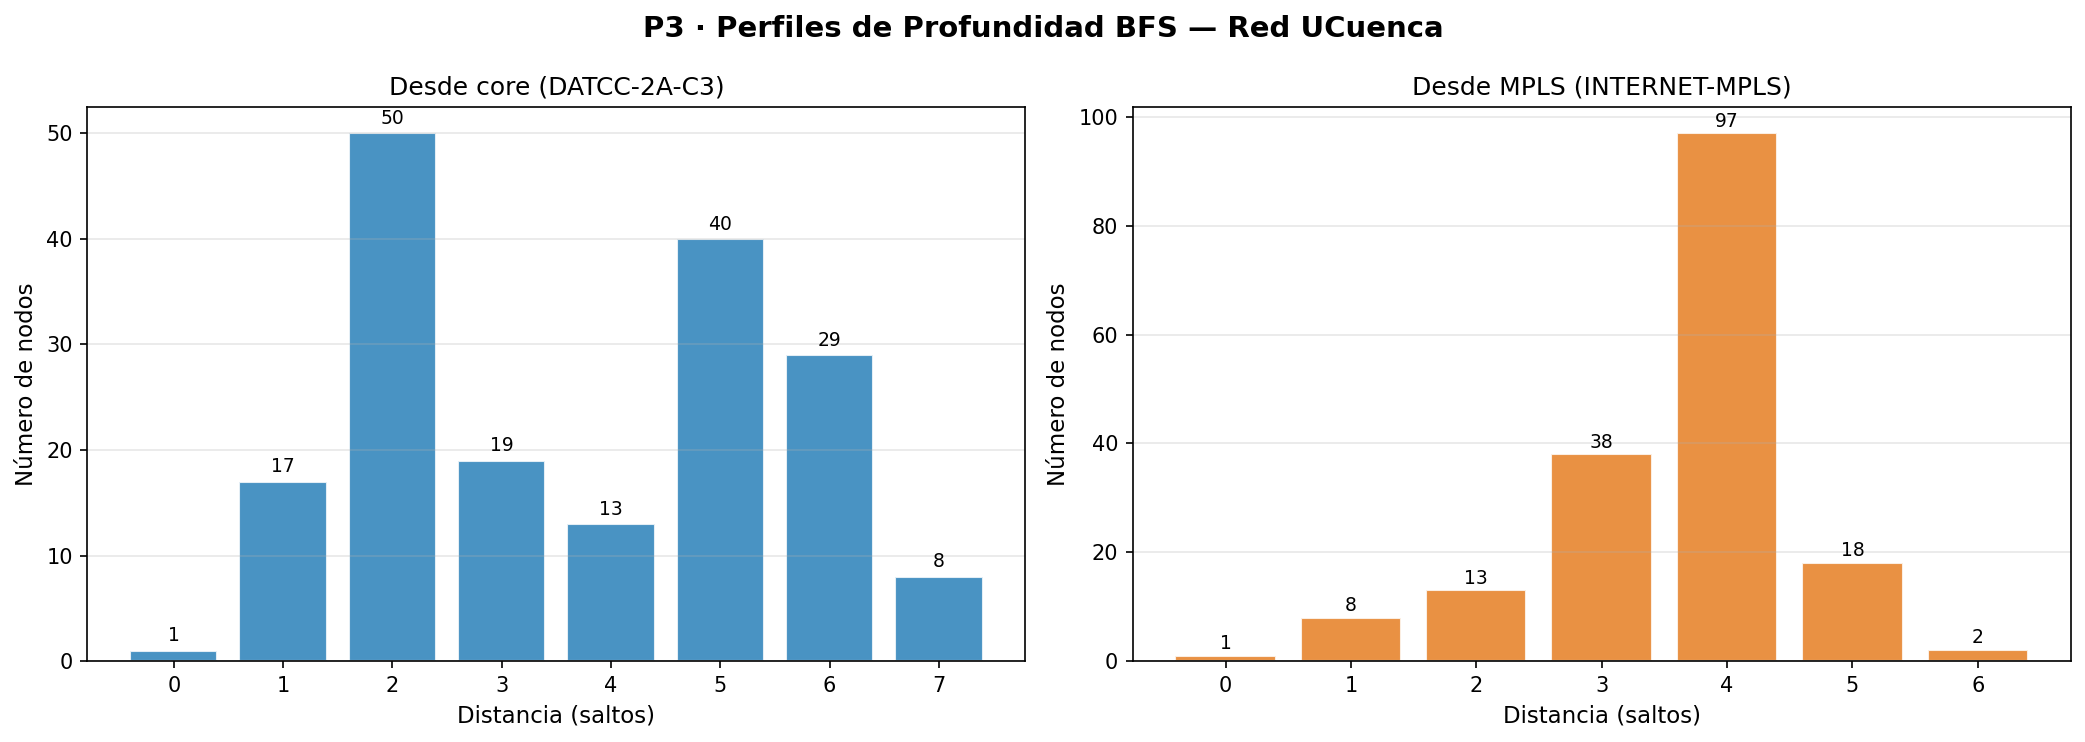
\includegraphics[width=0.8\linewidth]{images/p3_perfil_profundidad.png}
        \caption{Perfil de profundidad del BFS desde el core.}
        \label{fig:bfs}
    \end{subfigure}
    \vfill
    \begin{subfigure}[b]{0.7\linewidth}
        \centering
        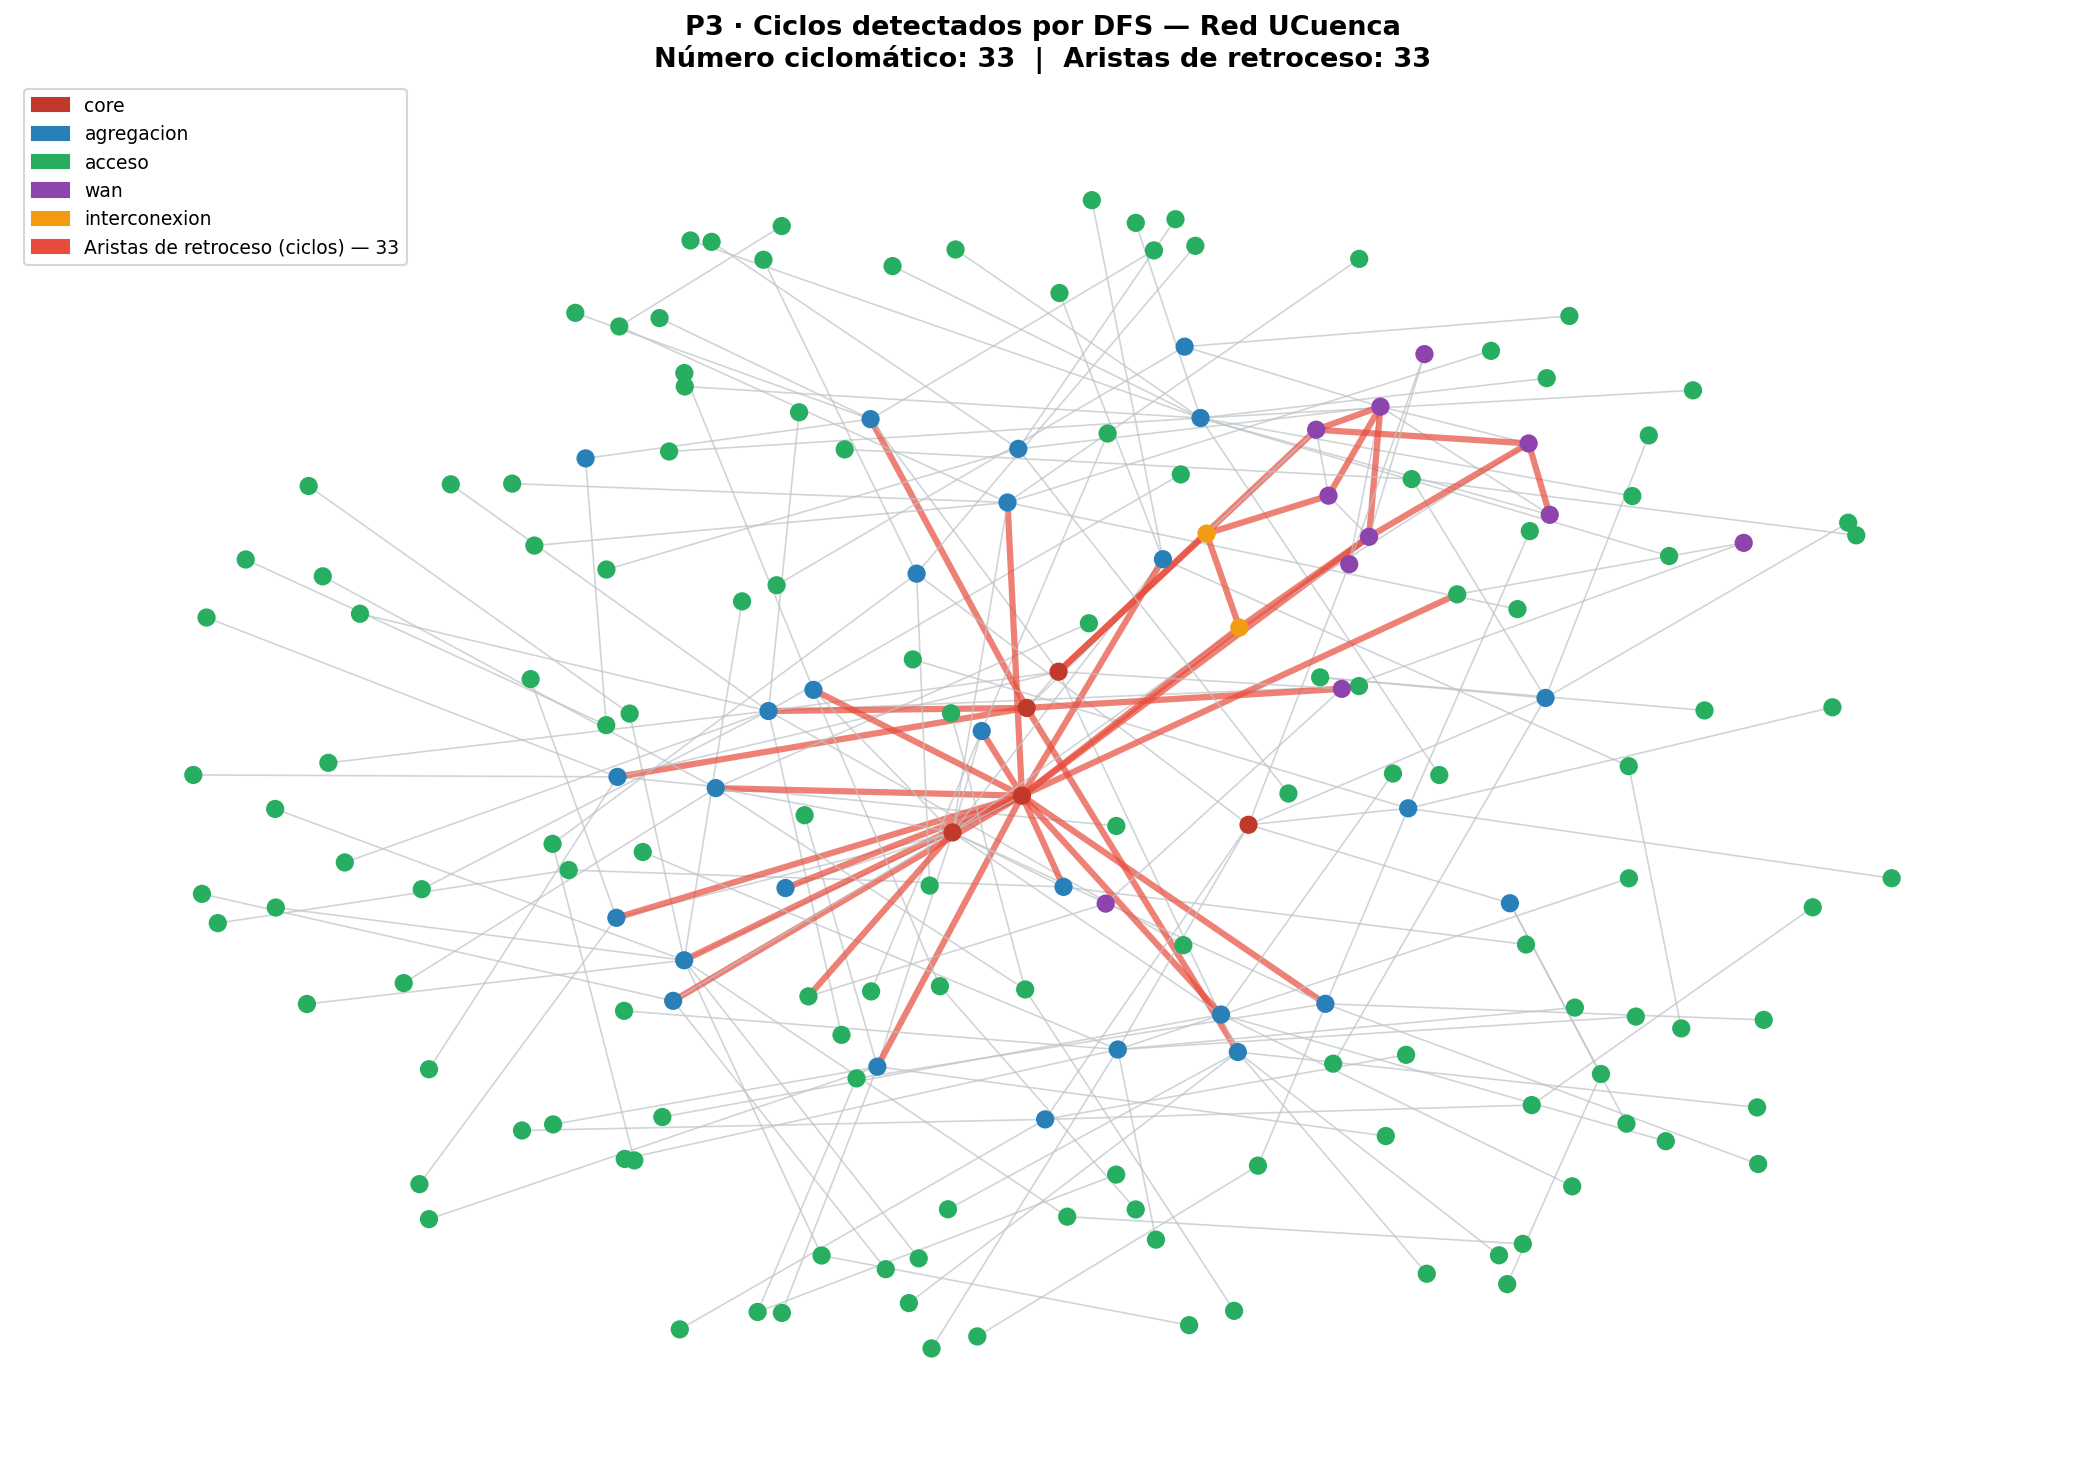
\includegraphics[width=\linewidth]{images/p3_ciclos.png}
        \caption{Ciclos detectados y su distribución por campus.}
        \label{fig:ciclos}
    \end{subfigure}
    \caption{Análisis de recorridos: BFS y ciclos de redundancia.}
    \label{fig:recorridos}
\end{figure}

La Figura~\ref{fig:recorridos}a muestra el perfil de profundidad del BFS
lanzado desde el nodo de mayor coreness (DATCC-2A-C3): la mayoría de los
nodos se encuentran a 4--7 saltos, confirmando el diámetro efectivo de la red.
La Figura~\ref{fig:recorridos}b presenta la distribución de los ciclos
detectados por DFS, coloreados por campus.

La descomposición \textit{k}-core revela que solo 5 nodos forman el 3-core
(los switches de core más INTERNET-MPLS), mientras que 132 nodos son hojas de
acceso (1-core).

El número ciclomático predice exactamente los ciclos existentes:
\[
  \mu = m - n + 1 = 209 - 177 + 1 = 33
\]
La Figura~\ref{fig:ciclos} confirma que los 33 ciclos detectados por DFS
coinciden con las 33 aristas de retroceso. Los ciclos se distribuyen por campus:
Central 21, Balzay 9, MPLS 3, y \textbf{cero ciclos en Paraíso, Yanuncay y
Hospitalidad} (árbol puro $\Rightarrow$ cualquier fallo aísla directamente los
equipos de acceso aguas abajo). Esto cierra el círculo con P1: los 141 puentes
son exactamente las aristas fuera de todo ciclo; los 68 no-puentes forman los
33 ciclos.

\subsection{Detección de comunidades}

La \textbf{modularidad} $Q$ mide la calidad de una partición en comunidades:
\[
  Q = \frac{1}{2m}\sum_{i,j}\left[A_{ij} - \frac{k_i k_j}{2m}\right]\delta(c_i, c_j)
\]
donde $A_{ij}$ es la entrada de la matriz de adyacencia, $k_i k_j/(2m)$ es
la fracción esperada de aristas entre $i$ y $j$ en el modelo nulo ER, y
$\delta(c_i,c_j)=1$ si los nodos pertenecen a la misma comunidad. $Q\in(-1,1]$;
valores $Q > 0.3$ se consideran estructura de comunidad significativa.

La \textbf{NMI} (Normalized Mutual Information) compara dos particiones:
\[
  \text{NMI}(X,Y) = \frac{2\,I(X;Y)}{H(X)+H(Y)} \in [0,1]
\]
donde $H(\cdot)$ es la entropía de Shannon de cada partición e $I(X;Y)$ su
información mutua. $\text{NMI}=1$ indica particiones idénticas.

\begin{figure}[H]
    \centering
    \begin{subfigure}[b]{0.48\linewidth}
        \centering
        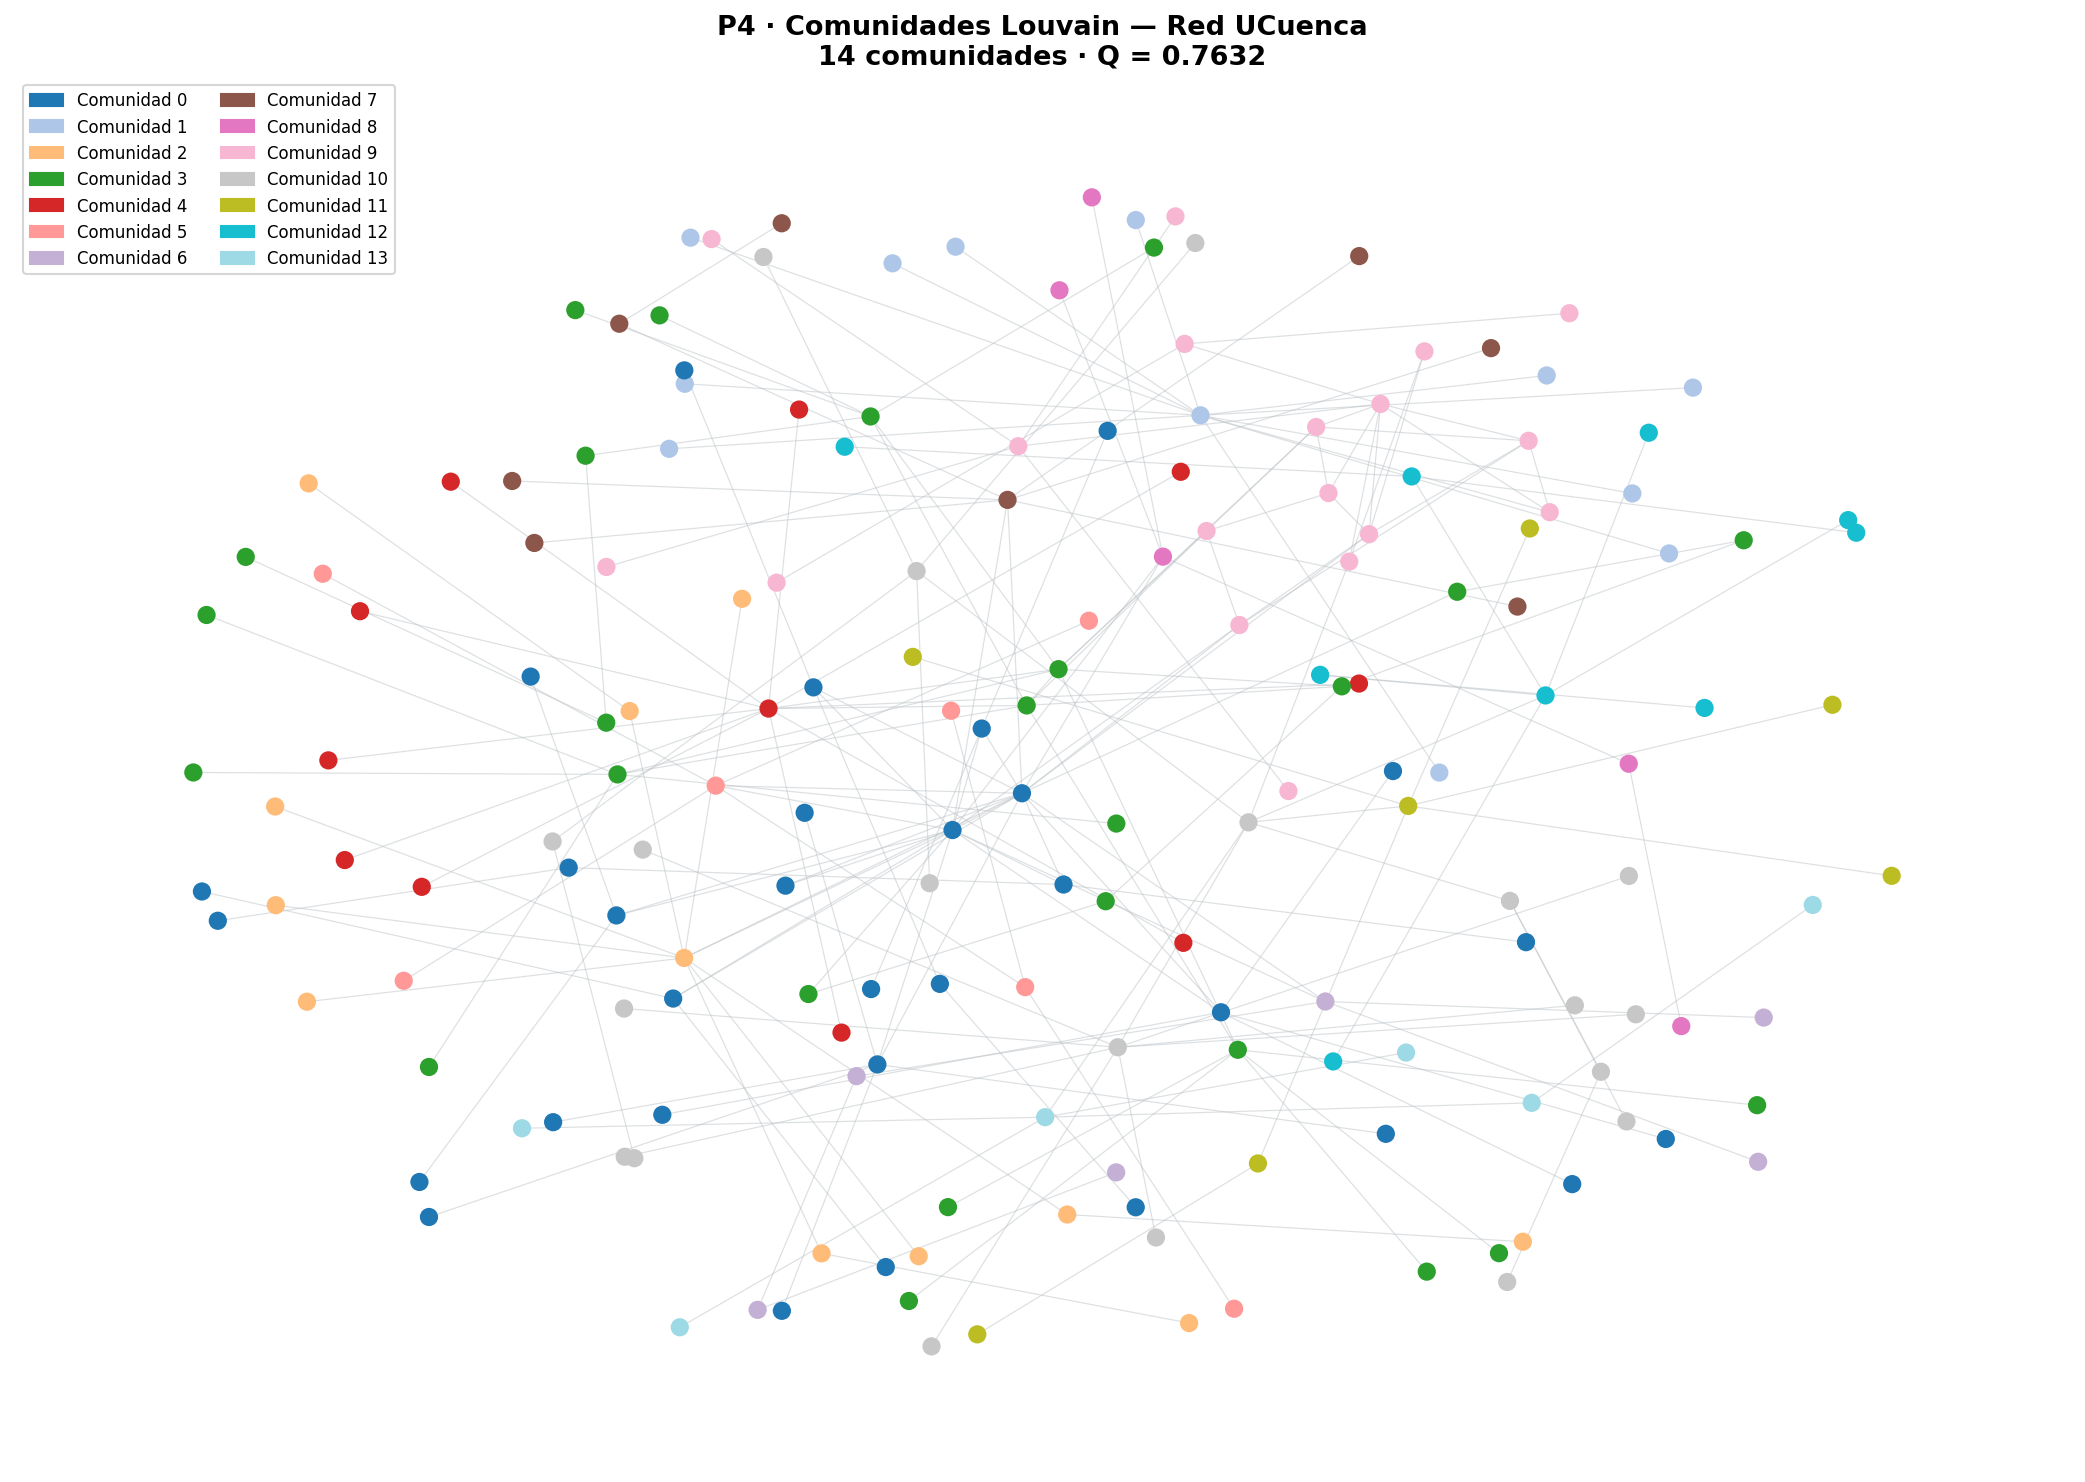
\includegraphics[width=\linewidth]{images/p4_comunidades_louvain.png}
        \caption{Comunidades Louvain ($Q=0.73$, 6 comunidades).}
        \label{fig:louvain}
    \end{subfigure}
    \hfill
    \begin{subfigure}[b]{0.48\linewidth}
        \centering
        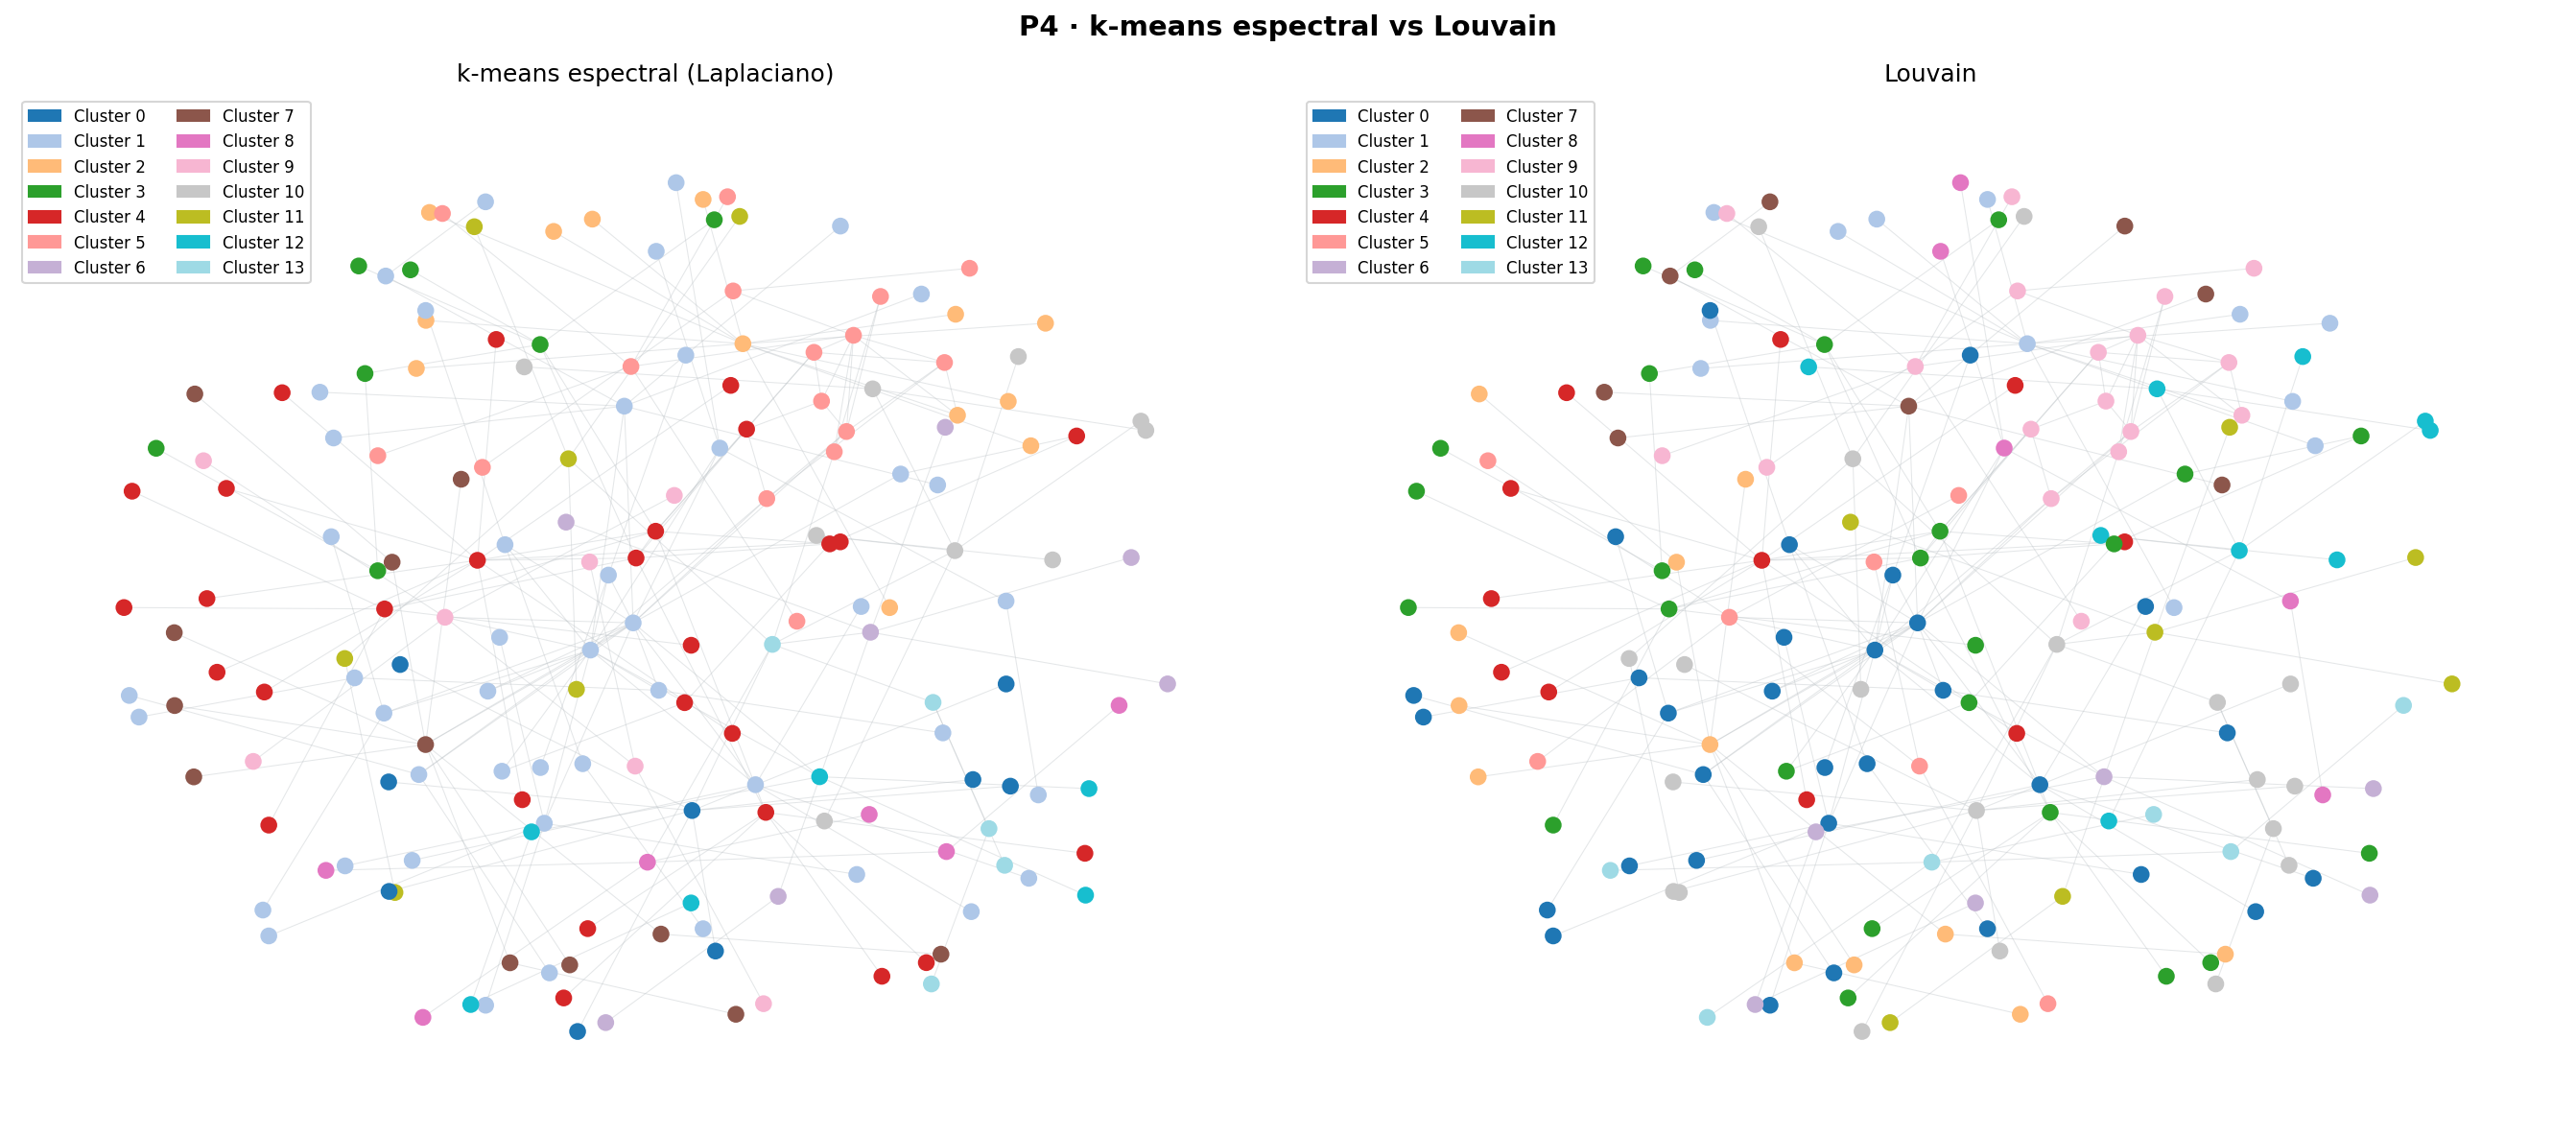
\includegraphics[width=\linewidth]{images/p4_kmeans_vs_louvain.png}
        \caption{Comparativa Louvain vs.\ k-means (NMI = 0.91).}
        \label{fig:kmeans_louvain}
    \end{subfigure}
    \caption{Detección de comunidades y comparación de métodos.}
    \label{fig:comunidades}
\end{figure}

\begin{figure}[H]
    \centering
    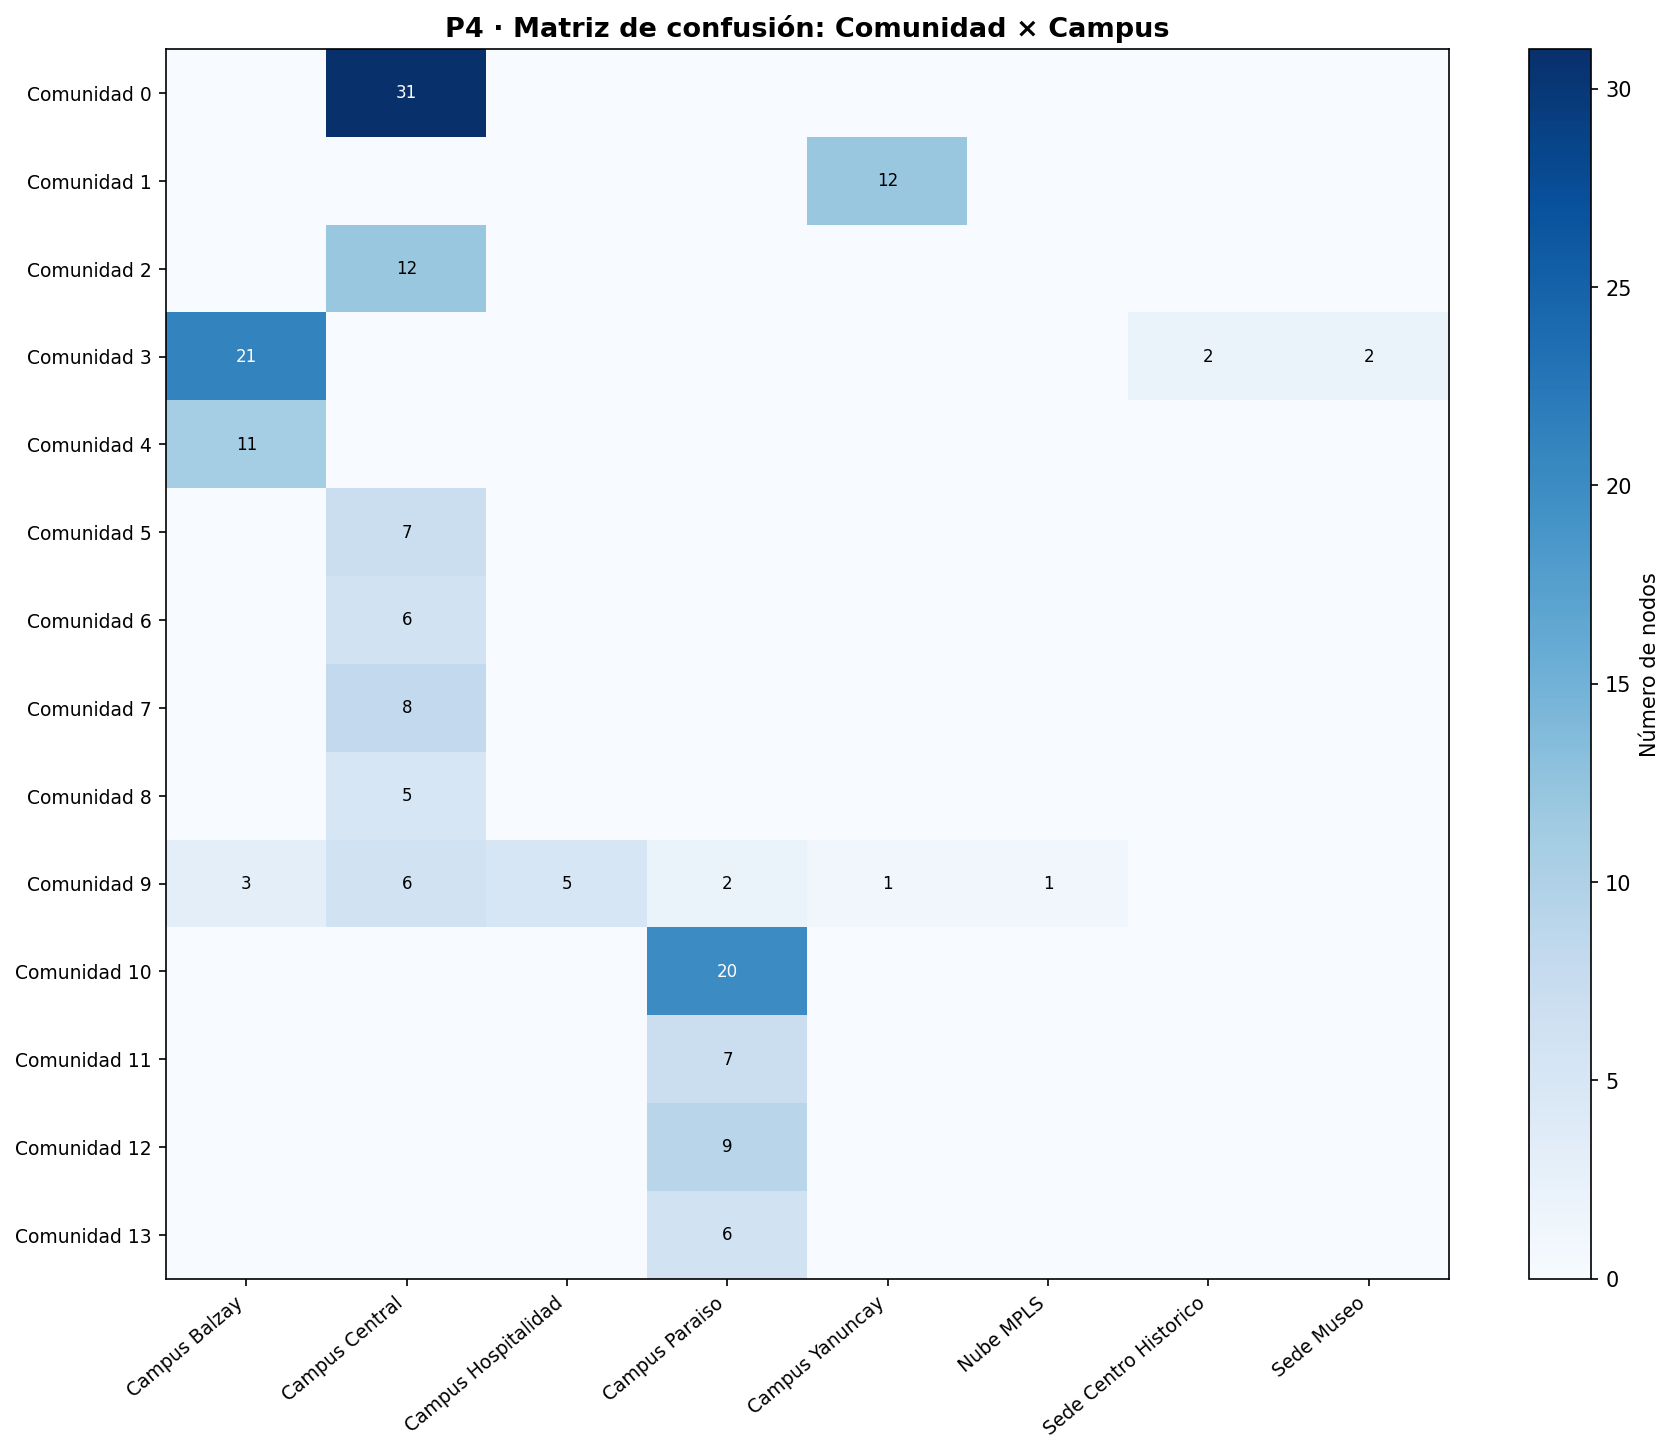
\includegraphics[width=0.7\linewidth]{images/p4_confusion_campus.png}
    \caption{Matriz de confusión: comunidades Louvain vs.\ campus reales.}
    \label{fig:confusion}
\end{figure}

La Figura~\ref{fig:comunidades}a presenta las 6 comunidades Louvain
superpuestas sobre el grafo, donde cada color corresponde a una comunidad
detectada. La Figura~\ref{fig:comunidades}b muestra la comparativa entre
la partición Louvain y el agrupamiento k-means aplicado sobre coordenadas
espectrales (NMI = 0.91 entre ambos métodos).

El algoritmo de Louvain detecta 6 comunidades con modularidad $Q = 0.73$,
valor alto que indica una separación clara entre grupos. La matriz de confusión
(Fig.~\ref{fig:confusion}) muestra una correspondencia casi perfecta
($> 95\%$) entre comunidades y campus físicos: la topología \textit{refleja
fielmente} la geografía universitaria. La NMI entre la partición Louvain y
los campus reales es 0.618, lo que indica alta correspondencia pero no
perfecta (algunos nodos de borde son asignados al campus vecino).

\begin{hallazgo}
\textbf{Hallazgo:} la alta modularidad ($Q=0.73$) tiene dos caras. Por un
lado, facilita la contención de fallos: un problema en el Campus Yanuncay
tiende a quedarse ahí. Por otro, implica que los routers inter-campus son
puentes críticos entre comunidades, y su falla aísla completamente un campus.
\end{hallazgo}

% ============================================================
%  6. OPTIMIZACIÓN — FASE 3
% ============================================================
\section{Optimización (Fase~3)}

\subsection{Caminos mínimos: Dijkstra y Floyd-Warshall}

El \textbf{camino mínimo} entre dos nodos $s,t$ es la secuencia de aristas
de menor peso total. Se usaron dos algoritmos complementarios:

\begin{itemize}
  \item \textbf{Dijkstra} (un origen, grafo con pesos $\geq 0$):
        complejidad $O\bigl((m+n)\log n\bigr)$ con cola de prioridad binaria.
        Óptimo para redes dispersas.
  \item \textbf{Floyd-Warshall} (todos los pares):
        $d^{(k)}_{ij} = \min\bigl(d^{(k-1)}_{ij},\; d^{(k-1)}_{ik}+d^{(k-1)}_{kj}\bigr)$
        con complejidad $O(n^3)$. Produce la matriz completa de distancias
        en un único recorrido.
\end{itemize}

Se implementaron Dijkstra desde cero (cola de prioridad manual) y
Floyd-Warshall para todos los pares. La Figura~\ref{fig:tiempos} muestra
los tiempos de ejecución en redes de tamaño creciente.

\begin{figure}[H]
    \centering
    \begin{subfigure}[b]{\linewidth}
        \centering
        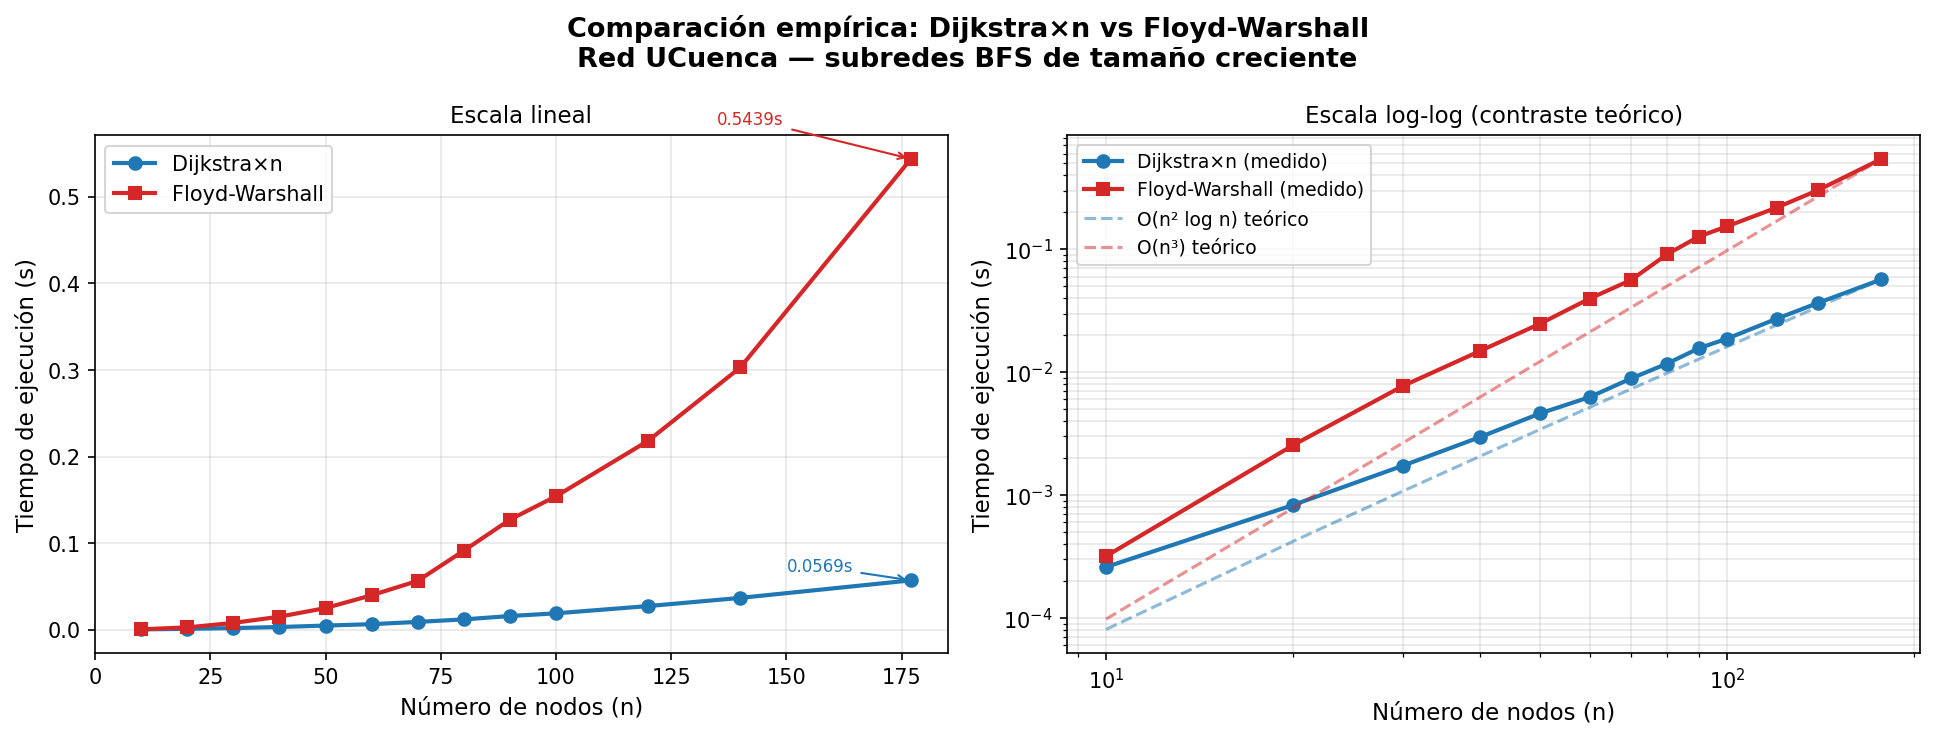
\includegraphics[width=\linewidth]{images/p5_tiempos_creciente.png}
        \caption{Tiempo de ejecución vs.\ tamaño de la red.}
        \label{fig:tiempos_creciente}
    \end{subfigure}
    \vfill
    
    \begin{subfigure}[b]{\linewidth}
        \centering
        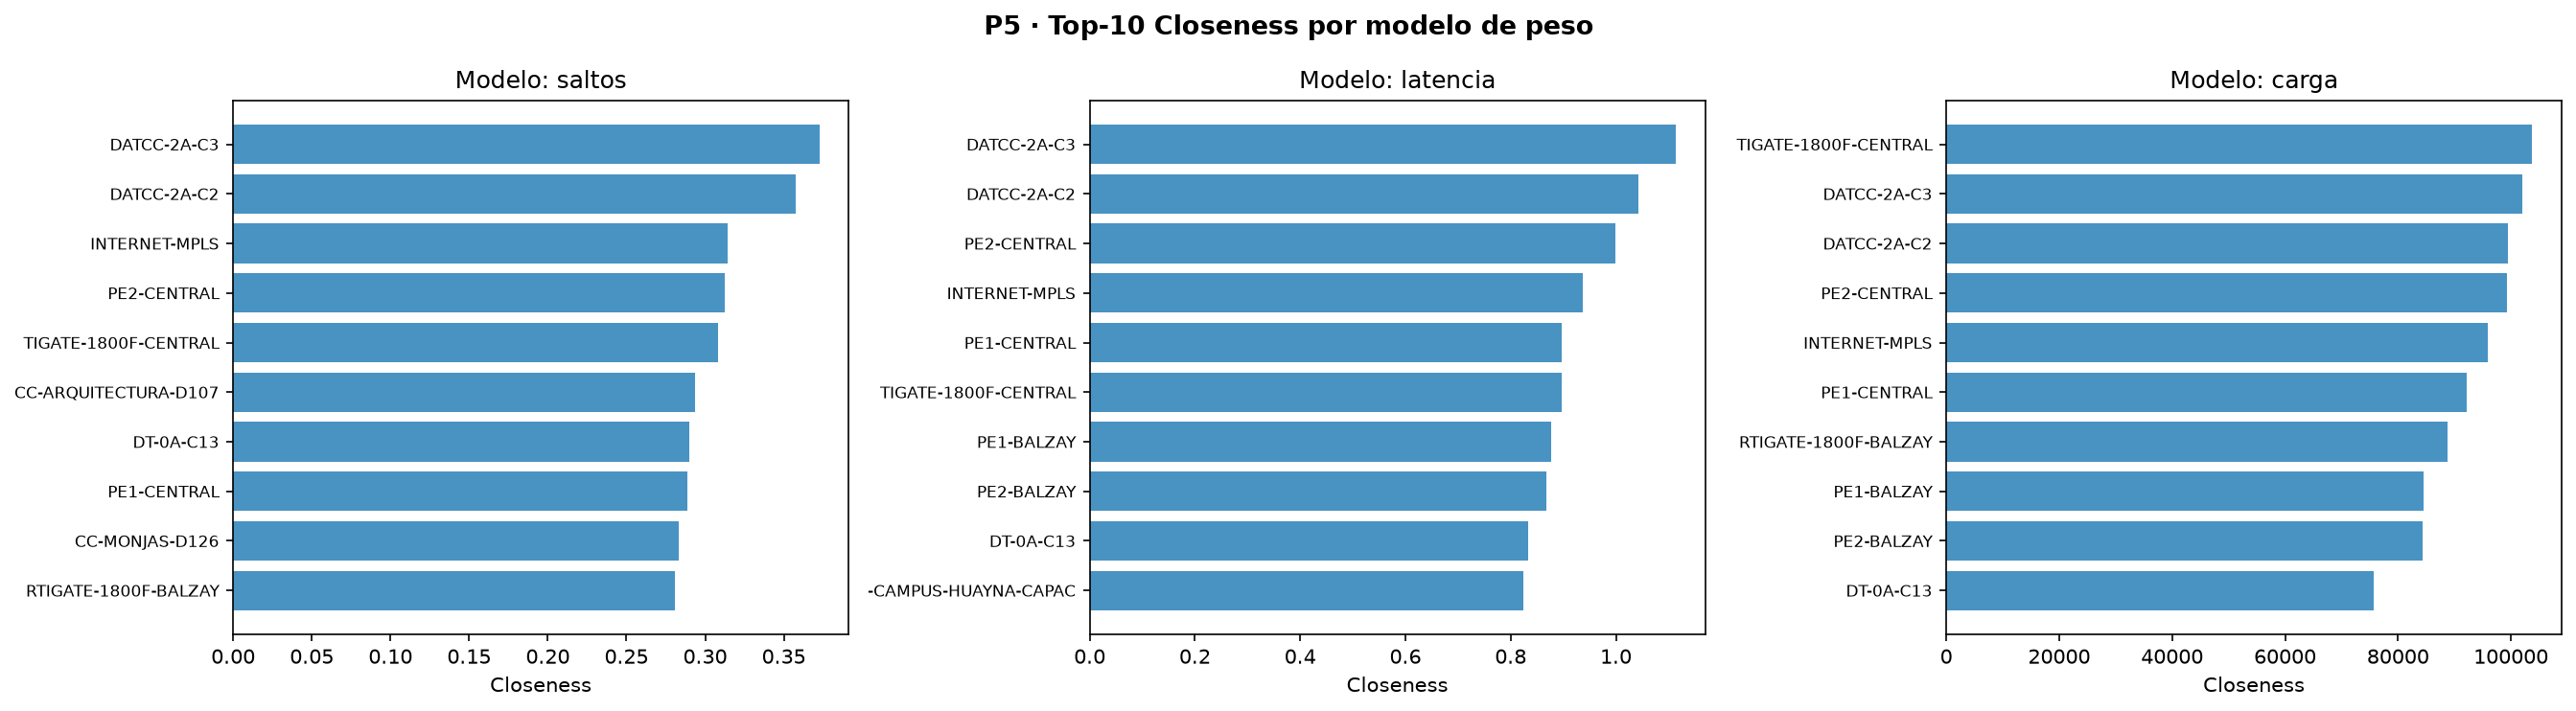
\includegraphics[width=\linewidth]{images/p5_closeness_comparativo.png}
        \caption{Closeness centrality: comparativa de métodos.}
        \label{fig:closeness}
    \end{subfigure}
    \caption{Análisis de caminos mínimos.}
    \label{fig:tiempos}
\end{figure}

La Figura~\ref{fig:tiempos}a compara el tiempo de ejecución de Dijkstra y
Floyd-Warshall sobre redes de tamaño creciente: Dijkstra escala linealmente
en el rango probado, mientras Floyd-Warshall crece cúbicamente y se vuelve
inviable para $n > 500$. La Figura~\ref{fig:tiempos}b muestra la closeness
centrality calculada con ambos métodos sobre la red UCuenca, confirmando
que producen resultados idénticos.

Dijkstra es $O((m + n)\log n)$ y es el algoritmo de elección para redes
dispersas como UCuenca. Floyd-Warshall ($O(n^3)$) resulta impractical para
$n > 500$ pero produce la matriz completa de distancias en un solo cálculo,
útil para métricas globales. El par más distante en la red es de 13 saltos
(nodo periférico de Campus Yanuncay~$\to$~nodo periférico de Campus Paraíso).

\subsection{Flujo máximo y corte mínimo}

El \textbf{flujo máximo} entre una fuente $s$ y un sumidero $t$ es:
\[
  f^* = \max_{f} \sum_{v:(s,v)\in E} f(s,v)
  \quad \text{s.t.} \quad
  f(u,v) \leq c(u,v),\;\; \sum_u f(u,v) = \sum_w f(v,w) \;\forall v \neq s,t
\]
El \textbf{Teorema de Ford-Fulkerson} establece que $f^* = $ capacidad del
\textit{corte mínimo}: el conjunto de aristas de menor capacidad total cuya
eliminación desconecta $s$ de $t$. Se compararon dos implementaciones:
\begin{itemize}
  \item \textbf{Ford-Fulkerson (DFS):} aumenta flujo por caminos hallados en
        profundidad; puede requerir muchas iteraciones si las capacidades son grandes.
  \item \textbf{Edmonds-Karp (BFS):} siempre elige el camino aumentante más
        corto; garantiza $O(nm^2)$ iteraciones independientemente de las capacidades.
\end{itemize}

\begin{figure}[H]
    \centering
    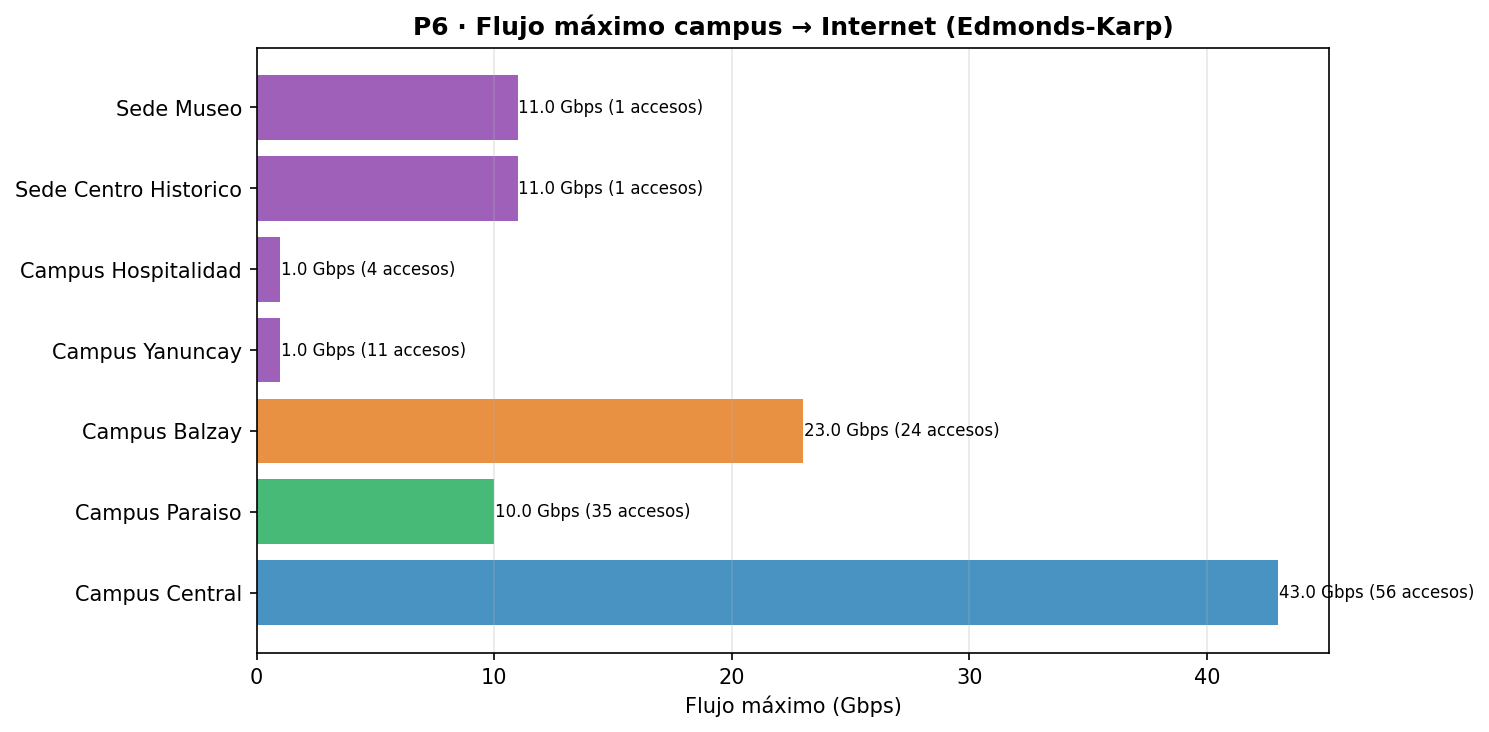
\includegraphics[width=0.7\linewidth]{images/p6_flujo_campus.png}
    \caption{Flujo máximo por campus hacia INTERNET-MPLS (Edmonds-Karp).}
    \label{fig:flujo_campus}
\end{figure}

\begin{table}[H]
\centering
\caption{Flujo máximo por campus. El corte mínimo identifica los cuellos de
         botella del backbone.}
\label{tab:flujo_campus}
\small
\begin{tabular}{L{4cm} C{3cm} C{3cm} C{3cm}}
    \toprule
    \encabezado{Campus} &
    \encabezado{Flujo máx. (Mbps)} &
    \encabezado{Long. media (saltos)} &
    \encabezado{Nodos acceso} \\
    \midrule
    \rowcolor{tabfila}
    Central         & 43\,000 & 6.3 & 56 \\
    Balzay          & 23\,000 & 5.6 & 24 \\
    \rowcolor{tabfila}
    C. Histórico    & 11\,000 & 5.0 & 1  \\
    Paraíso         & 10\,000 & 5.0 & 35 \\
    \rowcolor{tabfila}
    Yanuncay        & 1\,000  & 4.0 & 11 \\
    Hospitalidad    & 1\,000  & 3.0 & 4  \\
    \bottomrule
\end{tabular}
\end{table}

La Figura~\ref{fig:flujo_campus} muestra el flujo máximo calculado por
Edmonds-Karp desde cada campus hacia \texttt{INTERNET-MPLS}, con los
cuellos de botella marcados en rojo. La Tabla~\ref{tab:flujo_campus}
detalla el flujo máximo (Mbps), la longitud media del camino (saltos) y
el número de nodos de acceso por campus.

El corte mínimo del backbone pasa por \texttt{DATCC-2A-C3~$\to$~PE2-CENTRAL}
(20\,000 Mbps) y \texttt{DATCC-2A-C3~$\to$~FORTIGATE-1800F-CENTRAL}
(10\,000 Mbps). Campus Yanuncay tiene el flujo más limitado (1\,000 Mbps) por
el único enlace de su router de campus.

\textbf{Comparación Ford-Fulkerson vs Edmonds-Karp.} En la mayoría de campus
ambos algoritmos necesitan el mismo número de iteraciones (capacidades múltiplo
de 1\,000~Mbps, pocos caminos alternativos). En las sedes históricas,
Ford-Fulkerson (DFS) requiere 3 iteraciones y Edmonds-Karp (BFS) solo~2,
confirmando el lema de caminos aumentantes más cortos. El corte de Central
concentra capacidad en enlaces de alta velocidad; en Balzay el cuello está en
acceso; Paraíso, Yanuncay y Hospitalidad dependen de un único enlace de salida.

\textbf{Corte mínimo vs.\ puentes.} El corte mínimo identifica vulnerabilidad
de \textit{rendimiento} (capacidad); los puentes de P1 miden vulnerabilidad
\textit{estructural} (conectividad). No siempre coinciden: el corte de Central
incluye aristas de alta capacidad que no son puentes porque existen rutas
alternativas; la arista \texttt{CCJ-CJURIDICO-D4\,$\to$\,INTERNET-MPLS}
(1~Gbps) es simultáneamente corte mínimo \textit{y} puente en Campus Central.

\textbf{Comparación con flujo de costo mínimo.} El problema de flujo de costo
mínimo (MCF) para 5\,000 Mbps de demanda por campus produce rutas un 37\%
más cortas (3.80 saltos promedio vs.\ 5.96 de Edmonds-Karp), al redirigir el
tráfico por caminos con menos hops en lugar de maximizar el volumen total.

\subsection{Localización de instalaciones (colectores)}

Se formularon dos modelos de localización de instalaciones sobre el grafo:

\textbf{\textit{p}-Mediana} — minimiza la suma ponderada de distancias al
colector más cercano:
\[
  \min_{S\subseteq V,\,|S|=p} \sum_{v \in V} \min_{s \in S} d(v,s)
\]

\textbf{\textit{p}-Centro} — minimiza la distancia máxima (radio de cobertura):
\[
  \min_{S\subseteq V,\,|S|=p} \max_{v \in V} \min_{s \in S} d(v,s)
\]
Ambos son NP-difíciles en general; se compararon una \textbf{heurística voraz}
(añade iterativamente el nodo que más reduce el objetivo) con un
\textbf{solver exacto} de programación entera mixta (PuLP/CBC con
formulación de localización-asignación).

Se resolvieron los modelos de \textit{p}-Mediana (minimiza suma de distancias)
y \textit{p}-Centro (minimiza la distancia máxima) para $p \in \{1,2,3,5\}$,
con dos enfoques: heurística voraz y solver exacto de programación entera (PuLP/CBC).

\begin{figure}[H]
    \centering
    \begin{subfigure}[b]{0.8\linewidth}
        \centering
        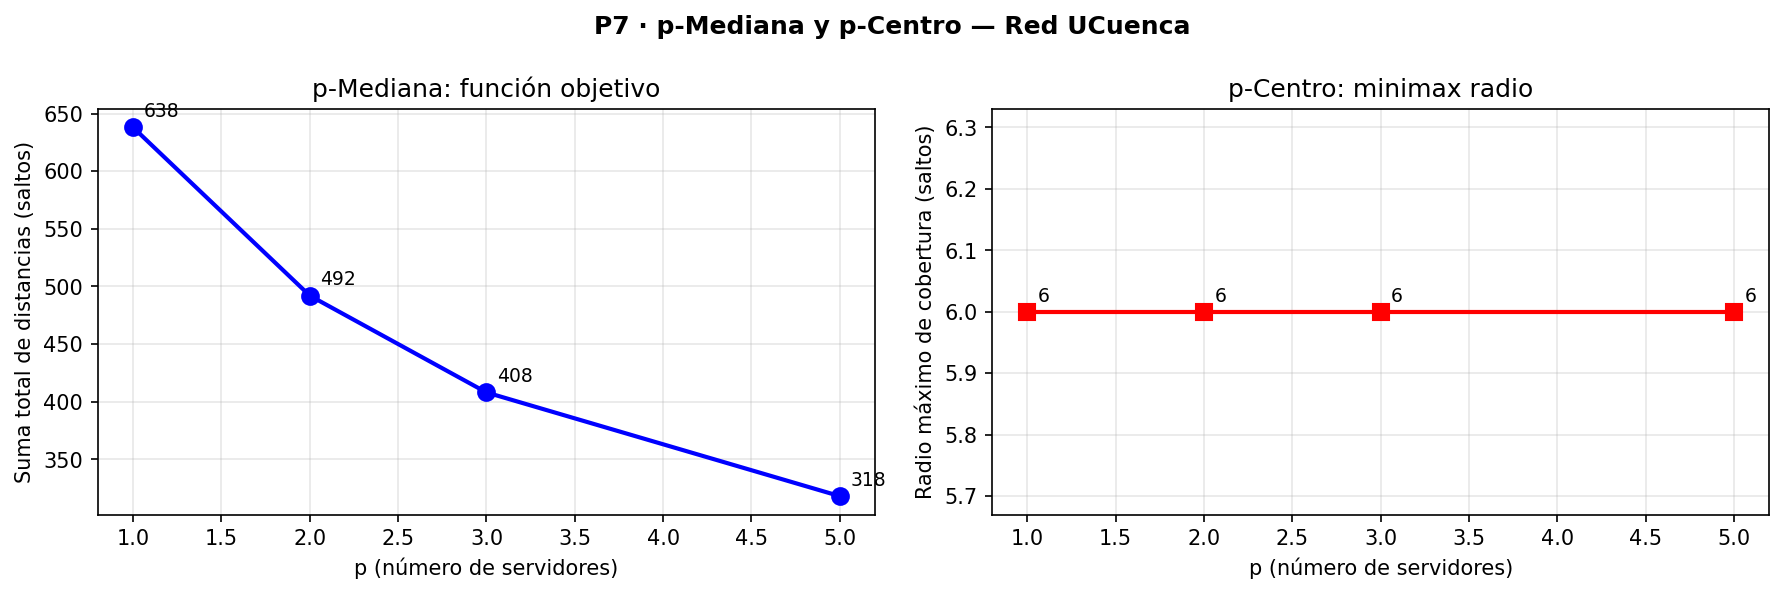
\includegraphics[width=\linewidth]{images/p7_mediana_vs_centro.png}
        \caption{Comparativa heurística: \textit{p}-Mediana vs.\ \textit{p}-Centro.}
        \label{fig:mediana_centro}
    \end{subfigure}
    \vfill
    \begin{subfigure}[b]{0.8\linewidth}
        \centering
        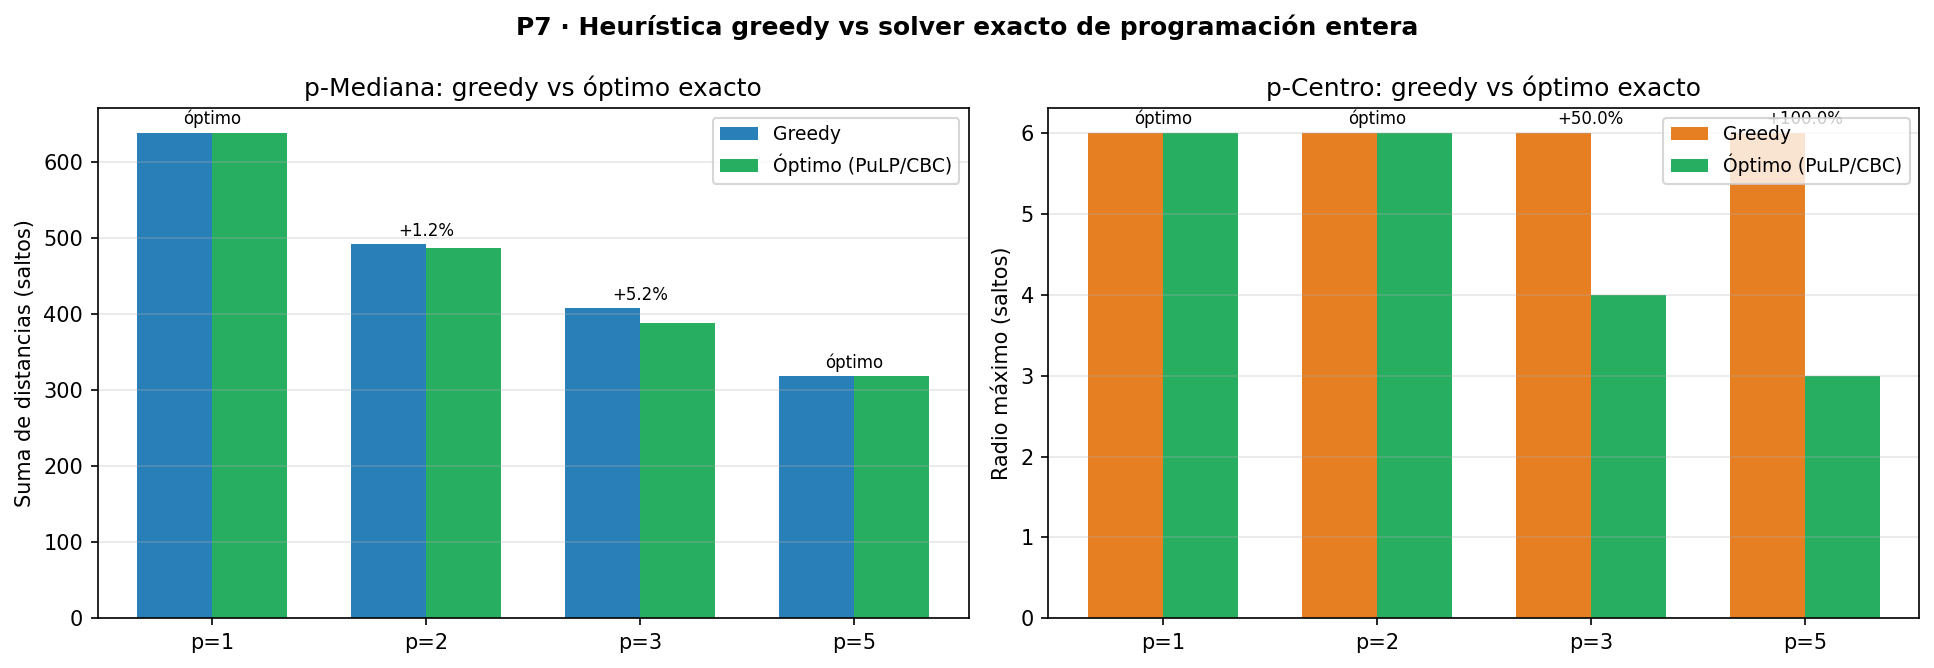
\includegraphics[width=\linewidth]{images/p7_heuristica_vs_solver.png}
        \caption{Gap heurística vs.\ solver exacto por valor de $p$.}
        \label{fig:heuristica_solver}
    \end{subfigure}
    \caption{Localización de instalaciones: modelos y comparativa de métodos.}
    \label{fig:localizacion}
\end{figure}

La Figura~\ref{fig:localizacion}a compara la solución heurística voraz con
la solución exacta para \textit{p}-Mediana y \textit{p}-Centro en $p \in
\{1,2,3,5\}$: las barras muestran el coste (suma de distancias / radio
máximo) de cada método. La Figura~\ref{fig:localizacion}b grafica el
\textit{gap} porcentual heurística vs.\ solver exacto, poniendo en evidencia
el colapso del greedy para \textit{p}-Centro con $p \geq 3$.

Para $p=3$, la heurística voraz selecciona \texttt{INTERNET-MPLS},
\texttt{DATCC-2A-C3} y \texttt{CPAR-C10} ---los tres nodos de mayor
betweenness y closeness--- confirmando que el diagnóstico de centralidad
y la optimización convergen en los mismos nodos críticos.

\begin{aviso}
\textbf{Hallazgo metodológico clave (\textit{p}-Centro):} para
\textit{p}-Mediana el greedy es casi óptimo (gap $\leq 5\%$: 0\%, 1.23\%,
5.15\%, 0\% en $p=1,2,3,5$). Para \textit{p}-Centro, el greedy se estanca
en radio~6 desde $p=1$ y nunca mejora (gaps: 0\%, 0\%, \textbf{50\%},
\textbf{100\%}), mientras el solver exacto baja a radio~4 ($p=3$) y radio~3
($p=5$). La razón: el greedy añade el nodo que reduce el radio actual, pero
sin visibilidad de que \textit{reubicar} un centro existente destrabaría la
cota. Conclusión: para \textit{p}-Centro con $p\geq 3$ el greedy no es
confiable y se requiere solver exacto (PuLP/CBC).
\end{aviso}

% ============================================================
%  7. ROBUSTEZ — FASE 4
% ============================================================}
\section{Robustez (Fase~4)}

\subsection{Percolación de nodos: la paradoja de la robustez}

La \textbf{percolación de nodos} modela la degradación progresiva de una red
bajo eliminación secuencial de nodos. Dado que se elimina una fracción $f$
de los nodos, se mide el tamaño relativo de la \textbf{componente gigante}
(componente conexa más grande):
\[
  S(f) = \frac{|\text{componente gigante tras eliminar } f \cdot n \text{ nodos}|}{n}
\]
El \textbf{umbral de percolación} $f_c$ es la fracción mínima de nodos cuya
eliminación colapsa la componente gigante ($S(f_c) < 5\%$). Para una red
libre de escala con $2 < \alpha < 3$, la teoría predice $f_c \to 1$ bajo
fallos aleatorios (robustez alta) pero $f_c \ll 1$ bajo ataques dirigidos a hubs.

Se simularon cuatro estrategias de eliminación de nodos y se midió la
fracción del tamaño de la componente gigante $S(f)$.

\begin{figure}[H]
    \centering
    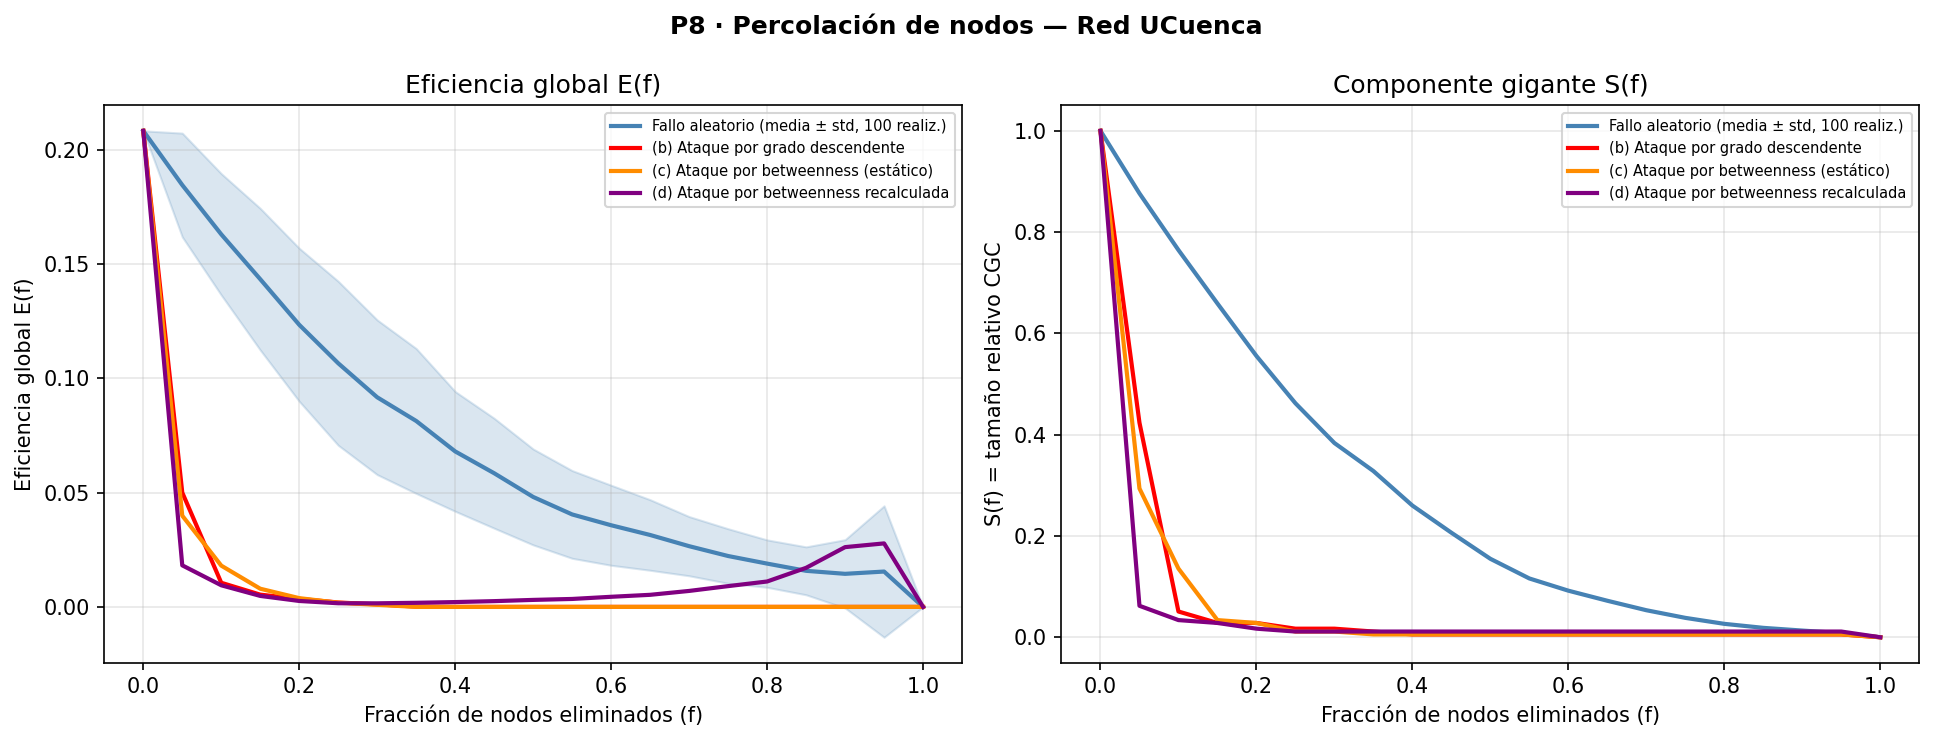
\includegraphics[width=0.8\linewidth]{images/p8_robustez_nodos.png}
    \caption{Curvas de robustez $S(f)$ bajo cuatro estrategias de ataque
             (100 realizaciones con banda de desviación estándar para la
             estrategia aleatoria).}
    \label{fig:robustez_nodos}
\end{figure}

\begin{table}[H]
\centering
\caption{Umbral de colapso $f_c$ ($S < 5\%$) por estrategia.}
\label{tab:percolacion}
\small
\begin{tabular}{L{5.5cm} C{2.5cm} L{5cm}}
    \toprule
    \encabezado{Estrategia} &
    \encabezado{$f_c$} &
    \encabezado{Interpretación} \\
    \midrule
    \rowcolor{tabfila}
    (a) Aleatoria (100 realizaciones) & 0.75  & Red muy robusta \\
    (b) Por grado (estático)          & 0.15  & Frágil \\
    \rowcolor{tabfila}
    (c) Por betweenness (estático)    & 0.15  & Frágil \\
    (d) Betweenness recalculado       & 0.10  & Muy frágil \\
    \bottomrule
\end{tabular}
\end{table}

La Figura~\ref{fig:robustez_nodos} presenta las cuatro curvas $S(f)$: la
estrategia aleatoria (banda sombreada para 100 realizaciones) desciende
muy lentamente, mientras que las estrategias dirigidas colapsan la
componente gigante con una fracción $f$ mucho menor. La Tabla~\ref{tab:percolacion}
resume el umbral de colapso $f_c$ y su interpretación operativa para cada estrategia.

La ratio $\fc^{\text{aleatorio}} / \fc^{\text{ataque}} = 7.5$ es la
\textbf{paradoja de la robustez}: la misma propiedad de ley de potencia que
hace a la red resiliente ante fallos aleatorios la hace extremadamente
vulnerable ante ataques inteligentes. La estrategia (d) es la más efectiva
porque al recalcular el betweenness después de cada eliminación, el atacante
puede identificar los nuevos cuellos de botella que emergen tras cada caída.

\begin{hallazgo}
\textbf{Implicación operativa:} un atacante que calcule betweenness puede
colapsar la red comprometiendo \textbf{solo 18 dispositivos (10\%)} con la
estrategia recalculada, donde cada compromiso revela el siguiente objetivo.
El plan de respuesta debe priorizar \textit{detección temprana} en los nodos
críticos (DATCC-2A-C3, CPAR-C10, INTERNET-MPLS) y \textit{aislamiento rápido}
antes que recuperación, para evitar que un hub comprometido sirva de pivote.
\end{hallazgo}

\subsection{Percolación de aristas}

La \textbf{percolación de aristas} es análoga a la de nodos pero elimina
aristas en lugar de nodos. La fracción de aristas eliminadas es $q$, y se
mide igualmente $S(q)$. El \textbf{umbral de percolación de aristas}
$q_c$ para un grafo aleatorio con grado medio $\langle k \rangle$ es:
\[
  q_c = 1 - \frac{1}{\langle k \rangle - 1}
\]
Para redes de infraestructura con alta fracción de puentes, eliminar aristas
puente fragmenta la red directamente; en cambio, eliminar aristas en ciclos
no afecta la conectividad (son redundantes por definición).

\begin{figure}[H]
    \centering
    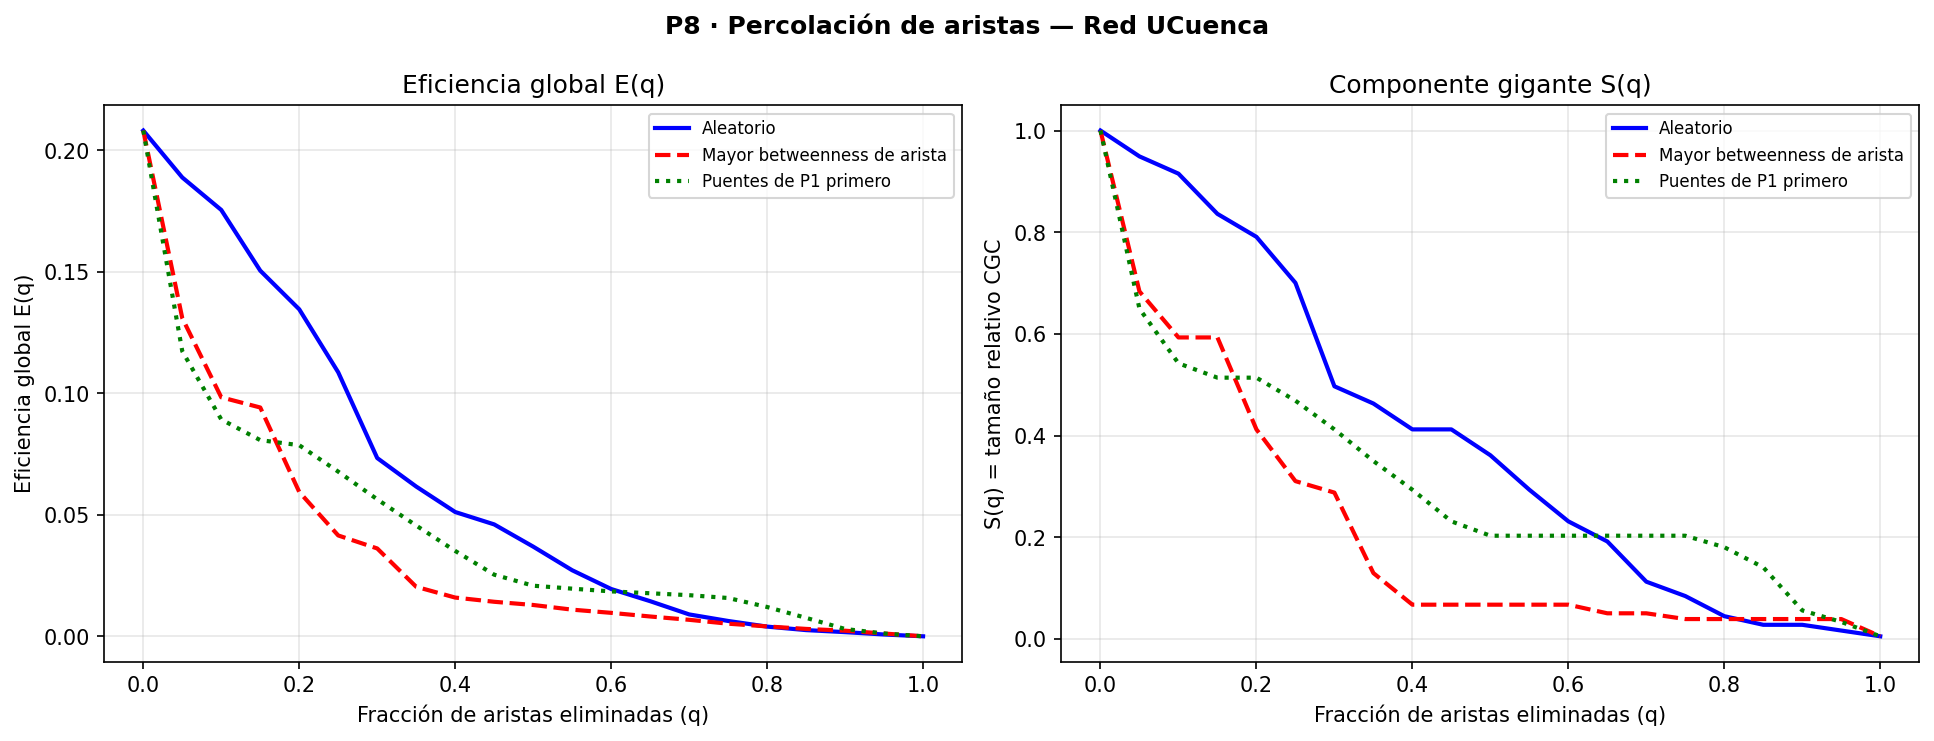
\includegraphics[width=\linewidth]{images/p8_robustez_aristas.png}
    \caption{Robustez bajo eliminación de aristas: aleatoria, por
             betweenness de arista, y ataque a puentes primero.}
    \label{fig:robustez_aristas}
\end{figure}

La Figura~\ref{fig:robustez_aristas} compara tres estrategias de eliminación
de aristas: aleatoria, por betweenness de arista (las aristas más cargadas
primero) y el ataque \textit{puentes primero}.

El ataque \textit{puentes primero} (eliminar los 141 puentes ordenados por
betweenness de arista antes de pasar a aristas arbitrarias) produce el mayor
daño: los puentes son por definición aristas no redundantes, y su eliminación
fragmenta la red de forma irreversible.

\subsection{Cascadas de carga (modelo Motter-Lai)}

El \textbf{modelo de Motter-Lai} (2002) formaliza las fallas en cascada por
sobrecarga. Cada nodo $i$ tiene:
\begin{align*}
  L_i(t) &= B_i(t) && \text{(carga = betweenness en el instante } t\text{)} \\
  C_i     &= (1+\alpha)\,L_i(0) && \text{(capacidad = }(1+\alpha)\times\text{ carga inicial)}
\end{align*}
donde $\alpha \geq 0$ es la \textbf{tolerancia}. Un nodo $i$ falla en $t+1$
si $L_i(t) > C_i$. Al fallar, sus caminos se reroutan por los nodos
restantes, aumentando la carga de los vecinos y pudiendo desencadenar
nuevas fallas (\textit{efecto dominó}).

El modelo asigna a cada nodo $i$ una carga $L_i = B_i$ (betweenness) y una
capacidad $C_i = (1+\alpha) \cdot L_i$. Al fallar un nodo, el betweenness se
redistribuye y puede superar la capacidad de vecinos, desencadenando cascadas.

\begin{figure}[H]
    \centering
    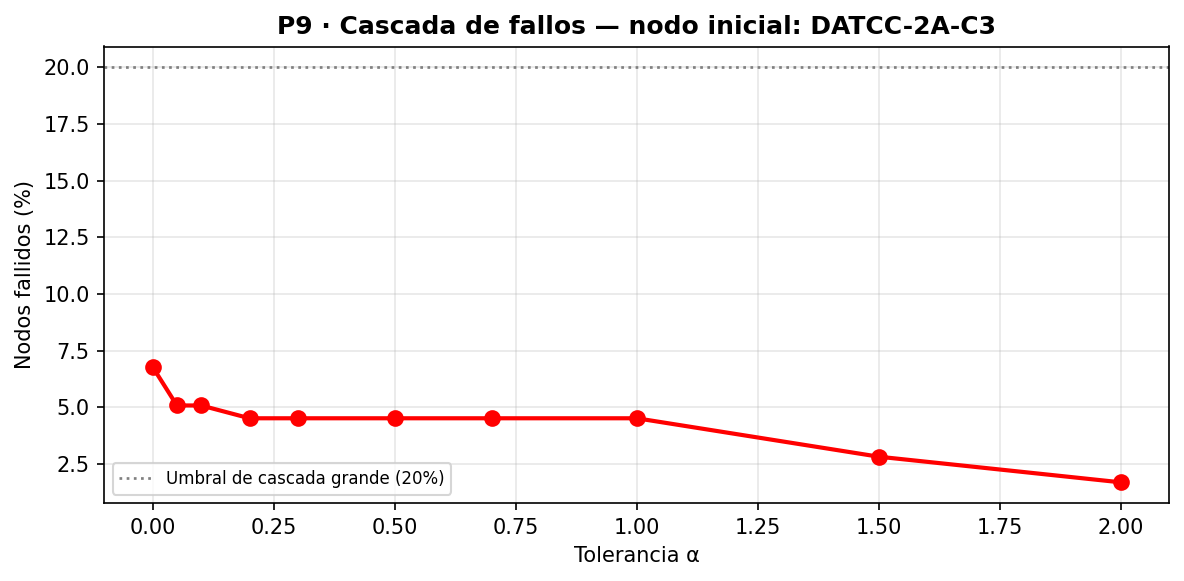
\includegraphics[width=0.75\linewidth]{images/p9_cascada.png}
    \caption{Fracción de nodos fallidos en cascada vs.\ tolerancia $\alpha$
             (nodo inicial: DATCC-2A-C3).}
    \label{fig:cascada}
\end{figure}

La Figura~\ref{fig:cascada} traza la fracción de nodos que fallan en cascada
en función del parámetro de tolerancia $\alpha$, iniciando la falla desde
el nodo más cargado (\texttt{DATCC-2A-C3}).

La Figura~\ref{fig:margen_critico} muestra el margen de tolerancia mínimo
$\alpha^*$ que cada nodo necesita para no propagar la cascada cuando falla,
identificando los equipos con menor margen de seguridad.

\begin{figure}[H]
    \centering
    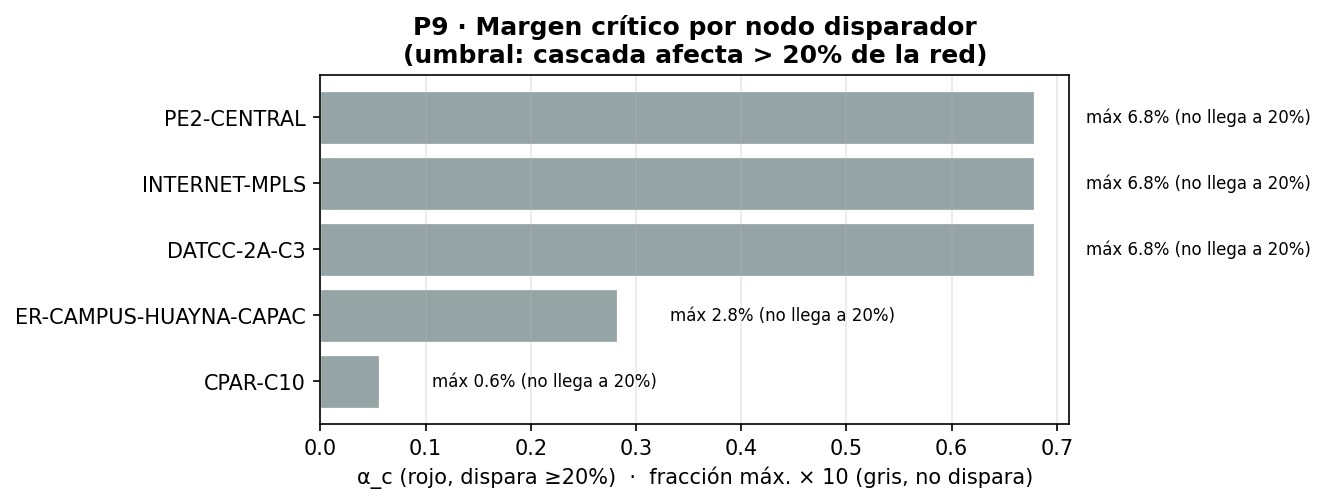
\includegraphics[width=0.75\linewidth]{images/p9_margen_critico.png}
    \caption{Margen crítico de tolerancia $\alpha^*$ por nodo: equipos con
             $\alpha^*$ pequeño son los más vulnerables a propagar cascadas
             incluso con baja sobrecarga.}
    \label{fig:margen_critico}
\end{figure}

La cascada máxima (12 nodos, $6.8\%$) ocurre en $\alpha = 0$; con
$\alpha \geq 0.3$ cae a menos del 5\%, y con $\alpha \geq 1.5$ se limita
a 5 nodos (2.8\%). \textbf{No existe un umbral $\tau_c$} para la red UCuenca:
la cascada nunca supera el $20\%$ incluso en el peor caso ($\alpha = 0$),
a diferencia de redes de potencia donde puede afectar el $100\%$.

\subsection{Modelo SIR y umbral epidémico}

El modelo \textbf{SIR} divide la población de nodos en tres compartimentos:
Susceptible ($S$), Infectado ($I$) y Recuperado ($R$). Las ecuaciones
diferenciales de campo medio son:
\begin{align*}
  \frac{dS}{dt} &= -\beta \langle k \rangle \frac{SI}{n} \\[3pt]
  \frac{dI}{dt} &= \beta \langle k \rangle \frac{SI}{n} - \gamma I \\[3pt]
  \frac{dR}{dt} &= \gamma I
\end{align*}
donde $\beta$ es la tasa de transmisión por enlace y $\gamma$ la tasa de
recuperación. El \textbf{umbral epidémico} $\tau_c$ separa el régimen
sub-crítico (la infección se extingue) del supra-crítico (epidemia global):
\[
  \tau_c = \frac{\beta_c}{\gamma} = \frac{\langle k \rangle}{\langle k^2 \rangle}
\]
Para redes heterogéneas con $\langle k^2 \rangle \gg \langle k \rangle$
(hubs), $\tau_c \to 0$: la red es intrínsecamente vulnerable a propagación.

\begin{figure}[H]
    \centering
    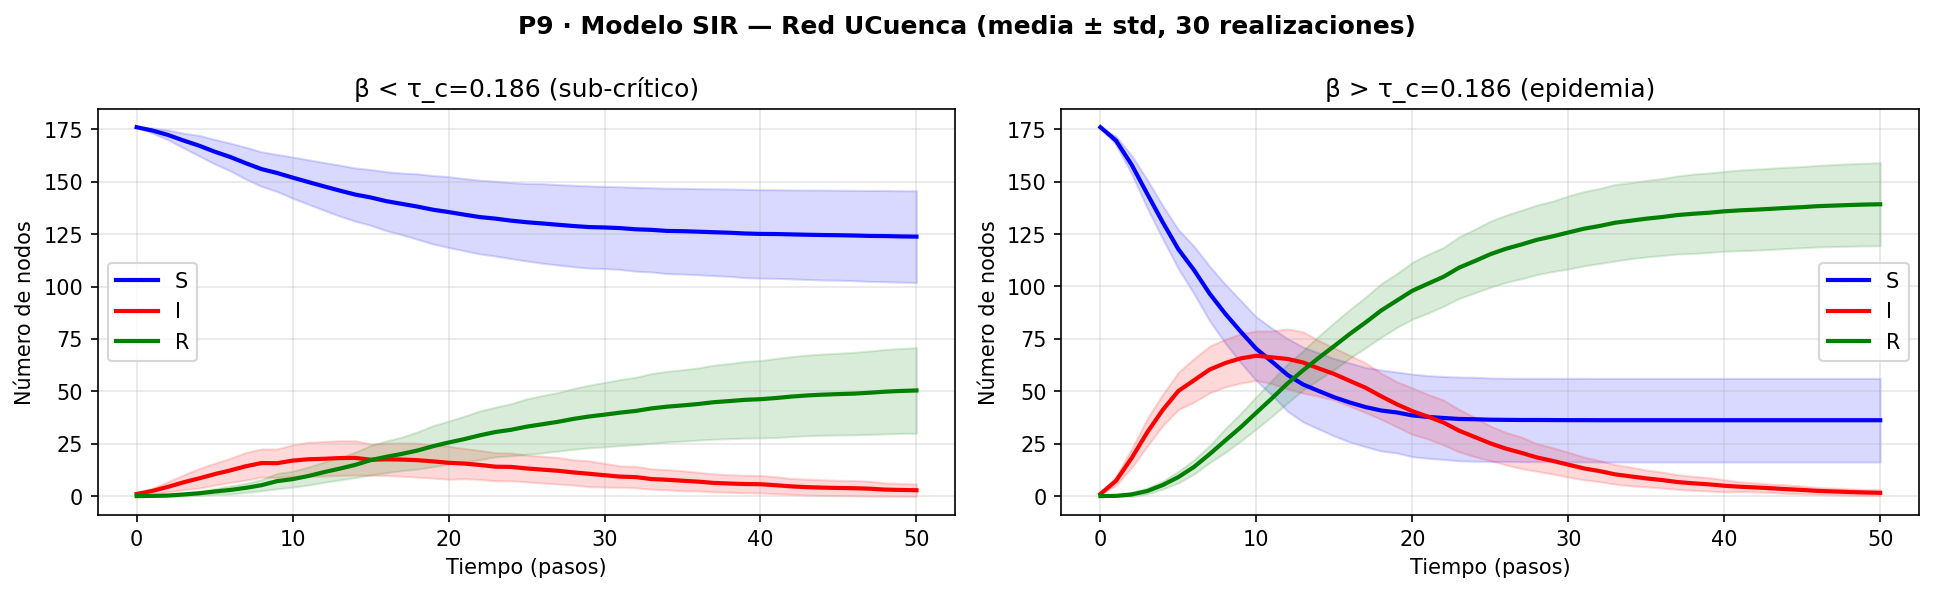
\includegraphics[width=\linewidth]{images/p9_sir.png}
    \caption{Evolución SIR: caso sub-crítico ($\beta = 0.093$) y
             sobre-crítico ($\beta = 0.372$), con $\gamma = 0.1$.}
    \label{fig:sir}
\end{figure}

La Figura~\ref{fig:sir} muestra la evolución temporal de los compartimentos
$S(t)$, $I(t)$ y $R(t)$ para dos valores de $\beta$: el caso sub-crítico
($\beta = 0.093 < \tau_c \gamma$) donde la infección se extingue en pocas
iteraciones, y el caso sobre-crítico ($\beta = 0.372$) donde el contagio
alcanza al $79\%$ de la red.

El umbral teórico de campo medio es:
\begin{equation}
    \tau_c = \frac{\prom{k}}{\prom{k^2}} = \frac{2.362}{12.694} = 0.1861
    \label{eq:tau_c}
\end{equation}

donde $\prom{k^2}$ es grande porque los hubs (switches de core con $k=17$)
inflan el promedio cuadrático. Un valor $\tau_c$ pequeño significa que la red
es \textbf{vulnerable a virus de baja contagiosidad}: cualquier malware con
tasa de propagación superior al $18.6\%$ por interfaz puede convertirse en
epidemia global.

\begin{figure}[H]
    \centering
    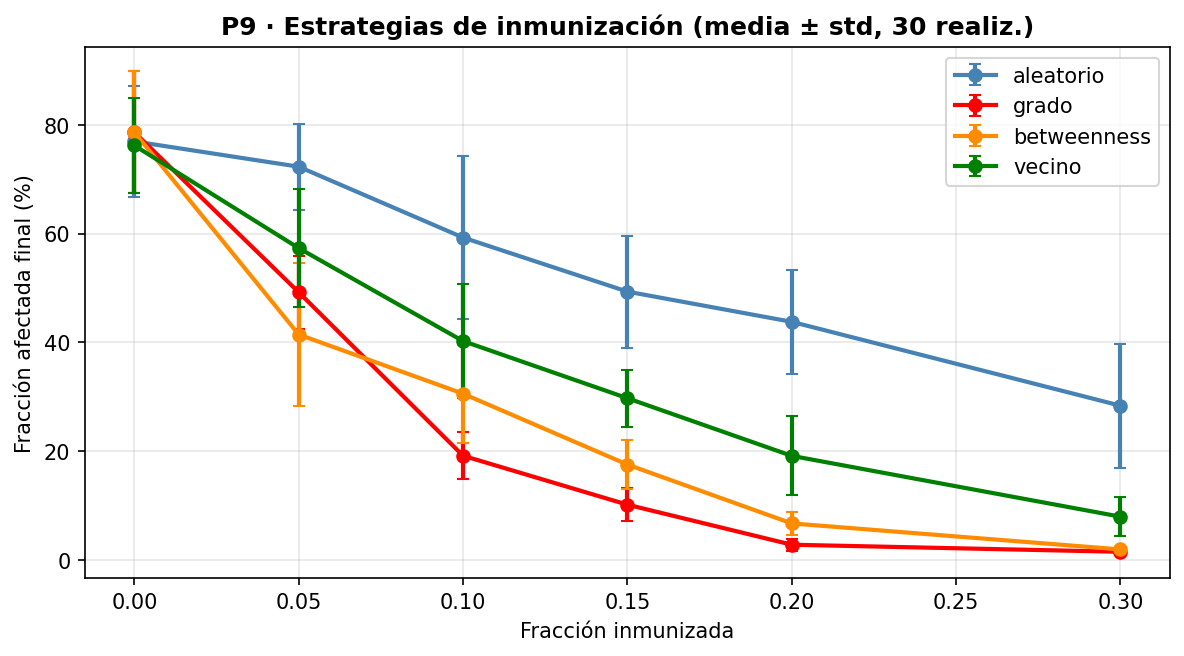
\includegraphics[width=0.75\linewidth]{images/p9_inmunizacion.png}
    \caption{Estrategias de inmunización: fracción afectada $R_{\text{final}}/n$
             vs.\ fracción inmunizada ($\beta = 0.372$, $\gamma = 0.1$).}
    \label{fig:inmunizacion}
\end{figure}

La Figura~\ref{fig:inmunizacion} compara cuatro estrategias de vacunación
(aleatoria, por grado, por betweenness y por vecino aleatorio) graficando
la fracción infectada final $R_{\infty}/n$ en función de la fracción de
nodos inmunizados.

Con solo el $20\%$ de nodos parcheados por grado (35 equipos), la fracción
infectada cae del $79\%$ al $4\%$. La estrategia por vecino logra resultados
similares sin conocer la topología completa, lo que la hace prácticamente
viable para el equipo de TI.

\subsection{Diagnóstico integrado: Índice de Criticidad Compuesto}

El P10 consolida los resultados de las fases 1--4 en un Índice de Criticidad
Compuesto:
\begin{equation}
    \text{ICC}_i = 0.35\,\hat{B}_i + 0.25\,A_i + 0.20\,C_i + 0.20\,\hat{D}_i
    \label{eq:icc}
\end{equation}

donde $\hat{B}_i$ es la betweenness normalizada, $A_i \in \{0,1\}$ indica
si el nodo es punto de articulación, $C_i \in \{0,1\}$ si pertenece al
corte mínimo, y $\hat{D}_i$ es el daño en cascada normalizado ($\alpha=0.1$).

\begin{figure}[H]
    \centering
    \begin{subfigure}[b]{0.56\linewidth}
        \centering
        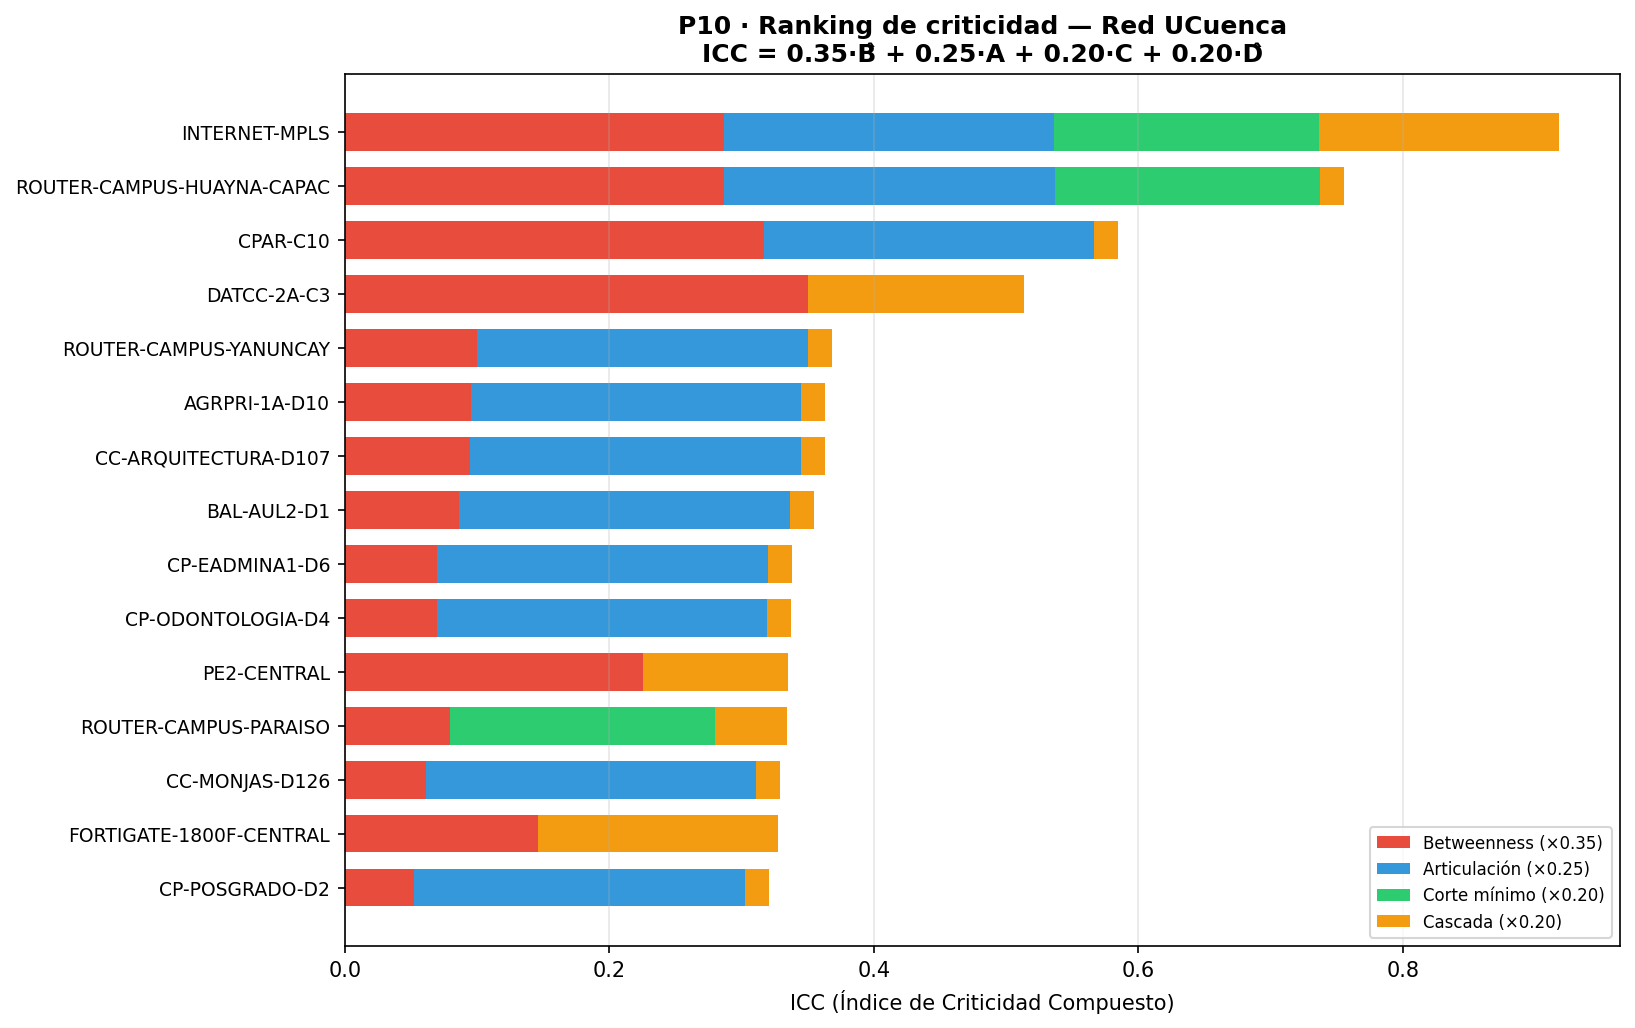
\includegraphics[width=\linewidth]{images/p10_ranking_icc.png}
        \caption{Ranking ICC — top 15 nodos (barras apiladas por componente).}
        \label{fig:ranking_icc}
    \end{subfigure}
    \hfill
    \begin{subfigure}[b]{0.40\linewidth}
        \centering
        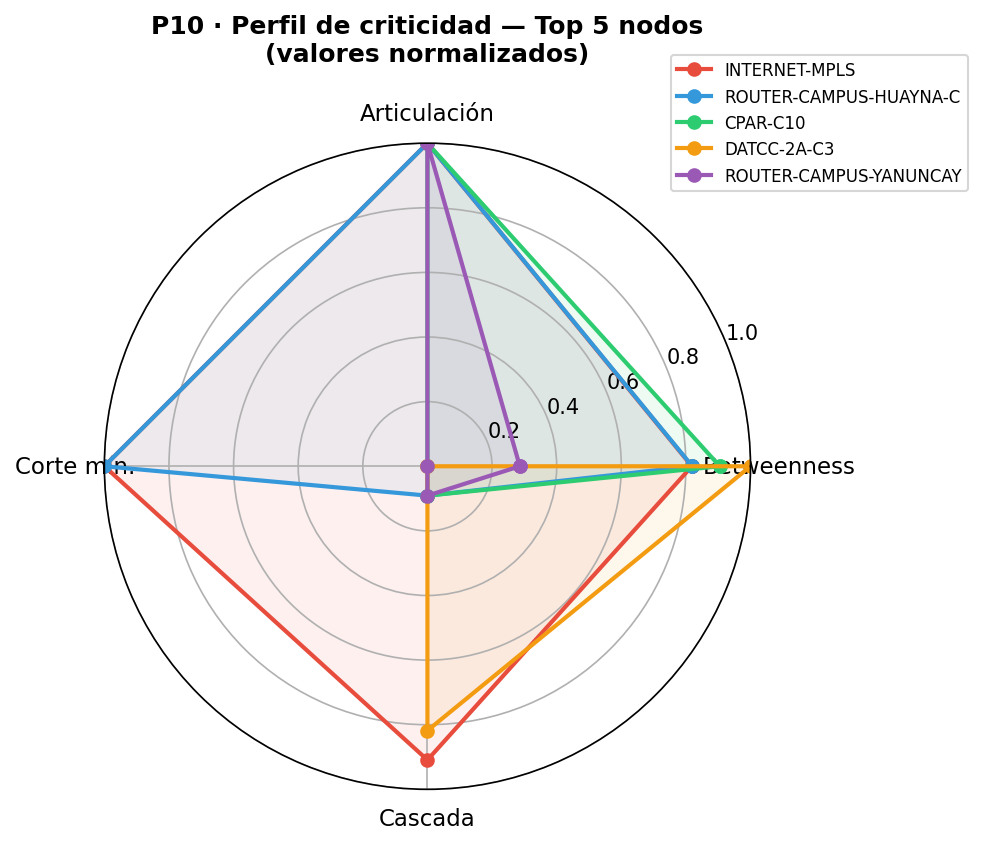
\includegraphics[width=\linewidth]{images/p10_radar_top5.png}
        \caption{Perfil de criticidad del top-5.}
        \label{fig:radar}
    \end{subfigure}
    \caption{Diagnóstico de puntos críticos mediante ICC.}
    \label{fig:icc}
\end{figure}

\begin{table}[H]
\centering
\caption{Top-10 nodos críticos (ICC) de la red UCuenca.}
\label{tab:top10}
\small
\begin{tabular}{C{0.6cm} L{4.2cm} L{2.8cm} C{1.2cm} C{1cm} C{1cm} C{1.2cm}}
    \toprule
    \encabezado{\#} &
    \encabezado{Nodo} &
    \encabezado{Campus} &
    \encabezado{ICC} &
    \encabezado{Art.} &
    \encabezado{Corte} &
    \encabezado{Capa} \\
    \midrule
    \rowcolor{tabfila}
    1 & INTERNET-MPLS              & MPLS         & 0.918 & \checkmark & \checkmark & MPLS \\
    2 & ROUTER-CAMPUS-HUAYNA-CAPAC & Paraíso      & 0.755 & \checkmark & \checkmark & WAN  \\
    \rowcolor{tabfila}
    3 & CPAR-C10                   & Paraíso      & 0.585 & \checkmark & ---        & Core \\
    4 & DATCC-2A-C3                & Central      & 0.514 & ---        & ---        & Core \\
    \rowcolor{tabfila}
    5 & ROUTER-CAMPUS-YANUNCAY     & Yanuncay     & 0.368 & \checkmark & ---        & WAN  \\
    6 & AGRPRI-1A-D10              & Yanuncay     & 0.363 & \checkmark & ---        & Agr. \\
    \rowcolor{tabfila}
    7 & CC-ARQUITECTURA-D107       & Central      & 0.363 & \checkmark & ---        & Agr. \\
    8 & BAL-AUL2-D1                & Balzay       & 0.355 & \checkmark & ---        & Agr. \\
    \rowcolor{tabfila}
    9 & CP-EADMINA1-D6             & Paraíso      & 0.338 & \checkmark & ---        & Agr. \\
    10& CP-ODONTOLOGIA-D4          & Paraíso      & 0.338 & \checkmark & ---        & Agr. \\
    \bottomrule
\end{tabular}
\end{table}

La Figura~\ref{fig:icc}a presenta el ranking de los 15 nodos más críticos
mediante barras apiladas que descomponen el ICC en sus cuatro componentes
($\hat{B}$, $A$, $C$, $\hat{D}$), permitiendo identificar qué factor
domina en cada nodo. La Figura~\ref{fig:icc}b muestra el perfil radar del
top-5, donde cada eje corresponde a una componente del ICC normalizada.
La Tabla~\ref{tab:top10} lista los 10 nodos de mayor ICC con sus valores
desagregados y la pertenencia a corte mínimo o punto de articulación.

Un resultado notable: \texttt{DATCC-2A-C3} (el más central por betweenness
y grado) ocupa el puesto~4 porque \textit{no} es punto de articulación
gracias a la redundancia con \texttt{DATCC-2A-C2}. En cambio,
\texttt{INTERNET-MPLS} ocupa el primer lugar porque cumple simultáneamente
las cuatro condiciones del ICC.

% ============================================================
%  8. PROPUESTA DE REDISEÑO — FASE 5
% ============================================================
\section{Propuesta de rediseño (Fase~5)}

\subsection{Los cinco enlaces propuestos}

Con base en el ranking ICC, se proponen cinco enlaces de redundancia sujetos
a la restricción dura de no superar cinco cambios de topología.
La Tabla~\ref{tab:enlaces} describe cada enlace propuesto, su capacidad y
el problema estructural específico que resuelve según el diagnóstico ICC.

\begin{table}[H]
\centering
\caption{Cinco enlaces propuestos y problema del diagnóstico que resuelve cada uno.}
\label{tab:enlaces}
\footnotesize
\begin{tabular}{C{0.4cm} L{4cm} C{1.6cm} L{6cm}}
    \toprule
    \encabezado{\#} &
    \encabezado{Enlace} &
    \encabezado{Cap. (Mbps)} &
    \encabezado{Problema que resuelve (ICC)} \\
    \midrule
    \rowcolor{tabfila}
    E1 & CPAR-C10 $\to$ INTERNET-MPLS             & 1\,000  & Elimina ROUTER-CAMPUS-HUAYNA-CAPAC (\#2) como punto único de paso hacia Internet \\
    E2 & DATCC-2A-C3 $\leftrightarrow$ CPAR-C10   & 10\,000 & Ruta directa 10~Gbps entre cores Central y Paraíso; reduce daño en cascada de \#3 y \#4 \\
    \rowcolor{tabfila}
    E3 & ROUTER-CAMPUS-YANUNCAY $\to$ PE2-CENTRAL & 1\,000  & Elimina ROUTER-CAMPUS-YANUNCAY (\#5) como articulación \\
    E4 & CP-ODONTOLOGIA-D4 $\leftrightarrow$ CP-EADMINA1-D6 & 1\,000 & Cross-link entre nodos de agregación (\#9 y \#10) en Campus Paraíso \\
    \rowcolor{tabfila}
    E5 & BAL-EADM-D3 $\to$ DT-0A-C13             & 1\,000  & Segundo uplink para switch de administración de Balzay \\
    \bottomrule
\end{tabular}
\end{table}

\subsection{Cuantificación: tabla antes / después / variación}

La Tabla~\ref{tab:antes_despues} cuantifica el impacto de los cinco
enlaces propuestos comparando las métricas clave de la red antes y después
de la intervención, junto con la variación absoluta y porcentual.

\begin{table}[H]
\centering
\caption{Métricas antes y después de la intervención (cinco enlaces ICC).}
\label{tab:antes_despues}
\small
\begin{tabular}{L{4.5cm} C{2.5cm} C{2.5cm} C{2cm} C{2cm}}
    \toprule
    \encabezado{Métrica} &
    \encabezado{Antes} &
    \encabezado{Después} &
    \encabezado{$\Delta$ abs.} &
    \encabezado{$\Delta$ \%} \\
    \midrule
    \rowcolor{tabfila}
    Aristas totales            & 209        & 214        & $+5$      & $+2.4$  \\
    Puentes                    & 141        & 137        & $-4$      & $-2.8$  \\
    \rowcolor{tabfila}
    Puntos de articulación     & 47         & 46         & $-1$      & $-2.1$  \\
    Distancia media (saltos)   & 5.830      & 4.976      & $-0.855$  & $\mathbf{-14.7}$ \\
    \rowcolor{tabfila}
    Eficiencia global $E_0$    & 0.2082     & 0.2330     & $+0.025$  & $\mathbf{+11.9}$ \\
    $\fc$ ataque por grado     & 0.011      & 0.011      & 0         & 0       \\
    \rowcolor{tabfila}
    Flujo Campus Central       & 5\,000 Mb  & 6\,318 Mb  & $+1\,318$ & $+26.4$ \\
    Flujo Campus Paraíso       & 318 Mb     & 6\,318 Mb  & $+6\,000$ & $\mathbf{\times 19}$ \\
    \rowcolor{tabfila}
    Flujo Campus Balzay        & 3\,290 Mb  & 3\,290 Mb  & 0         & 0       \\
    Flujo Campus Yanuncay      & 1\,000 Mb  & 1\,000 Mb  & 0         & 0       \\
    \bottomrule
\end{tabular}
\end{table}

La Figura~\ref{fig:percolacion_p11} evalúa la robustez de la propuesta bajo
ataque dirigido: el panel izquierdo muestra la eficiencia global $E(f)$
a medida que se eliminan nodos por betweenness, y el panel derecho la
distancia media dentro de la componente gigante. La red rediseñada mantiene
mayor eficiencia y menor distancia que la original para toda $f$, confirmando
la mejora estructural.

\begin{figure}[H]
    \centering
    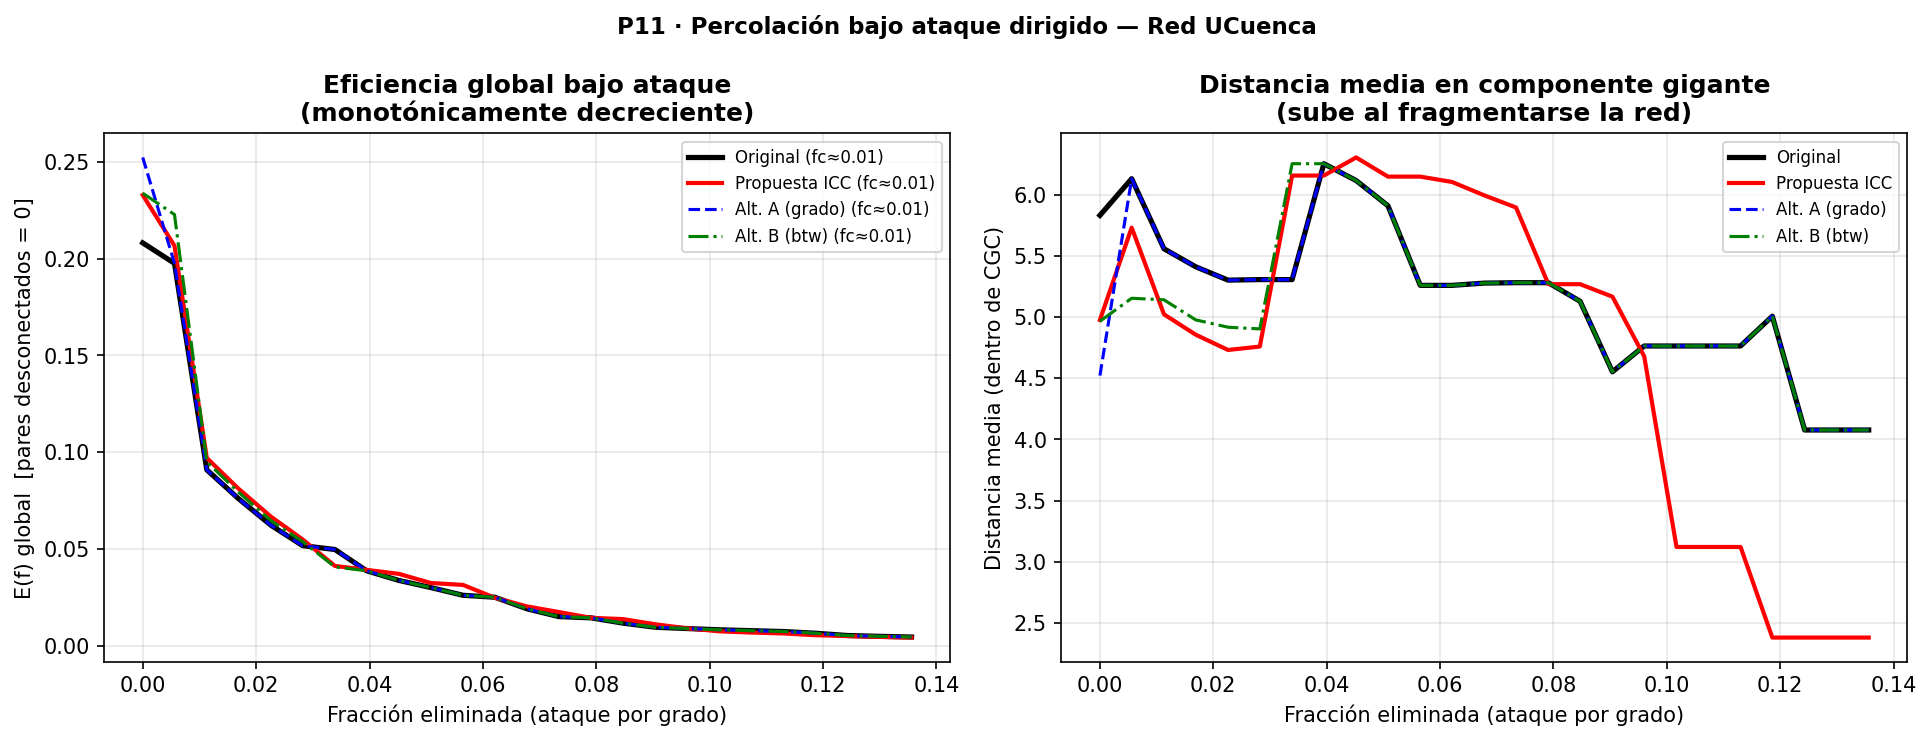
\includegraphics[width=\linewidth]{images/p11_percolacion_comparacion.png}
    \caption{Percolación bajo ataque dirigido. \textbf{Izquierda:} eficiencia
             global sobre todos los pares originales (pares desconectados~$= 0$,
             curva monotónicamente decreciente). \textbf{Derecha:} distancia
             media dentro de la componente gigante restante.}
    \label{fig:percolacion_p11}
\end{figure}

La Figura~\ref{fig:flujo_p11} compara el flujo máximo por campus entre la
red original, la propuesta ICC y las dos alternativas evaluadas. Se observa
que solo la propuesta ICC resuelve el cuello de botella de Campus Paraíso
($\times 19$ en flujo disponible), gracias a que los enlaces propuestos
abordan directamente los nodos más críticos del ICC.

\begin{figure}[H]
    \centering
    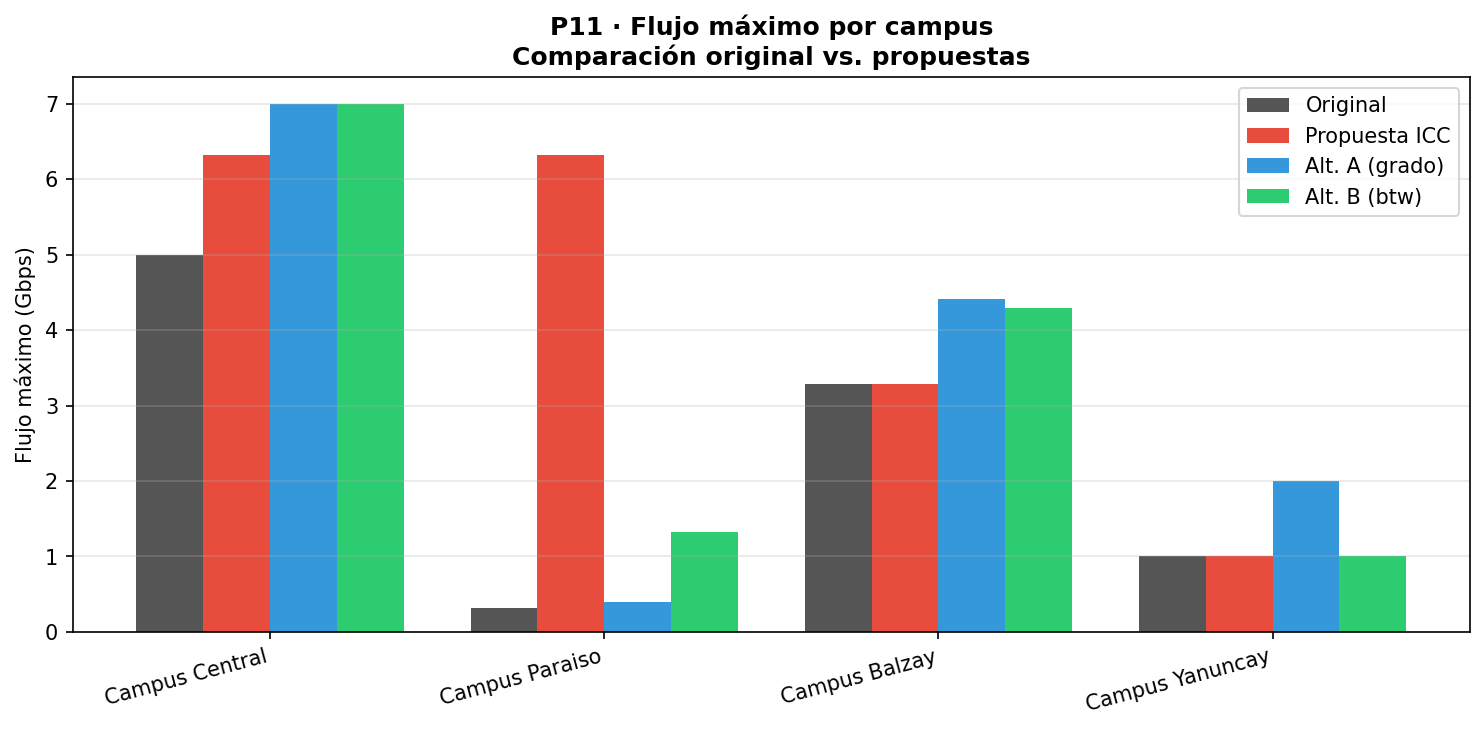
\includegraphics[width=0.75\linewidth]{images/p11_flujo_comparacion.png}
    \caption{Flujo máximo por campus: original vs.\ propuesta ICC vs.\
             alternativas.}
    \label{fig:flujo_p11}
\end{figure}

\subsection{Comparación contra alternativas}

La Tabla~\ref{tab:alternativas} compara la propuesta ICC con dos alternativas
de cinco enlaces: Alt.~A (conecta los pares de nodos de mayor grado) y
Alt.~B (conecta los nodos de mayor betweenness entre sí), evaluando el
impacto en puentes, articulaciones, distancia media, eficiencia global y
flujo por campus.

\begin{table}[H]
\centering
\caption{Propuesta ICC vs.\ dos alternativas de cinco enlaces.
         Alt.~A: conecta los pares de nodos de mayor grado.
         Alt.~B: conecta los nodos de mayor betweenness entre sí.}
\label{tab:alternativas}
\small
\begin{tabular}{L{4cm} C{2.2cm} C{2.2cm} C{2.2cm} C{2.2cm}}
    \toprule
    \encabezado{Métrica} &
    \encabezado{Original} &
    \encabezado{ICC (prop.)} &
    \encabezado{Alt.~A (grado)} &
    \encabezado{Alt.~B (btw)} \\
    \midrule
    \rowcolor{tabfila}
    Puentes          & 141    & 137    & 138    & 140   \\
    Articulaciones   & 47     & 46     & 45     & 46    \\
    \rowcolor{tabfila}
    Dist. media      & 5.830  & 4.976  & 4.521  & 4.966 \\
    Efic. global     & 0.2082 & 0.2330 & 0.2524 & 0.2339 \\
    \rowcolor{tabfila}
    Flujo Campus Paraíso & 318 Mb & \textbf{6\,318 Mb} & 395 Mb & 1\,318 Mb \\
    \bottomrule
\end{tabular}
\end{table}

La Alternativa~A mejora la eficiencia global ($+21.2\%$) y la distancia media
($-22.4\%$) más que la propuesta ICC, pero \textbf{no resuelve el problema más
crítico}: el flujo a Campus Paraíso sigue en solo 395~Mbps porque concentra
todos sus enlaces en \texttt{DATCC-2A-C3} sin abordar el cuello de botella
del router de campus. La Alternativa~B obtiene resultados similares a la
propuesta ICC en eficiencia, pero tampoco resuelve Campus Paraíso
(1\,318~Mbps vs.\ 6\,318~Mbps).

\begin{hallazgo}
\textbf{Justificación de la propuesta ICC:} es la única que dirige
simultáneamente los tres nodos del top-4 del ranking (\#2, \#3, \#4) y
produce la mejora operativamente más relevante: el flujo a Campus Paraíso
se multiplica por~19.
\end{hallazgo}

\subsection{Estimación de costo y factibilidad}

La factibilidad varía significativamente entre enlaces. E4 y E5 son
inmediatamente ejecutables con recursos internos de TI (cableado dentro de
un campus, $< 200$~m). E1 y E3 requieren contratar un segundo circuito MPLS
al proveedor, lo que implica un costo operativo mensual recurrente pero no
obra civil nueva si ya existe ducto al POP del ISP.

E2 (DATCC-2A-C3 $\leftrightarrow$ CPAR-C10) es el enlace de mayor impacto
y mayor costo: los campus Central y Paraíso están separados por varios
kilómetros urbanos. Requeriría fibra oscura o un circuito dedicado
inter-campus, con alta inversión inicial. Una alternativa transitoria sería
un túnel MPLS lógico sobre la infraestructura WAN existente, que no da
10~Gbps pero permite validar la topología antes del tendido físico.

% ============================================================
%  9. CONCLUSIONES Y LIMITACIONES
% ============================================================
\section{Conclusiones y limitaciones}

\subsection{Conclusiones}

\begin{enumerate}
    \item \textbf{La red UCuenca es jerárquica por diseño, no emergente, con
    heterogeneidad de grado significativa.} La densidad muy baja (0.013),
    el clustering casi nulo (0.034) y la asortatividad negativa ($r=-0.147$)
    son la firma estructural de la topología estrella core\,$\to$\,agregación\,$\to$\,acceso.
    El ajuste de ley de potencia ($\alpha=2.41$, $x_{\min}=3$) no puede
    confirmarse con rigor estadístico dado el tamaño reducido de la cola (20
    de 177 nodos, \textit{p}-value bootstrap~$=~0.754$), pero la heterogeneidad
    de grado produce la paradoja clásica: brecha de 7.5:1 entre robustez ante
    fallos aleatorios ($\fc = 0.75$) y ante ataques dirigidos ($\fc = 0.10$).

    \item \textbf{El nodo más crítico es INTERNET-MPLS, no DATCC-2A-C3.}
    El Índice de Criticidad Compuesto revela que el nodo con mayor betweenness
    (DATCC-2A-C3) no es el más peligroso porque tiene redundancia con
    DATCC-2A-C2. INTERNET-MPLS, que es simultáneamente punto de articulación,
    nodo del corte mínimo y generador de cascadas, tiene ICC~$= 0.918$ y su
    falla impacta a toda la institución.

    \item \textbf{Campus Paraíso es el punto de mayor vulnerabilidad de flujo.}
    Con solo 318~Mbps de flujo máximo disponible (frente a 43\,000~Mbps del
    Campus Central), cualquier incidente en ROUTER-CAMPUS-HUAYNA-CAPAC aísla
    completamente al campus. La intervención E1+E2 resuelve este problema
    con un impacto de $\times$19 en flujo disponible.

    \item \textbf{Las comunidades Louvain coinciden con la geografía.}
    La modularidad $Q = 0.73$ confirma que la red fue diseñada con
    separación clara por campus. Este diseño facilita la contención de fallos
    pero implica que los routers de campus son puntos únicos de falla para
    toda su comunidad.

    \item \textbf{Cinco enlaces bien elegidos mejoran la operación pero no
    cambian el perfil de vulnerabilidad ante ataques.} La propuesta ICC
    eleva la eficiencia global en 11.9\% y multiplica por 19 el flujo hacia
    Campus Paraíso. Sin embargo, $\fc$ bajo ataque dirigido no varía (0.011
    antes y después): mejorar la operación normal y blindar contra ataques
    deliberados son objetivos distintos que requieren intervenciones distintas.
    La redundancia real ante ataques requeriría duplicar el core, no solo
    añadir enlaces en la periferia.
\end{enumerate}

\subsection{Limitaciones}

El análisis presenta las siguientes limitaciones que deben considerarse al
interpretar los resultados:

\begin{itemize}
    \item \textbf{Datos estáticos.} El grafo se construyó a partir de
    diagramas de red, no de mediciones en tiempo real. Los valores de
    capacidad (Mbps) son nominales, no tráfico real cursado. Un análisis
    operativo requeriría datos de NetFlow o SNMP en producción.

    \item \textbf{Modelo de carga simplificado.} El betweenness como proxy
    de carga supone enrutamiento por caminos más cortos, pero la red usa
    OSPF con métricas configuradas que pueden diferir significativamente de
    la ruta topológicamente más corta.

    \item \textbf{Cascadas sin mecanismos de protección.} El modelo
    Motter-Lai no contempla Spanning Tree, HSRP/VRRP ni Fast Reroute MPLS,
    que en la práctica limitan las cascadas. Los resultados sobrestiman el
    daño en cascada.

    \item \textbf{Optimización de los cinco enlaces no es exacta.} Encontrar
    el conjunto óptimo de $k$ enlaces es un problema NP-difícil. La propuesta
    ICC usa heurística guiada por el ranking, que puede no ser globalmente
    óptima. Análogamente, la heurística voraz para \textit{p}-Centro (P7)
    produce un gap de hasta 100\% frente al óptimo exacto: ninguna heurística
    estructural debe asumirse globalmente óptima sin verificación.

    \item \textbf{Topología lógica, no física.} No se modelaron túneles VPN,
    VLANs ni rutas OSPF alternativas que existen a nivel lógico y podrían
    cambiar el análisis de robustez real.
\end{itemize}

% ============================================================
%  10. REFERENCIAS
% ============================================================
\section*{Referencias}
\begin{thebibliography}{99}

\bibitem{barabasi1999}
Barabási, A.-L., \& Albert, R. (1999).
Emergence of scaling in random networks.
\textit{Science}, \textit{286}(5439), 509--512.
\url{https://doi.org/10.1126/science.286.5439.509}

\bibitem{watts1998}
Watts, D. J., \& Strogatz, S. H. (1998).
Collective dynamics of `small-world' networks.
\textit{Nature}, \textit{393}(6684), 440--442.
\url{https://doi.org/10.1038/30918}

\bibitem{newman2010}
Newman, M. E. J. (2010).
\textit{Networks: An Introduction}.
Oxford University Press.

\bibitem{motter2002}
Motter, A. E., \& Lai, Y.-C. (2002).
Cascade-based attacks on complex networks.
\textit{Physical Review E}, \textit{66}(6), 065102.
\url{https://doi.org/10.1103/PhysRevE.66.065102}

\bibitem{pastor2001}
Pastor-Satorras, R., \& Vespignani, A. (2001).
Epidemic spreading in scale-free networks.
\textit{Physical Review Letters}, \textit{86}(14), 3200--3203.
\url{https://doi.org/10.1103/PhysRevLett.86.3200}

\bibitem{blondel2008}
Blondel, V. D., Guillaume, J.-L., Lambiotte, R., \& Lefebvre, E. (2008).
Fast unfolding of communities in large networks.
\textit{Journal of Statistical Mechanics: Theory and Experiment},
\textit{2008}(10), P10008.
\url{https://doi.org/10.1088/1742-5468/2008/10/P10008}

\bibitem{clauset2009}
Clauset, A., Shalizi, C. R., \& Newman, M. E. J. (2009).
Power-law distributions in empirical data.
\textit{SIAM Review}, \textit{51}(4), 661--703.
\url{https://doi.org/10.1137/070710111}

\bibitem{albert2000}
Albert, R., Jeong, H., \& Barabási, A.-L. (2000).
Error and attack tolerance of complex networks.
\textit{Nature}, \textit{406}(6794), 378--382.
\url{https://doi.org/10.1038/35019019}

\bibitem{erdos1959}
Erdős, P., \& Rényi, A. (1959).
On random graphs I.
\textit{Publicationes Mathematicae Debrecen}, \textit{6}, 290--297.

\bibitem{astudillo2026}
Astudillo-Salinas, F. (2026).
\textit{Módulo 1217 --- Redes Complejas: material del curso}.
Universidad de Cuenca.
\url{https://github.com/fabianastudillo/ComplexNetworks}

\bibitem{networkx}
Hagberg, A. A., Schult, D. A., \& Swart, P. J. (2008).
Exploring network structure, dynamics, and function using NetworkX.
En G.~Varoquaux, T.~Vaught, \& J.~Millman (Eds.),
\textit{Proceedings of the 7th Python in Science Conference} (pp.~11--15).

\end{thebibliography}

% ============================================================
%  11. ANEXOS
% ============================================================
\section*{Anexos}

\subsection*{A. Resultados numéricos extendidos}

Los archivos CSV con todos los resultados numéricos están disponibles en la
carpeta \code{results/tablas/}. Los archivos más relevantes son:

\begin{itemize}
    \item \code{p1\_centralidades\_top10.csv} --- top-10 por cuatro métricas
    \item \code{p6\_flujo\_por\_campus.csv} --- flujo máximo por campus
    \item \code{p8\_percolacion\_nodos.csv} --- curvas de robustez (100
          realizaciones)
    \item \code{p9\_cascada\_tolerancia.csv} --- cascada vs.\ tolerancia
          $\alpha$
    \item \code{p10\_icc\_todos.csv} --- ICC de los 177 nodos
    \item \code{p11\_metricas\_comparacion.csv} --- tabla antes/después para
          las cuatro variantes
\end{itemize}

\subsection*{B. Código fuente}

El código está organizado en once scripts Python en \code{src/}:

\begin{center}
\small
\begin{tabular}{ll}
    \toprule
    \textbf{Archivo} & \textbf{Contenido} \\
    \midrule
    \code{problema1.py}  & Métricas básicas, centralidades, ley de potencia \\
    \code{problema2.py}  & Modelos nulos, visualización de la red \\
    \code{problema3.py}  & BFS, DFS, k-core, ciclos \\
    \code{problema4.py}  & Comunidades Louvain y k-means \\
    \code{problema5.py}  & Dijkstra y Floyd-Warshall \\
    \code{problema6.py}  & Flujo máximo, corte mínimo, flujo de costo mínimo \\
    \code{problema7.py}  & p-Mediana y p-Centro \\
    \code{problema8.py}  & Percolación de nodos y aristas \\
    \code{problema9.py}  & Cascadas Motter-Lai y modelo SIR \\
    \code{problema10.py} & Índice de Criticidad Compuesto \\
    \code{problema11.py} & Propuesta de rediseño y comparación \\
    \bottomrule
\end{tabular}
\end{center}

Repositorio: \url{https://github.com/} \textit{(completar enlace)}

\subsection*{C. Verificación del grafo}

El pipeline de carga (\code{cargar\_red.py}) verifica automáticamente 13
invariantes del grafo en cada ejecución:

\begin{itemize}
    \item $n = 177$, $m = 209$, 1 componente conexa
    \item Nodos por capa: acceso~132, agregación~27, core~5
    \item Aristas por rol: principal~157, WAN~32, respaldo~12,
          secundario~5, inferido~3
    \item Aristas con campo \code{trafico\_mbps}: 170
    \item Aristas con campo \code{capacidad\_mbps}: 28
\end{itemize}

Todas las verificaciones pasan en la versión actual del grafo.

\end{document}
